\chapter{模的演算}\label{ch:calculus-of-modules}


∞-范畴之间的\trModule{}的演算，与\trUnitalRing{}之间的（双）模的演算极为相似。这里，
∞-范畴顶替了环的位置，∞-范畴之间的\trFunctor{}扮演环同态的角色；在下表中，我们
把\trFunctor{}竖直展示。从 $A$ 到 $B$ 的\trModule{} $E$，一如第 7 章所考虑的那
些\trTwoSidedFibration，是一个∞-范畴：$A$「作用于左侧」，$B$「作用于右侧」，而
这两种作用相互交换；这与环论中 $A$–$B$ 双模的记法相类似，也解释了我们选用这一
术语的缘由。今后每当无须为其构成\trSpan{}的两条腿显式命名时，%
\trModule{} $A\xleftarrow{q}E\xrightarrow{p}B$ 就将被描绘为 $A\xrightarrow{E}B$。

\begin{center}
\begin{tabular}{c@{\hspace{5em}}c@{\hspace{5em}}c}
\trUnitalRing & $A$ & \trInfinityCategories\\[14pt]
环同态 &
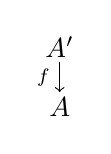
\begin{tikzpicture}[baseline={(current bounding box.center)},x=1.5em,y=1.2em]
  \node (Ap) at (0,0.9)  {$A'$};
  \node (A)  at (0,-0.9) {$A$};
  \draw[->] (0,0.45) -- node[left]{$\scriptstyle f$} (0,-0.45);
\end{tikzpicture} & \trInfinityFunctor\\[14pt]
环之间的双模 & $A\xrightarrow{E}B$ & ∞-范畴之间的\trModule\\[14pt]
模映射 &
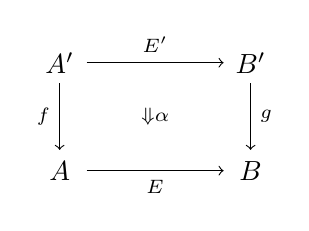
\begin{tikzpicture}[baseline={(current bounding box.center)},x=1.5em,y=1.5em]
  \node (Ap) at (0,1.3)    {$A'$};
  \node (Bp) at (4.6,1.3)  {$B'$};
  \node (A)  at (0,-1.3)   {$A$};
  \node (B)  at (4.6,-1.3) {$B$};
  \draw[->] (0.65,1.3) -- node[above]{$\scriptstyle E'$} (3.95,1.3);
  \draw[->] (0.65,-1.3) -- node[below]{$\scriptstyle E$} (3.95,-1.3);
  \draw[->] (0,0.8) -- node[left]{$\scriptstyle f$} (0,-0.8);
  \draw[->] (4.6,0.8) -- node[right]{$\scriptstyle g$} (4.6,-0.8);
  \node at (2.3,0) {$\scriptstyle\Downarrow\alpha$};
\end{tikzpicture} & 模映射
\end{tabular}
\end{center}

最后，还有一种模映射的概念，其边界是如上所示的一个由两个\trModule{}与两个%
\trFunctor{}组成的方块。在环论中，具有这种边界的模映射由一支 $A'$–$B'$ 模同态
$E'\to E(g,f)$ 给出，余定义域则是一个 $A'$–$B'$ 双模，由把 $A$–$B$ 模 $E$ 中的
标量乘法沿环同态 $f$ 与 $g$ 作限制而定义。一个类似的想法已由定义 8.1.4 编码。

这一类比还要延伸得更深：\trUnitalRing、环同态、双模与模映射定义了一个 Wood $[132]$
意义下的\emph{\trProarrowEquipment}（proarrow equipment）。\footnote{这可以视为下面这个
原型装备的一个特例：对任何封闭对称幺半范畴 $\mathcal{V}$，由 $\mathcal{V}$-范畴、
$\mathcal{V}$-函子、$\mathcal{V}$-模以及它们之间的 $\mathcal{V}$-%
\trNaturalTransformation{}构成的装备。环的装备则由「取 $\mathcal{V}$ 为%
\trAbelianGroup{}\trCategory」这一情形，再限制到具单一对象的%
\trAbelianGroup{}\trEnrichedCategory{}之上而得到。}
我们在本章中的主要结果是定理 8.2.6，它断言：任一\trInfinityCosmos{}中的
∞-范畴、\trFunctor、\trModule{}与模映射定义一个 Cruttwell 与 Shulman $[32]$
意义下的\emph{\trVirtualEquipment}（virtual equipment）。

作为第一步，我们将在 8.1 节中引入双侧等价纤维化的\trDoubleCategory，它经限制
而定义一个模的\emph{\trVirtualDoubleCategory}（virtual double category）。
\emph{\trDoubleCategory}（double category）是一种 2 维的范畴：它拥有对象；拥有
两种\trOneMorphism{}，即「水平的」与「竖直的」；还拥有装入「方块」之中的 2 维\trCell，
这些方块的边界由定义域与余定义域相容的水平与竖直\trOneMorphism{}构成（见定义 B.1.9）。
抽象代数中一个富有启发性的例子是模的\trDoubleCategory：对象为环，竖直态射为
环同态，水平态射为双模，而方块为双模同态。竖直复合就是复合同态，这是一个严格
结合且幺的运算；水平复合则由\trModule{}的\trTensorProduct{}给出，后者在相干自然同构
的意义下结合且幺。在文献中，这类结构有时被称作\emph{\trPseudoDoubleCategory}（pseudo double category）——态射与方块在「竖直」方向上严格复合，而在「水平」方向上仅到同构为
止——不过，由于它是正文中考虑的唯一类型，我们径称之为「\trDoubleCategory」。
\footnote{严格\trDoubleCategory{}在定理 B.3.6 中短暂露面，用以表达对应
（mates correspondence）的函子性。}

我们在 8.1 节中的目标，是描述一个类似的结构：其对象与竖直态射是任一取定的%
\trInfinityCosmos{}中的\trInfinityCategories{}与\trFunctor，其水平态射是%
\trModule，其方块是模映射。若把水平态射换成更大的一类——\trTwoSidedFibration
——或还要更大的一类——\trTwoSidedIsofibration——则这些态射便组装成一个%
\trDoubleCategory，其水平复合运算由命题 7.2.6 定义（见命题 8.1.6）。
然而，这一水平复合运算并不保持\trModule：\trArrowInfinityCategory{} $A^{2}$ 定义一个从 $A$ 到
$A$ 的\trModule，它与自身的水平复合\trEquivalence{}于命题 7.1.6 的那条双侧纤维
化 $(p_{2},p_{0})\colon A^{3}\twoheadrightarrow A\times A$，而后者在
$A\times A$ 之上的\trSliceInfinityCosmos{}中不是\trDiscrete。要定义一个真正的
「模的\trTensorProduct{}」运算，需要一个两阶段的构造：先如命题 7.2.6 那样作出定义复
合双侧纤维化的那个\trPullback，再经某种「\trHomotopyCoinverter{}」（homotopy coinverter）
构造，把所得者反射成一条\emph{\trDiscrete{}}双侧\trFibration。由于所涉的余极限
不在\trInfinityCosmos{}诸公理的辖域之内，这就多少构成了一个障碍。\footnote{%
实践中遭遇到的\trInfinityCosmos{}事实上容许一切柔性的加权\trHomotopy\trColimit
——特别是包括\trHomotopyCoinverter{}——因为它们按 Bourke、Lack 与 Vokřínek $[22]$ 所定义
的一种意义，往往是\emph{\trAccessible}（accessible）（见题外话 E.1.8）。}

我们并不打算为了追求一个模的\trDoubleCategory{}而踏出公理框架的舒适区，转而描
述在这一公理化体系之内自然出现的结构——事后证明，范畴论学家对它颇为熟悉，而
它也足够稳健，足以胜任我们想要的应用。我们首先证明：∞-范畴、\trFunctor、%
\trModule{}与模映射组装成一个\emph{\trVirtualDoubleCategory}——一种比%
\trDoubleCategory{}更弱的结构，其中容许\trCell{}具有多元的水平源，以此作为模的
水平复合的一种「虚拟」替代。\trVirtualDoubleCategory{}之于\trDoubleCategory，
恰如多范畴之于\trMonoidalCategory{}；事实上，\trVirtualDoubleCategory{}正是相对于有向图上
的\trFreeCategory{}单子而定义的那些「广义多范畴」$[32, 76]$。

\emph{\trVirtualEquipment}是一个满足两条附加公理的\trVirtualDoubleCategory。
其中一条提供一种「\trRestrictionOfScalars{}」运算，使得水平态射 $A\xrightarrow{E}B$ 得以沿一
对竖直态射 $f\colon A'\to A$ 与 $g\colon B'\to B$ 被\trPullback；另一条要求每
个对象都拥有一支水平的「单位」态射，它满足某个适当的\trUniversalProperty，在
缺乏复合运算之时充当幺性复合规则的替代。一旦 8.2 节给出了%
\trVirtualEquipment{}的定义，这两条公理便可由第 7 章的诸结果轻易推出。最后两
节致力于探索这一结构的诸推论；在第 9 章发展∞-范畴的形式范畴论时，这些推论将
得到充分的运用。在 8.3 节中，我们将说明如何在\trVirtualEquipment{}中识别模的
某些水平复合，即使任意一对可复合的\trModule{}的\trTensorProduct{}的一般构造尚属未
知。最后的 8.4 节汇集了由∞-范畴之间的\trFunctor{} $k\colon A\to B$ 所表示的
诸\trModule{}
$A\xrightarrow{\mathrm{Hom}_{B}(B,k)}B$ 与
$B\xrightarrow{\mathrm{Hom}_{B}(k,B)}A$ 的许多特殊性质，并重温 3.5 节中首次建
立的某些性质。

\providecommand{\Mod}{\mathbb{M}od}
\providecommand{\Fun}{\operatorname{Fun}}
\providecommand{\rvnullpair}{\vcenter{\hbox{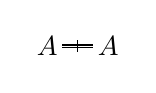
\begin{tikzpicture}[x=1em,y=1em]%
\node (rva) at (0,0) {$A$};\node (rvb) at (2.2,0) {$A$};%
\draw[double] (0.55,0) -- (1.65,0);\draw (1.1,0.22) -- (1.1,-0.22);\end{tikzpicture}}}}

\section{双侧等价纤维化的\trDoubleCategory}\label{sec:double-category-of-two-sided-isofibrations}

回忆推论 7.4.4：\trModule{}的\trInfinityCosmos{}既可定义为%
\trTwoSidedFibration{}的\trInfinityCosmos{}的一个全子范畴，也可定义为%
\trTwoSidedIsofibration{}的\trInfinityCosmos{}的一个全子范畴。
这为构造模的\trVirtualDoubleCategory{}摆出了两条路线：它既可以实现为双侧纤维化的\trDoubleCategory{}的
一个全子范畴，也可以实现为双侧等价纤维化的\trDoubleCategory{}的一个全子范畴。我们采纳
后者，因为它略为简单；不过也邀请读者改走前一条路线（见%
\cref{ex:map-of-two-sided-fibrations}）。

我们的第一项任务，是定义将要引入的那些\trDoubleCategory{}中的 2 维态射。

\begin{definition}\label{def:fibered-map-of-two-sided-isofibrations}
从 $A\overset{q}{\twoheadleftarrow}E\overset{p}{\twoheadrightarrow}B$ 到
$A\overset{s}{\twoheadleftarrow}F\overset{r}{\twoheadrightarrow}B$ 的一支%
\textbf{双侧等价纤维化间的纤维化映射}（fibered map of two-sided
isofibrations），是一个由严格交换的\trFunctor{}构成的纤维化同构类
\begin{center}
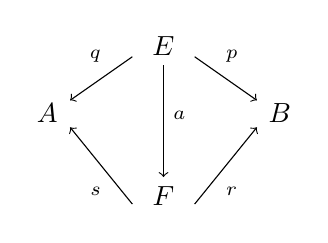
\begin{tikzpicture}[x=1.5em,y=1.5em]
  \node (E) at (0,1.6)  {$E$};
  \node (A) at (-2.8,0) {$A$};
  \node (B) at (2.8,0)  {$B$};
  \node (F) at (0,-2.0) {$F$};
  \draw[->] (-0.75,1.35) -- node[above left,pos=0.35]{$\scriptstyle q$} (-2.25,0.3);
  \draw[->] (0.75,1.35)  -- node[above right,pos=0.35]{$\scriptstyle p$} (2.25,0.3);
  \draw[->] (0,1.15) -- node[right,pos=0.45]{$\scriptstyle a$} (0,-1.55);
  \draw[->] (-0.75,-2.2) -- node[below left,pos=0.35]{$\scriptstyle s$} (-2.25,-0.35);
  \draw[->] (0.75,-2.2)  -- node[below right,pos=0.35]{$\scriptstyle r$} (2.25,-0.35);
\end{tikzpicture}
\end{center}
其中两支这样的\trFunctor{} $a$ 与 $a'$ 被视为等价的，当存在自然同构
$\gamma\colon a\cong a'$ 使得 $s\gamma=\mathrm{id}_{q}$ 且
$r\gamma=\mathrm{id}_{p}$。

当 $A\overset{q}{\twoheadleftarrow}E\overset{p}{\twoheadrightarrow}B$ 与
$A\overset{s}{\twoheadleftarrow}F\overset{r}{\twoheadrightarrow}B$ 是%
\trModule{}时，我们把二者之间的纤维化映射称作从 $E$ 到 $F$ 的%
\textbf{模的纤维化映射}（fibered map of modules）。
\end{definition}

\begin{observation}[模与纤维化映射的 1-范畴]\label{obs:one-categories-of-modules}
∞-宇宙 $\mathcal{K}$ 中从 $A$ 到 $B$ 的双侧等价纤维化连同纤维化映射一起
构成的 1-范畴可以这样得到：取以\trQuasiCategory{}富集的范畴
$\mathcal{K}_{/A\times B}$ 的一个商，或取其\trHomotopyTwoCategory{}
$\mathfrak{h}(\mathcal{K}_{/A\times B})$ 的一个商，或取切片%
\trHomotopyTwoCategory{} $\mathfrak{h}\mathcal{K}_{/A\times B}$ 的一个商。
这个商 1-范畴拥有同一批对象，并以诸\trFunctor{}的\trIsomorphism{}类作为
其态射。

由引理 7.4.3，从 $A$ 到 $B$ 的\trModule{}连同纤维化映射一起构成的 1-范畴
是一个全子范畴；或者换个说法，可以同法把它视为以\trKanComplex{}富集的
范畴 ${}_{A\backslash}\Mod(\mathcal{K})_{/B}$ 的商，或其%
\trHomotopyTwoCategory{} $\mathfrak{h}({}_{A\backslash}\Mod(\mathcal{K})_{/B})$
的商。
\end{observation}

\cref{obs:one-categories-of-modules}的诸 1-范畴之所以有趣，是因为它们恰好
捕捉了定义 3.2.7 中首次引入的、双侧等价纤维化之间或模之间的那个正确的%
\trEquivalence{}概念。

\begin{lemma}\label{lem:one-category-equivalences}
在∞-宇宙 $\mathcal{K}$ 中：
\begin{enumerate}[label=(\roman*)]
\item 一对双侧等价纤维化在 $\mathcal{K}_{/A\times B}$ 中\trEquivalence{}，
当且仅当它们在从 $A$ 到 $B$ 的双侧等价纤维化的 1-范畴中\trIsomorphism{}；
\item 一对\trModule{}在 $A\times B$ 之上\trEquivalence{}，当且仅当它们在从
$A$ 到 $B$ 的模的 1-范畴中\trIsomorphism{}。
\end{enumerate}
\end{lemma}

刚才呈现的每一个定义都容有一个共同的推广，它定义了居于方块之中的那些
2 维映射。

\begin{definition}[方块中的映射]\label{def:maps-in-squares}
从 $A'\overset{q'}{\twoheadleftarrow}E'\overset{p'}{\twoheadrightarrow}B'$
到 $A\overset{q}{\twoheadleftarrow}E\overset{p}{\twoheadrightarrow}B$ 的、
位于 $f\colon A'\to A$ 与 $g\colon B'\to B$ 之上的一个\textbf{模映射}
（map of modules）或\textbf{双侧等价纤维化映射}（map of two-sided
isofibrations）描绘如下
\begin{center}
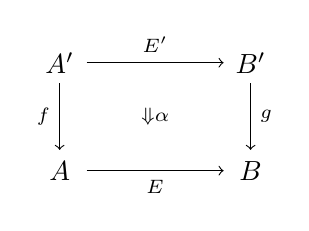
\begin{tikzpicture}[x=1.5em,y=1.5em]
  \node (Ap) at (0,1.3)    {$A'$};
  \node (Bp) at (4.6,1.3)  {$B'$};
  \node (A)  at (0,-1.3)   {$A$};
  \node (B)  at (4.6,-1.3) {$B$};
  \draw[->] (0.65,1.3) -- node[above]{$\scriptstyle E'$} (3.95,1.3);
  \draw[->] (0.65,-1.3) -- node[below]{$\scriptstyle E$} (3.95,-1.3);
  \draw[->] (0,0.8) -- node[left]{$\scriptstyle f$} (0,-0.8);
  \draw[->] (4.6,0.8) -- node[right]{$\scriptstyle g$} (4.6,-0.8);
  \node at (2.3,0) {$\scriptstyle\Downarrow\alpha$};
\end{tikzpicture}
\end{center}
它是一个由严格交换的\trFunctor{} $a$ 构成的纤维化同构类
\begin{center}
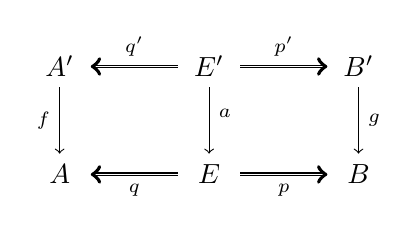
\begin{tikzpicture}[x=1.5em,y=1.5em]
  \node (Ap) at (0,1.3)    {$A'$};
  \node (Ep) at (3.6,1.3)  {$E'$};
  \node (Bp) at (7.2,1.3)  {$B'$};
  \node (A)  at (0,-1.3)   {$A$};
  \node (E)  at (3.6,-1.3) {$E$};
  \node (B)  at (7.2,-1.3) {$B$};
  \draw[double,->] (2.85,1.3) -- node[above]{$\scriptstyle q'$} (0.75,1.3);
  \draw[double,->] (4.35,1.3) -- node[above]{$\scriptstyle p'$} (6.45,1.3);
  \draw[double,->] (2.85,-1.3) -- node[below]{$\scriptstyle q$} (0.75,-1.3);
  \draw[double,->] (4.35,-1.3) -- node[below]{$\scriptstyle p$} (6.45,-1.3);
  \draw[->] (0,0.8) -- node[left]{$\scriptstyle f$} (0,-0.8);
  \draw[->] (3.6,0.8) -- node[right,pos=0.4]{$\scriptstyle a$} (3.6,-0.8);
  \draw[->] (7.2,0.8) -- node[right]{$\scriptstyle g$} (7.2,-0.8);
\end{tikzpicture}
\end{center}
其中两支这样的\trFunctor{} $a$ 与 $a'$ 被视为等价的，当存在自然同构
$\gamma\colon a\cong a'$ 使得 $q\gamma=\mathrm{id}_{aq'}$ 且
$p\gamma=\mathrm{id}_{bp'}$。
\end{definition}

\begin{observation}\label{obs:functor-space-over-product}
在\trModule{}或双侧等价纤维化的情形，从 $E'$ 到 $E$ 的、位于 $f\times g$
之上的映射所构成的\trFunctorSpace{} $\Fun_{f\times g}(E',E)$ 由如下\trPullback%
定义
\begin{center}
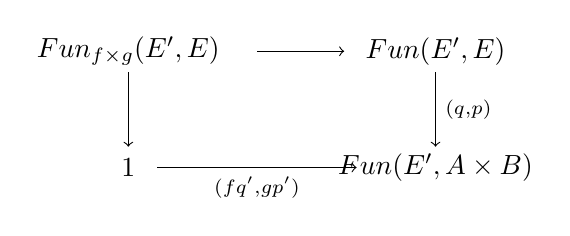
\begin{tikzpicture}[x=1.5em,y=1.5em]
  \node (Fl)  at (0,1.4)    {$\Fun_{f\times g}(E',E)$};
  \node (Ft)  at (7.4,1.4)  {$\Fun(E',E)$};
  \node (one) at (0,-1.4)   {$1$};
  \node (Fb)  at (7.4,-1.4) {$\Fun(E',A\times B)$};
  \draw[->] (3.1,1.4) -- (5.2,1.4);
  \draw[->] (7.4,0.9) -- node[right]{$\scriptstyle(q,p)$} (7.4,-0.9);
  \draw[->] (0,0.9) -- (0,-0.9);
  \draw[->] (0.7,-1.4) -- node[below]{$\scriptstyle(fq',gp')$} (5.5,-1.4);
  \node at (0.6,0.72) {$\scriptstyle\lrcorner$};
\end{tikzpicture}
\end{center}
正如在\cref{obs:one-categories-of-modules}中那样，模映射定义为该%
\trFunctorSpace{}中对象的\trIsomorphism{}类。
\end{observation}

现在我们引入双侧等价纤维化的\trDoubleCategory{}。这一结构既可以视为呈现于一个∞-宇宙
的\trHomotopyTwoCategory{} $\mathfrak{h}\mathcal{K}$ 中的诸数据之汇集，也
可以视为\cref{ex:cosmos-of-two-sided-isofibrations}所描述的那些以%
\trQuasiCategory{}富集的结构的商。
在某种意义上，后一观点更为自然，因为其水平复合由一个严格的\trUniversalProperty%
刻画，且不要求任何映射的同构类；但 2-范畴式的进路更为人熟悉，并且为发展%
\trInfinityCategories{}的形式范畴论提供了一个便利的舞台。

\begin{proposition}[双侧等价纤维化的\trDoubleCategory]%
\label{prop:double-category-of-two-sided-isofibrations}
一个∞-宇宙 $\mathcal{K}$ 的\trHomotopyTwoCategory{}承载一个（非幺的）%
\textbf{双侧等价纤维化的\trDoubleCategory}（double category of two-sided
isofibrations），其中：
\begin{itemize}
\item \textbf{对象}为\trInfinityCategories{}；
\item \textbf{竖直箭头}为\trFunctor{}；
\item \textbf{水平箭头} $A\xrightarrow{E}B$ 是双侧等价纤维化
$A\overset{q}{\twoheadleftarrow}E\overset{p}{\twoheadrightarrow}B$；并且
\item 以如下方块为边界的\textbf{\trCell}
\begin{center}
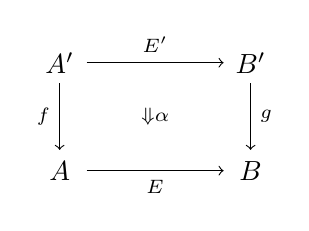
\begin{tikzpicture}[x=1.5em,y=1.5em]
  \node (Ap) at (0,1.3)    {$A'$};
  \node (Bp) at (4.6,1.3)  {$B'$};
  \node (A)  at (0,-1.3)   {$A$};
  \node (B)  at (4.6,-1.3) {$B$};
  \draw[->] (0.65,1.3) -- node[above]{$\scriptstyle E'$} (3.95,1.3);
  \draw[->] (0.65,-1.3) -- node[below]{$\scriptstyle E$} (3.95,-1.3);
  \draw[->] (0,0.8) -- node[left]{$\scriptstyle f$} (0,-0.8);
  \draw[->] (4.6,0.8) -- node[right]{$\scriptstyle g$} (4.6,-0.8);
  \node at (2.3,0) {$\scriptstyle\Downarrow\alpha$};
\end{tikzpicture}
\end{center}
是位于 $f\times g$ 上的双侧等价纤维化之间的映射；等价地，是\trQuasiCategory%
$\Fun_{f\times g}(E',E)$ 中对象的\trIsomorphism{}类。
\end{itemize}
\end{proposition}

\begin{proof}
箭头与胞腔的竖直复合即 $\mathcal{K}$ 中的复合。水平箭头的复合由命题 7.2.6
定义，而胞腔的水平复合由练习 7.2.i 定义。
由 $\mathcal{K}$ 中\trPullback{}与复合的\trSimplicial{}函子性，这两个构造
在典范自然同构的意义下都是结合的。
\end{proof}

刚才引入的这个\trDoubleCategory{}并不包含水平的单位箭头。出于技术上的原因，我们发现
把它们略去最为便利。

\begin{remark}[水平单位为何缺席]\label{rem:missing-horizontal-unit}
命题 7.2.6 所定义的跨度复合运算的单位是恒同跨度，而后者通常不是一条%
\trTwoSidedIsofibration{}。
与其把水平单位形式地添加到\cref{prop:double-category-of-two-sided-isofibrations}
的「\trDoubleCategory」之上，我们发现将它们略去更少引起混淆：因为当我们限制到最令我们
感兴趣的结构——模的\trVirtualEquipment——之上时，我们将看到，%
\trArrowInfinityCategory{}扮演着复合的水平单位这一角色，其意义将在命题
8.2.4 中得到描述，尽管对于跨度复合运算而言它并不定义一个水平复合单位。
\end{remark}

由练习 7.4.ii，\trModule{}在跨度复合之下并不构成\trDoubleCategory{}，这促使我们去寻找
另一种范畴结构来公理化它们的行为。
\trVirtualDoubleCategory{}是\trDoubleCategory{}的一种多范畴式类似物，适用于水平复合与单位可有可无的
场合。这一概念曾被 Burroni $[24]$ 与 Leinster $[76]$ 以各种名称研究过；
我们采用的是 Cruttwell 与 Shulman $[32]$ 的术语与记号。

\begin{definition}[\trVirtualDoubleCategory]\label{def:virtual-double-category}
一个\textbf{\trVirtualDoubleCategory}（virtual double category）由下列诸项构成：
\begin{itemize}
\item 一个由\textbf{对象}与\textbf{竖直箭头}构成的\trCategory{}；
\item 对任意一对对象 $A$、$B$，一个由\textbf{水平箭头} $A\to B$ 组成的
汇集；
\item 诸\textbf{\trCell}，其边界描绘如下
\begin{rveq}\label{eq:virtual-cell-boundary}
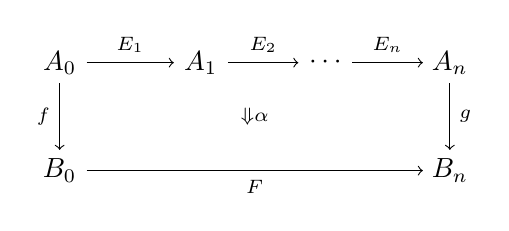
\begin{tikzpicture}[x=1.5em,y=1.5em]
  \node (A0) at (0,1.3)    {$A_{0}$};
  \node (A1) at (3.4,1.3)  {$A_{1}$};
  \node (Ad) at (6.4,1.3)  {$\cdots$};
  \node (An) at (9.4,1.3)  {$A_{n}$};
  \node (B0) at (0,-1.3)   {$B_{0}$};
  \node (Bn) at (9.4,-1.3) {$B_{n}$};
  \draw[->] (0.65,1.3) -- node[above]{$\scriptstyle E_{1}$} (2.75,1.3);
  \draw[->] (4.05,1.3) -- node[above]{$\scriptstyle E_{2}$} (5.75,1.3);
  \draw[->] (7.05,1.3) -- node[above]{$\scriptstyle E_{n}$} (8.75,1.3);
  \draw[->] (0,0.8) -- node[left]{$\scriptstyle f$} (0,-0.8);
  \draw[->] (9.4,0.8) -- node[right]{$\scriptstyle g$} (9.4,-0.8);
  \node at (4.7,0) {$\scriptstyle\Downarrow\alpha$};
  \draw[->] (0.65,-1.3) -- node[below]{$\scriptstyle F$} (8.75,-1.3);
\end{tikzpicture}
\end{rveq}
——包括在 $A_{0}=A_{n}$ 的情形下那些水平源长度为零的胞腔；
\item 对任何如下左图所示的构型，一个如下右图所示的\textbf{复合胞腔}
（composite cell）
\begin{rveq}\label{eq:virtual-composite-cell}
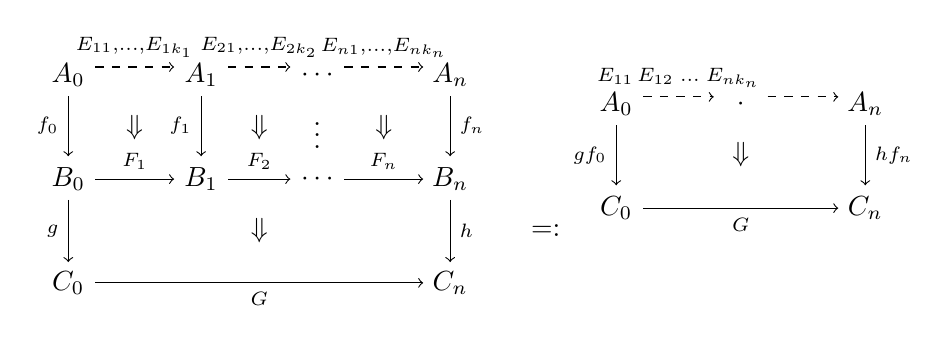
\begin{tikzpicture}[x=1.5em,y=1.5em]
  \node (A0) at (0,3.1)   {$A_{0}$};
  \node (A1) at (3.2,3.1) {$A_{1}$};
  \node (Ad) at (6.0,3.1) {$\cdots$};
  \node (An) at (9.2,3.1) {$A_{n}$};
  \draw[->,dashed] (0.65,3.3) -- node[above]{$\scriptstyle E_{11},\ldots,E_{1k_{1}}$} (2.55,3.3);
  \draw[->,dashed] (3.85,3.3) -- node[above]{$\scriptstyle E_{21},\ldots,E_{2k_{2}}$} (5.35,3.3);
  \draw[->,dashed] (6.65,3.3) -- node[above]{$\scriptstyle E_{n1},\ldots,E_{nk_{n}}$} (8.55,3.3);
  \draw[->] (0,2.6) -- node[left]{$\scriptstyle f_{0}$} (0,1.15);
  \draw[->] (3.2,2.6) -- node[left]{$\scriptstyle f_{1}$} (3.2,1.15);
  \node at (6.0,1.85) {$\vdots$};
  \draw[->] (9.2,2.6) -- node[right]{$\scriptstyle f_{n}$} (9.2,1.15);
  \node at (1.6,1.85) {$\Downarrow$};
  \node at (4.6,1.85) {$\Downarrow$};
  \node at (7.6,1.85) {$\Downarrow$};
  \node (B0) at (0,0.6)   {$B_{0}$};
  \node (B1) at (3.2,0.6) {$B_{1}$};
  \node (Bd) at (6.0,0.6) {$\cdots$};
  \node (Bn) at (9.2,0.6) {$B_{n}$};
  \draw[->] (0.65,0.6) -- node[above]{$\scriptstyle F_{1}$} (2.55,0.6);
  \draw[->] (3.85,0.6) -- node[above]{$\scriptstyle F_{2}$} (5.35,0.6);
  \draw[->] (6.65,0.6) -- node[above]{$\scriptstyle F_{n}$} (8.55,0.6);
  \draw[->] (0,0.1) -- node[left]{$\scriptstyle g$} (0,-1.4);
  \draw[->] (9.2,0.1) -- node[right]{$\scriptstyle h$} (9.2,-1.4);
  \node at (4.6,-0.65) {$\Downarrow$};
  \node (C0) at (0,-1.9)  {$C_{0}$};
  \node (Cn) at (9.2,-1.9){$C_{n}$};
  \draw[->] (0.65,-1.9) -- node[below]{$\scriptstyle G$} (8.55,-1.9);
  \node at (11.5,-0.65) {$=:$};
  \begin{scope}[shift={(13.2,0)}]
  \node (a0) at (0,2.4)   {$A_{0}$};
  \node (ad) at (3.0,2.4) {$\cdot$};
  \node (an) at (6.0,2.4) {$A_{n}$};
  \draw[->,dashed] (0.65,2.58) --
    node[above,pos=0.5]{$\scriptstyle E_{11}\,E_{12}\;\ldots\;E_{nk_{n}}$} (2.35,2.58);
  \draw[->,dashed] (3.65,2.58) -- (5.35,2.58);
  \draw[->] (0,1.9) -- node[left]{$\scriptstyle gf_{0}$} (0,0.45);
  \draw[->] (6.0,1.9) -- node[right]{$\scriptstyle hf_{n}$} (6.0,0.45);
  \node at (3.0,1.2) {$\Downarrow$};
  \node (c0) at (0,-0.1)  {$C_{0}$};
  \node (cn) at (6.0,-0.1){$C_{n}$};
  \draw[->] (0.65,-0.1) -- node[below]{$\scriptstyle G$} (5.35,-0.1);
  \end{scope}
\end{tikzpicture}
\end{rveq}
\item 对每一支水平箭头，一个\textbf{恒同胞腔}（identity cell）
\begin{center}
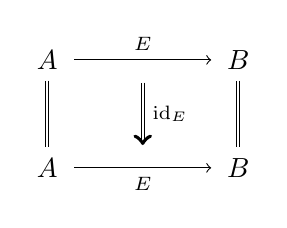
\begin{tikzpicture}[x=1.5em,y=1.5em]
  \node (At) at (0,1.3)    {$A$};
  \node (Bt) at (4.6,1.3)  {$B$};
  \node (Ab) at (0,-1.3)   {$A$};
  \node (Bb) at (4.6,-1.3) {$B$};
  \draw[->] (0.65,1.3) -- node[above]{$\scriptstyle E$} (3.95,1.3);
  \draw[->] (0.65,-1.3) -- node[below]{$\scriptstyle E$} (3.95,-1.3);
  \draw[double] (0,0.8) -- (0,-0.8);
  \draw[double] (4.6,0.8) -- (4.6,-0.8);
  \draw[double,->] (2.3,0.75) -- node[right]{$\scriptstyle\mathrm{id}_{E}$} (2.3,-0.75);
\end{tikzpicture}
\end{center}
\end{itemize}
使得胞腔的复合在通常的多范畴意义下既是结合的又是幺的。
\end{definition}

\begin{lemma}\label{lem:virtual-double-category-of-two-sided-isofibrations}
存在一个双侧等价纤维化的\trVirtualDoubleCategory{}，其中：
\begin{itemize}
\item \textbf{对象}为\trInfinityCategories{}；
\item \textbf{竖直箭头}为\trFunctor{}；
\item \textbf{水平箭头}为双侧等价纤维化；并且
\item $n$ 元\textbf{\trCell}（\eqref{eq:virtual-cell-boundary}）是位于
$f\times g$ 之上的双侧等价纤维化之间的映射
\begin{rveq}\label{eq:n-ary-cell-as-map}
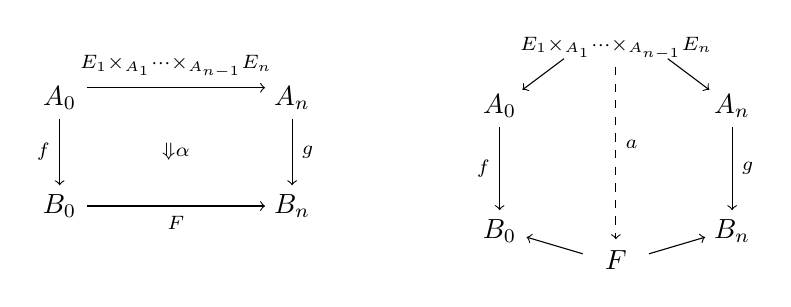
\begin{tikzpicture}[x=1.5em,y=1.5em]
  \node (A0) at (0,1.3)    {$A_{0}$};
  \node (An) at (5.6,1.3)  {$A_{n}$};
  \draw[->] (0.65,1.55) --
    node[above]{$\scriptstyle E_{1}\times_{A_{1}}\cdots\times_{A_{n-1}}E_{n}$} (4.95,1.55);
  \node (B0) at (0,-1.3)   {$B_{0}$};
  \node (Bn) at (5.6,-1.3) {$B_{n}$};
  \draw[->] (0,0.8) -- node[left]{$\scriptstyle f$} (0,-0.8);
  \draw[->] (5.6,0.8) -- node[right]{$\scriptstyle g$} (5.6,-0.8);
  \node at (2.8,0) {$\scriptstyle\Downarrow\alpha$};
  \draw[->] (0.65,-1.3) -- node[below]{$\scriptstyle F$} (4.95,-1.3);
  \node at (7.9,0) {$\leftrightsquigarrow$};
  \begin{scope}[shift={(10.6,0)}]
  \node (P) at (2.8,2.5)
    {$\scriptstyle E_{1}\times_{A_{1}}\cdots\times_{A_{n-1}}E_{n}$};
  \node (a0) at (0,1.1)   {$A_{0}$};
  \node (an) at (5.6,1.1) {$A_{n}$};
  \draw[->] (1.55,2.25) -- (0.55,1.5);
  \draw[->] (4.05,2.25) -- (5.05,1.5);
  \draw[->,dashed] (2.8,2.05) -- node[right,pos=0.45]{$\scriptstyle a$} (2.8,-2.1);
  \node (b0) at (0,-1.9)   {$B_{0}$};
  \node (bn) at (5.6,-1.9) {$B_{n}$};
  \draw[->] (0,0.6) -- node[left]{$\scriptstyle f$} (0,-1.4);
  \draw[->] (5.6,0.6) -- node[right]{$\scriptstyle g$} (5.6,-1.4);
  \node (F) at (2.8,-2.6) {$F$};
  \draw[->] (2.0,-2.45) -- (0.65,-2.05);
  \draw[->] (3.6,-2.45) -- (4.95,-2.05);
  \end{scope}
\end{tikzpicture}
\end{rveq}
其唯一的竖直源是 \eqref{eq:virtual-cell-boundary} 中构成其水平源\footnote{%
原书两处均印作「vertical」：此处作「comprising the vertical source in
(8.1.9)」（构成 (8.1.9) 中竖直源的……），零元段作「which have an empty
sequence as their vertical domain」（以空序列为其竖直定义域）。按定义
8.1.8，(8.1.9) 中那列跨度构成胞腔的水平源、空序列构成零元胞腔的水平%
定义域（对照原书 p.313 平行句「comprising the horizontal source in the
left-hand diagram」即作 horizontal），疑两处「vertical」均为
「horizontal」之排印误，此处一并径改。——译者注}的那列跨度的 $(n-1)$ 重跨度复合。
\end{itemize}
\end{lemma}

\begin{proof}
所需的诸复合定律可以这样定义：把诸\trVirtualDoubleCategory{}嵌入到%
\cref{prop:double-category-of-two-sided-isofibrations}的诸\trDoubleCategory{}之中。
例如，\eqref{eq:virtual-composite-cell} 左侧所示的那个构型，其复合可以
定义为：先在等价纤维化的\trDoubleCategory{}中把顶部的 $k$ 支胞腔作水平复合，再把结果
与底部的胞腔作竖直复合。其结果即\trVirtualDoubleCategory{}中一支形状正确的
$k_{1}+\cdots+k_{n}$ 元胞腔。

尚待定义的只是零元胞腔\footnote{注意记号 $\rvnullpair$ 之使用：它表示
一支零元胞腔的零元源；采用这一记号，是为了让此类胞腔得以自然地纳入虚拟%
\trDoubleCategory{}中诸胞腔的\trPastingDiagram{}。}
——即以空序列为其水平定义域的那些胞腔
\begin{center}
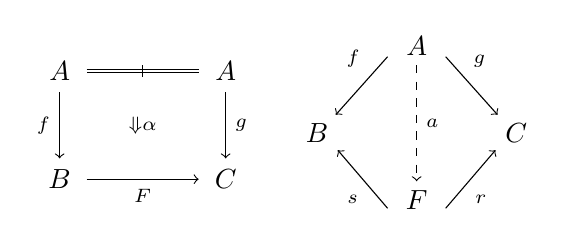
\begin{tikzpicture}[x=1.5em,y=1.5em]
  \node (At) at (0,1.3)   {$A$};
  \node (At2) at (4.0,1.3){$A$};
  \node (B)  at (0,-1.3)  {$B$};
  \node (C)  at (4.0,-1.3){$C$};
  \draw[double] (0.65,1.3) -- (3.35,1.3);
  \draw (2.0,1.45) -- (2.0,1.15);
  \draw[->] (0.65,-1.3) -- node[below]{$\scriptstyle F$} (3.35,-1.3);
  \draw[->] (0,0.8) -- node[left]{$\scriptstyle f$} (0,-0.8);
  \draw[->] (4.0,0.8) -- node[right]{$\scriptstyle g$} (4.0,-0.8);
  \node at (2.0,0) {$\scriptstyle\Downarrow\alpha$};
  \node at (6.3,0) {$\leftrightsquigarrow$};
  \begin{scope}[shift={(8.6,0)}]
  \node (nA) at (0,1.9)    {$A$};
  \node (nB) at (-2.4,-0.2){$B$};
  \node (nC) at (2.4,-0.2) {$C$};
  \draw[->] (-0.7,1.65) -- node[above left,pos=0.35]{$\scriptstyle f$} (-1.95,0.25);
  \draw[->] (0.7,1.65)  -- node[above right,pos=0.35]{$\scriptstyle g$} (1.95,0.25);
  \draw[->,dashed] (0,1.45) -- node[right,pos=0.5]{$\scriptstyle a$} (0,-1.35);
  \node (nF) at (0,-1.8) {$F$};
  \draw[->] (-0.7,-2.0) -- node[below left,pos=0.4]{$\scriptstyle s$} (-1.9,-0.6);
  \draw[->] (0.7,-2.0)  -- node[below right,pos=0.4]{$\scriptstyle r$} (1.9,-0.6);
  \end{scope}
\end{tikzpicture}
\end{center}
我们把它解读为一个 0 重拉回，这即是从 $A$ 到 $A$ 的恒同跨度。于是，上方
左图所展示的零元胞腔是上方右图所示诸映射的纤维化同构类，其中 $a$ 与 $a'$
位于同一个等价类中，当存在自然同构 $\gamma\colon a\cong a'$ 使得
$s\gamma=\mathrm{id}_{f}$ 且 $r\gamma=\mathrm{id}_{g}$。
\end{proof}

\begin{remark}\label{rem:diagonal-nullary-morphism}
例如，映射
\begin{center}
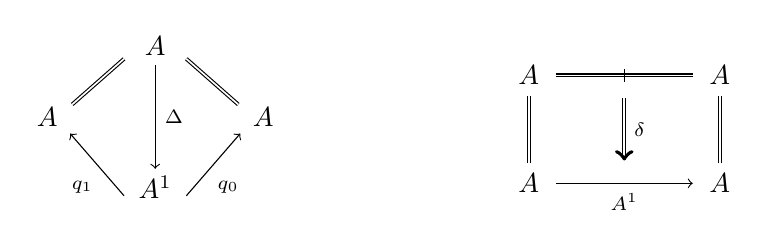
\begin{tikzpicture}[x=1.5em,y=1.5em]
  \begin{scope}[shift={(0,0)}]
  \node (At) at (0,2.0)    {$A$};
  \node (Al) at (-2.6,0.3) {$A$};
  \node (Ar) at (2.6,0.3)  {$A$};
  \node (Ab) at (0,-1.4)   {$A^{\mathbb{1}}$};
  \draw[double] (-0.75,1.7) -- (-2.0,0.6);
  \draw[double] (0.75,1.7)  -- (2.0,0.6);
  \draw[->] (0,1.55) -- node[right,pos=0.5]{$\scriptstyle\Delta$} (0,-0.95);
  \draw[->] (-0.75,-1.6) -- node[below left,pos=0.4]{$\scriptstyle q_{1}$} (-2.05,-0.1);
  \draw[->] (0.75,-1.6)  -- node[below right,pos=0.4]{$\scriptstyle q_{0}$} (2.05,-0.1);
  \end{scope}
  \node at (5.4,0.2) {$\leftrightsquigarrow$};
  \begin{scope}[shift={(9.0,0)}]
  \node (a) at (0,1.3)    {$A$};
  \node (b) at (4.6,1.3)  {$A$};
  \node (c) at (0,-1.3)   {$A$};
  \node (d) at (4.6,-1.3) {$A$};
  \draw[double] (0.65,1.3) -- (3.95,1.3);
  \draw (2.3,1.45) -- (2.3,1.15);
  \draw[->] (0.65,-1.3) -- node[below]{$\scriptstyle A^{\mathbb{1}}$} (3.95,-1.3);
  \draw[double] (0,0.8) -- (0,-0.8);
  \draw[double] (4.6,0.8) -- (4.6,-0.8);
  \draw[double,->] (2.3,0.75) -- node[right]{$\scriptstyle\delta$} (2.3,-0.75);
  \end{scope}
\end{tikzpicture}
\end{center}
在双侧等价纤维化的\trVirtualDoubleCategory{}中定义了一个余定义域为
$A\xrightarrow{A^{\mathbb{1}}}A$ 的零元态射。然而请注意：尽管
$\Delta\colon A\simeq A^{\mathbb{1}}$ 在周围的∞-宇宙中定义了一个%
\trEquivalence{}，这个胞腔在任何一种\trVirtualDoubleCategory{}中都不定义\trIsomorphism{}。
这一零元态射赋予 $A\xrightarrow{A^{\mathbb{1}}}A$ 一种适合\trVirtualDoubleCategory{}的
单位结构（见练习 8.2.iii）。正是因为这类原因，我们在%
\cref{prop:double-category-of-two-sided-isofibrations}中略去了水平的恒同
箭头。
\end{remark}

我们感兴趣的主要例子，是一个通过限制水平箭头的类、并取其之间的全部胞腔
而定义的全子\trVirtualDoubleCategory{}。
由于\trVirtualDoubleCategory{}的结构中给出的运算仅有竖直源与竖直靶、竖直恒同以及竖直
复合，显然这一子结构在这些运算之下全部封闭，从而继承\trVirtualDoubleCategory{}的结构。

\begin{corollary}\label{cor:virtual-double-category-of-modules}
对任意∞-宇宙 $\mathcal{K}$，存在一个\trModule{}的\trVirtualDoubleCategory
$\Mod(\mathcal{K})$，它定义为等价纤维化的\trVirtualDoubleCategory{}的一个全子范畴，其中：
\begin{itemize}
\item \textbf{对象}为\trInfinityCategories{}；
\item \textbf{竖直箭头}为\trFunctor{}；
\item \textbf{水平箭头} $A\xrightarrow{E}B$ 是从 $A$ 到 $B$ 的\trModule{}
$E$；
\item $n$ 元\textbf{\trCell}是位于 $f\times g$ 之上的、双侧等价纤维化之间
的映射的纤维化同构类：
\begin{rveq}\label{eq:n-ary-module-map}
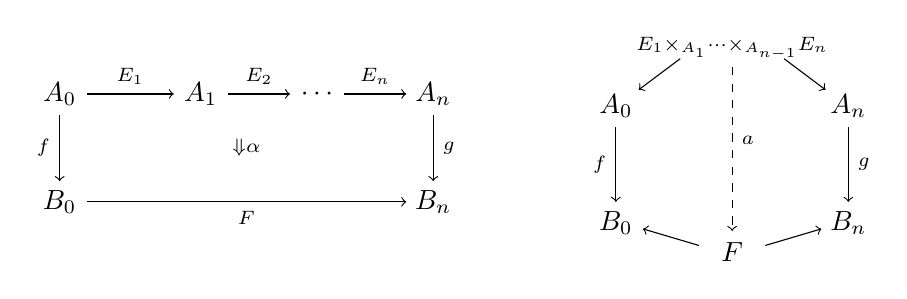
\begin{tikzpicture}[x=1.5em,y=1.5em]
  \node (A0) at (0,1.3)    {$A_{0}$};
  \node (A1) at (3.4,1.3)  {$A_{1}$};
  \node (Ad) at (6.2,1.3)  {$\cdots$};
  \node (An) at (9.0,1.3)  {$A_{n}$};
  \draw[->] (0.65,1.3) -- node[above]{$\scriptstyle E_{1}$} (2.75,1.3);
  \draw[->] (4.05,1.3) -- node[above]{$\scriptstyle E_{2}$} (5.55,1.3);
  \draw[->] (6.85,1.3) -- node[above]{$\scriptstyle E_{n}$} (8.35,1.3);
  \node (B0) at (0,-1.3)   {$B_{0}$};
  \node (Bn) at (9.0,-1.3) {$B_{n}$};
  \draw[->] (0,0.8) -- node[left]{$\scriptstyle f$} (0,-0.8);
  \draw[->] (9.0,0.8) -- node[right]{$\scriptstyle g$} (9.0,-0.8);
  \node at (4.5,0) {$\scriptstyle\Downarrow\alpha$};
  \draw[->] (0.65,-1.3) -- node[below]{$\scriptstyle F$} (8.35,-1.3);
  \node at (11.3,0) {$\leftrightsquigarrow$};
  \begin{scope}[shift={(13.4,0)}]
  \node (P) at (2.8,2.4)
    {$\scriptstyle E_{1}\times_{A_{1}}\cdots\times_{A_{n-1}}E_{n}$};
  \node (a0) at (0,1.0)   {$A_{0}$};
  \node (an) at (5.6,1.0) {$A_{n}$};
  \draw[->] (1.55,2.15) -- (0.55,1.4);
  \draw[->] (4.05,2.15) -- (5.05,1.4);
  \draw[->,dashed] (2.8,1.95) -- node[right,pos=0.45]{$\scriptstyle a$} (2.8,-2.0);
  \node (b0) at (0,-1.8)   {$B_{0}$};
  \node (bn) at (5.6,-1.8) {$B_{n}$};
  \draw[->] (0,0.5) -- node[left]{$\scriptstyle f$} (0,-1.3);
  \draw[->] (5.6,0.5) -- node[right]{$\scriptstyle g$} (5.6,-1.3);
  \node (F) at (2.8,-2.5) {$F$};
  \draw[->] (2.0,-2.35) -- (0.65,-1.95);
  \draw[->] (3.6,-2.35) -- (4.95,-1.95);
  \end{scope}
\end{tikzpicture}
\end{rveq}
\end{itemize}
\end{corollary}

\eqref{eq:n-ary-module-map} 的\textbf{$n$ 元模映射}（n-ary module maps）
可以设想为\cref{lem:virtual-double-category-of-two-sided-isofibrations}
的 $n$ 元胞腔的特例，其中 $E_{1},\ldots,E_{n}$ 与 $F$ 全都被要求是%
\trModule{}：图表 \eqref{eq:n-ary-cell-as-map} 中那个唯一的水平源，是由左图
中构成水平源的那列\trModule{}经 $n-1$ 重\trPullback{}所定义的那条%
\trTwoSidedFibration{}。
我们把作为一支 $n$ 元模映射的水平定义域出现的那列有限的\trModule{}称为
一个\textbf{模的相容序列}（compatible sequence of modules）；这只意味着：
它们的水平源与水平靶以显见的方式相容。

下面这个特殊情形，给出了这种 $n$ 元模映射概念何以切题的一个暗示。

\begin{lemma}\label{lem:comma-module-maps-bijection}
在如下两类东西之间存在一个双射：其一，余定义域\trModule{}为下左图所示的
逗号\trModule{}的那些 $n$ 元模映射；其二，\trHomotopyTwoCategory{}中边界
为下右图所示的那些\trNaturalTransformation{}：
\begin{center}
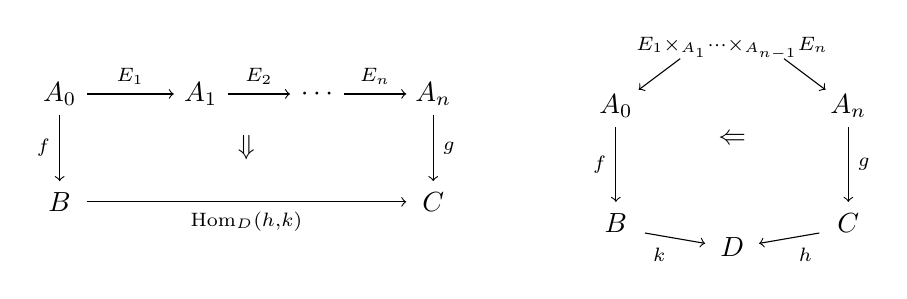
\begin{tikzpicture}[x=1.5em,y=1.5em]
  \node (A0) at (0,1.3)    {$A_{0}$};
  \node (A1) at (3.4,1.3)  {$A_{1}$};
  \node (Ad) at (6.2,1.3)  {$\cdots$};
  \node (An) at (9.0,1.3)  {$A_{n}$};
  \draw[->] (0.65,1.3) -- node[above]{$\scriptstyle E_{1}$} (2.75,1.3);
  \draw[->] (4.05,1.3) -- node[above]{$\scriptstyle E_{2}$} (5.55,1.3);
  \draw[->] (6.85,1.3) -- node[above]{$\scriptstyle E_{n}$} (8.35,1.3);
  \node (B) at (0,-1.3) {$B$};
  \node (C) at (9.0,-1.3){$C$};
  \draw[->] (0,0.8) -- node[left]{$\scriptstyle f$} (0,-0.8);
  \draw[->] (9.0,0.8) -- node[right]{$\scriptstyle g$} (9.0,-0.8);
  \node at (4.5,0) {$\Downarrow$};
  \draw[->] (0.65,-1.3) -- node[below]{$\scriptstyle\mathrm{Hom}_{D}(h,k)$} (8.35,-1.3);
  \node at (11.3,0) {$\leftrightsquigarrow$};
  \begin{scope}[shift={(13.4,0)}]
  \node (P) at (2.8,2.4)
    {$\scriptstyle E_{1}\times_{A_{1}}\cdots\times_{A_{n-1}}E_{n}$};
  \node (a0) at (0,1.0)   {$A_{0}$};
  \node (an) at (5.6,1.0) {$A_{n}$};
  \draw[->] (1.55,2.15) -- (0.55,1.4);
  \draw[->] (4.05,2.15) -- (5.05,1.4);
  \node at (2.8,0.2) {$\Leftarrow$};
  \node (b) at (0,-1.8)  {$B$};
  \node (d) at (2.8,-2.4){$D$};
  \node (c) at (5.6,-1.8){$C$};
  \draw[->] (0,0.5) -- node[left]{$\scriptstyle f$} (0,-1.3);
  \draw[->] (5.6,0.5) -- node[right]{$\scriptstyle g$} (5.6,-1.3);
  \draw[->] (0.7,-2.05) -- node[below left,pos=0.5]{$\scriptstyle k$} (2.15,-2.3);
  \draw[->] (4.9,-2.05) -- node[below right,pos=0.5]{$\scriptstyle h$} (3.45,-2.3);
  \end{scope}
\end{tikzpicture}
\end{center}
\end{lemma}

\begin{proof}
把\cref{def:maps-in-squares}与命题 3.4.7 结合起来。
\end{proof}

对于模的\trVirtualDoubleCategory{}中的任意一对对象 $A$ 与 $B$，存在一个竖直 1-范畴，其
对象为从 $A$ 到 $B$ 的\trModule{}、其态射为位于一对恒同\trFunctor{}之上的
模映射；这个范畴与\cref{obs:one-categories-of-modules}中引入的从 $A$ 到
$B$ 的模的 1-范畴相重合。在这一语境下，%
\cref{lem:one-category-equivalences}可以重述如下：

\begin{lemma}\label{lem:module-vertical-isomorphism}
一对平行的\trModule{} $A\xrightarrow{E}B$ 与 $A\xrightarrow{F}B$ 作为模的%
\trVirtualDoubleCategory{}中模的竖直 1-范畴的对象而同构，当且仅当
$E\simeq_{A\times B}F$。
\end{lemma}

为了与全书其余部分保持一致，凡当\trModule{} $A\xrightarrow{E}B$ 与
$A\xrightarrow{F}B$ 作为从 $A$ 到 $B$ 的模的竖直 1-范畴中的对象同构时，
我们就写作 $E\simeq F$ 或 $E\simeq_{A\times B}F$。例如，命题 4.1.1 证明：
一个\trFunctor{} $f\colon B\to A$ 作为一个\trFunctor{} $u\colon A\to B$
的\trLeftAdjoint{}，当且仅当
$\mathrm{Hom}_{A}(f,A)\simeq_{A\times B}\mathrm{Hom}_{B}(B,u)$；也就是说，
当且仅当诸\trModule{} $A\xrightarrow{\mathrm{Hom}_{A}(f,A)}B$\footnote{%
原书印作「$B\xrightarrow{\mathrm{Hom}_{A}(f,A)}A$」。按本书模的方向约定
（第 7 章定义 7.4.7：$\mathrm{Hom}_{B}(B,f)$ 是从 $A$ 到 $B$ 的模），%
$\mathrm{Hom}_{A}(f,A)$ 应为从 $A$ 到 $B$ 的模，且与本句末「从 $A$ 到
$B$ 的模的竖直 1-范畴」相合；第一支模疑为
「$A\xrightarrow{\mathrm{Hom}_{A}(f,A)}B$」之误，此处径改。——译者注}
与 $A\xrightarrow{\mathrm{Hom}_{B}(B,u)}B$ 作为从 $A$ 到 $B$ 的模的竖直
1-范畴中的对象同构。

\subsection*{练习}

\begin{exercise}\label{ex:cosmos-of-two-sided-isofibrations}
由练习 6.1.iii，对任意∞-宇宙 $\mathcal{K}$，存在一个∞-宇宙
$\mathcal{K}^{\times}$，其对象为任意一对∞-范畴之间的双侧等价纤维化——
这些恰好是由该\trSpan{}所标引的「\trFibrant{}图表」，其中该\trSpan{}被
视为一个逆范畴。
请把这个∞-宇宙连同诸端点求值\trFunctor{}
$\mathcal{K}^{\times}\to\mathcal{K}$ 一起使用，给出双侧等价纤维化的\trDoubleCategory
的第二个描述——把它描述为在∞-宇宙、\trCosmologicalFunctor{}与%
\trSimplicial{}自然同构的层面上定义的一个非幺内范畴的商。\footnote{我们
认为下述问题是一个未决问题：在双侧等价纤维化的非幺\trDoubleCategory{}或模的虚拟双
范畴上安置一个「双重拟范畴」是否有用。}
\end{exercise}

\begin{exercise}\label{ex:double-defines-virtual}
证明：任何\trDoubleCategory{}都定义一个\trVirtualDoubleCategory{}。\footnote{若该\trDoubleCategory{}缺乏水平的恒同
态射，则相应的\trVirtualDoubleCategory{}可能缺乏零元态射——除非这些态射能够以某种别的
方式定义，正如我们在\cref{lem:virtual-double-category-of-two-sided-isofibrations}
的证明中所做的那样。}
\end{exercise}

\begin{exercise}\label{ex:three-bijections-from-yoneda}
用定理 7.4.8 的三条陈述，描述模的\trVirtualDoubleCategory{}中具有各种边界形状的胞腔之间
的三个双射。
\end{exercise}

\begin{exercise}\label{ex:map-of-two-sided-fibrations}
设 $A\overset{q}{\twoheadleftarrow}E\overset{p}{\twoheadrightarrow}B$ 与
$A\overset{s}{\twoheadleftarrow}F\overset{r}{\twoheadrightarrow}B$ 是两条%
\trTwoSidedFibration{}。从
$A\overset{q}{\twoheadleftarrow}E\overset{p}{\twoheadrightarrow}B$ 到
$A\overset{s}{\twoheadleftarrow}F\overset{r}{\twoheadrightarrow}B$ 的一支%
\textbf{双侧纤维化映射}（map of two-sided fibrations），是一个由严格交换
的\trFunctor{} $a$ 构成的纤维化同构类，使得左方形在诸%
\trCocartesianFibration{}之间定义一个\trCartesianFunctor{}，而右方形在诸%
\trCartesianFibration{}之间定义一个\trCartesianFunctor{}（见命题 7.1.7）。
\begin{center}
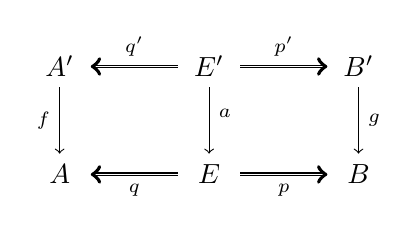
\begin{tikzpicture}[x=1.5em,y=1.5em]
  \node (Ap) at (0,1.3)    {$A'$};
  \node (Ep) at (3.6,1.3)  {$E'$};
  \node (Bp) at (7.2,1.3)  {$B'$};
  \node (A)  at (0,-1.3)   {$A$};
  \node (E)  at (3.6,-1.3) {$E$};
  \node (B)  at (7.2,-1.3) {$B$};
  \draw[double,->] (2.85,1.3) -- node[above]{$\scriptstyle q'$} (0.75,1.3);
  \draw[double,->] (4.35,1.3) -- node[above]{$\scriptstyle p'$} (6.45,1.3);
  \draw[double,->] (2.85,-1.3) -- node[below]{$\scriptstyle q$} (0.75,-1.3);
  \draw[double,->] (4.35,-1.3) -- node[below]{$\scriptstyle p$} (6.45,-1.3);
  \draw[->] (0,0.8) -- node[left]{$\scriptstyle f$} (0,-0.8);
  \draw[->] (3.6,0.8) -- node[right,pos=0.4]{$\scriptstyle a$} (3.6,-0.8);
  \draw[->] (7.2,0.8) -- node[right]{$\scriptstyle g$} (7.2,-0.8);
\end{tikzpicture}
\end{center}
请定义一个双侧纤维化的\trDoubleCategory{}：作为\cref{prop:double-category-of-two-sided-isofibrations}
的双侧等价纤维化\trDoubleCategory{}的一个非全子范畴。
\end{exercise}

   %
\providecommand{\Mod}{\mathbb{M}od}
\providecommand{\HomA}{\mathrm{Hom}_{A}}
\providecommand{\Fun}{\operatorname{Fun}}

\section{模的虚拟装备}\label{sec:virtual-equipment-of-modules}

\trInfinityCosmos{} $\mathcal{K}$ 中的模的\trVirtualDoubleCategory $\Mod(\mathcal{K})$ 具有%
刻画一个\emph{\trVirtualEquipment}（virtual equipment）的两个特殊性质。在陈述%
定义之前，我们先逐一考察它们。

\begin{proposition}[限制]\label{prop:restriction}
$\Mod(\mathcal{K})$ 中任何如下左图所示的图表皆可补全为一个\textbf{\trCartesian%
\trCell}（cartesian cell），如下右图所示
\begin{center}
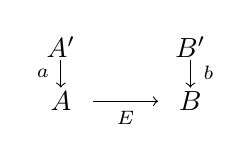
\begin{tikzpicture}[x=1.3em,y=1.3em]
  \node at (0,1.5) {$A'$};
  \node at (3.6,1.5) {$B'$};
  \node at (0,0) {$A$};
  \node at (3.6,0) {$B$};
  \draw[->] (0,1.15) -- (0,0.38);
  \node at (-0.5,0.78) {$\scriptstyle a$};
  \draw[->] (3.6,1.15) -- (3.6,0.38);
  \node at (4.1,0.78) {$\scriptstyle b$};
  \draw[->] (0.9,0) -- (2.7,0);
  \node at (1.8,-0.45) {$\scriptstyle E$};
\end{tikzpicture}
\qquad$\rightsquigarrow$\qquad
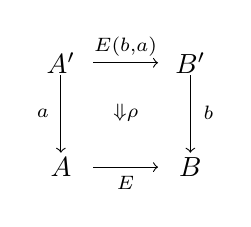
\begin{tikzpicture}[x=1.3em,y=1.3em]
  \node at (0,2.9) {$A'$};
  \node at (3.6,2.9) {$B'$};
  \node at (0,0) {$A$};
  \node at (3.6,0) {$B$};
  \draw[->] (0.9,2.9) -- (2.7,2.9);
  \node at (1.8,3.35) {$\scriptstyle E(b,a)$};
  \draw[->] (0,2.55) -- (0,0.4);
  \node at (-0.5,1.5) {$\scriptstyle a$};
  \draw[->] (3.6,2.55) -- (3.6,0.4);
  \node at (4.1,1.5) {$\scriptstyle b$};
  \node at (1.8,1.5) {$\scriptstyle\Downarrow\rho$};
  \draw[->] (0.9,0) -- (2.7,0);
  \node at (1.8,-0.45) {$\scriptstyle E$};
\end{tikzpicture}
\end{center}
并由如下\trUniversalProperty{}刻画：如下左图所示的任何胞腔都经由 $\rho$ 唯一地%
分解，如下右图所示：
\begin{center}
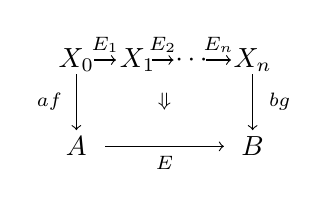
\begin{tikzpicture}[x=1.3em,y=1.3em]
  \node at (0,3) {$X_{0}$};
  \node at (1.7,3) {$X_{1}$};
  \node at (3.2,3) {$\cdots$};
  \node at (4.9,3) {$X_{n}$};
  \draw[->] (0.5,3) -- (1.1,3);
  \node at (0.8,3.42) {$\scriptstyle E_{1}$};
  \draw[->] (2.1,3) -- (2.7,3);
  \node at (2.4,3.42) {$\scriptstyle E_{2}$};
  \draw[->] (3.6,3) -- (4.3,3);
  \node at (3.95,3.42) {$\scriptstyle E_{n}$};
  \node at (0,0.6) {$A$};
  \node at (4.9,0.6) {$B$};
  \draw[->] (0,2.6) -- (0,1.05);
  \node at (-0.75,1.85) {$\scriptstyle af$};
  \draw[->] (4.9,2.6) -- (4.9,1.05);
  \node at (5.65,1.85) {$\scriptstyle bg$};
  \node at (2.45,1.85) {$\scriptstyle\Downarrow$};
  \draw[->] (0.8,0.6) -- (4.1,0.6);
  \node at (2.45,0.15) {$\scriptstyle E$};
\end{tikzpicture}
\qquad $:=$ \qquad
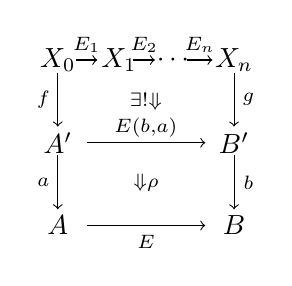
\begin{tikzpicture}[x=1.3em,y=1.3em]
  \node at (0,4.6) {$X_{0}$};
  \node at (1.7,4.6) {$X_{1}$};
  \node at (3.2,4.6) {$\cdots$};
  \node at (4.9,4.6) {$X_{n}$};
  \draw[->] (0.5,4.6) -- (1.1,4.6);
  \node at (0.8,5.02) {$\scriptstyle E_{1}$};
  \draw[->] (2.1,4.6) -- (2.7,4.6);
  \node at (2.4,5.02) {$\scriptstyle E_{2}$};
  \draw[->] (3.6,4.6) -- (4.3,4.6);
  \node at (3.95,5.02) {$\scriptstyle E_{n}$};
  \draw[->] (0,4.25) -- (0,2.75);
  \node at (-0.4,3.5) {$\scriptstyle f$};
  \node at (2.45,3.45) {$\scriptstyle\exists!\Downarrow$};
  \draw[->] (4.9,4.25) -- (4.9,2.75);
  \node at (5.3,3.5) {$\scriptstyle g$};
  \node at (0,2.3) {$A'$};
  \node at (4.9,2.3) {$B'$};
  \draw[->] (0.8,2.3) -- (4.1,2.3);
  \node at (2.45,2.72) {$\scriptstyle E(b,a)$};
  \draw[->] (0,1.95) -- (0,0.45);
  \node at (-0.4,1.2) {$\scriptstyle a$};
  \draw[->] (4.9,1.95) -- (4.9,0.45);
  \node at (5.3,1.2) {$\scriptstyle b$};
  \node at (2.45,1.2) {$\scriptstyle\Downarrow\rho$};
  \node at (0,0) {$A$};
  \node at (4.9,0) {$B$};
  \draw[->] (0.8,0) -- (4.1,0);
  \node at (2.45,-0.45) {$\scriptstyle E$};
\end{tikzpicture}
\end{center}
\end{proposition}

\begin{proof}
该\trCartesian\trCell{}的水平源由把模 $A\xrightarrow{E}B$ 沿函子 $a$ 与 $b$ 作%
限制而定义：
\begin{rveq}\label{eq:restriction-pullback}
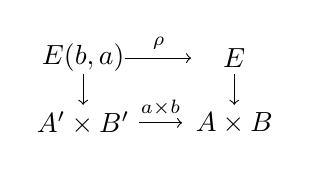
\begin{tikzpicture}[x=1.3em,y=1.3em]
  \node at (0,1.8) {$E(b,a)$};
  \node at (4.2,1.8) {$E$};
  \node at (0,0) {$A'\times B'$};
  \node at (4.2,0) {$A\times B$};
  \draw[->] (1.15,1.8) -- (3.0,1.8);
  \node at (2.1,2.22) {$\scriptstyle\rho$};
  \draw[->] (0,1.35) -- (0,0.5);
  \draw[->] (4.2,1.35) -- (4.2,0.5);
  \draw[->] (1.55,0) -- (2.75,0);
  \node at (2.15,0.42) {$\scriptstyle a\times b$};
  \node at (0.65,1.3) {$\scriptstyle\lrcorner$};
\end{tikzpicture}
\end{rveq}
由命题 7.4.5，这个左侧的\trIsofibration{}定义一个从 $A'$ 到 $B'$ 的\trModule{}；%
而由定义 8.1.4，其顶部的水平\trFunctor{}表示一个占据所求方块的\trModule{}映射。%
由观察 8.1.5，$\mathcal{K}$ 中的单纯\trPullback{}诱导\trFunctorSpace{}之间的%
如下\trEquivalence\footnote{若诸拉回按严格意义定义，则拉回事实上诱导%
\trFunctorSpace{}之间的一个\trIsomorphism；但即使把 $E(b,a)$ 换成一支等价的%
\trModule，诸\trFunctorSpace{}仍相等价，这已足以在对象的\trIsomorphism{}类上%
诱导一个双射。}
\begin{equation*}
\Fun_{f\times g}(E_{1}\times_{A_{1}}\cdots\times_{A_{n-1}}E_{n},\,E(b,a))
\xrightarrow[\ \simeq\ ]{\ \rho\circ-\ }
\Fun_{af\times bg}(E_{1}\times_{A_{1}}\cdots\times_{A_{n-1}}E_{n},\,E)
\end{equation*}
它在对象的\trIsomorphism{}类上下降为一个双射。这就给出了如上左图所示之胞腔%
经由笛卡尔的限制胞腔 $\rho$ 的唯一分解。
\end{proof}

我们把模 $A'\xrightarrow{E(b,a)}B'$ 称为模 $A\xrightarrow{E}B$ 沿函子 $a$ 与
$b$ 的\textbf{限制}（restriction），因为拉回 \eqref{eq:restriction-pullback}%
类似于双模沿一对环同态的\trRestrictionOfScalars。

\begin{example}\label{exa:hom-restriction}
模 $C\xrightarrow{\HomA(f,g)}B$ 是把由箭头 $\oo$-范畴
$A\overset{p_{1}}{\twoheadleftarrow}A^{2}\overset{p_{0}}{\twoheadrightarrow}A$
所编码的模沿 $g\colon C\to A$ 与 $f\colon B\to A$ 作限制的结果。为使这一限制%
关系更加透明，当把箭头 $\oo$-范畴视为一个\trModule{}时，我们通常把它写作
$A\xrightarrow{\HomA}A$。
\begin{center}
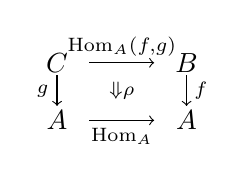
\begin{tikzpicture}[x=1.3em,y=1.3em]
  \node at (0,1.6) {$C$};
  \node at (3.6,1.6) {$B$};
  \node at (0,0) {$A$};
  \node at (3.6,0) {$A$};
  \draw[->] (0.9,1.6) -- (2.7,1.6);
  \node at (1.8,2.05) {$\scriptstyle\HomA(f,g)$};
  \draw[->] (0,1.25) -- (0,0.4);
  \node at (-0.4,0.82) {$\scriptstyle g$};
  \draw[->] (3.6,1.25) -- (3.6,0.4);
  \node at (4.0,0.82) {$\scriptstyle f$};
  \node at (1.8,0.82) {$\scriptstyle\Downarrow\rho$};
  \draw[->] (0.9,0) -- (2.7,0);
  \node at (1.8,-0.45) {$\scriptstyle\HomA$};
\end{tikzpicture}
\end{center}
由于 hom \trBifunctor{}的通行记法把逆变变元置于左侧、把协变变元置于右侧，我们在%
\cref{prop:restriction}中对限制采用了类似的记号约定。
\end{example}

\begin{proposition}[单位]\label{prop:units}
$\Mod(\mathcal{K})$ 中的任何对象 $A$ 都配备有一个零元\textbf{\trCocartesian%
\trCell}（cocartesian cell）
\begin{center}
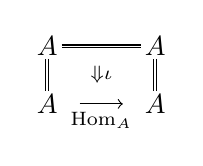
\begin{tikzpicture}[x=1.3em,y=1.3em]
  \node at (0,1.6) {$A$};
  \node at (3.0,1.6) {$A$};
  \node at (0,0) {$A$};
  \node at (3.0,0) {$A$};
  \draw[double,double distance=0.6pt] (0.4,1.6) -- (2.6,1.6);
  \draw[double,double distance=0.6pt] (0,1.25) -- (0,0.35);
  \draw[double,double distance=0.6pt] (3.0,1.25) -- (3.0,0.35);
  \node at (1.5,0.8) {$\scriptstyle\Downarrow\iota$};
  \draw[->] (0.9,0) -- (2.1,0);
  \node at (1.5,-0.45) {$\scriptstyle\HomA$};
\end{tikzpicture}
\end{center}
并由如下\trUniversalProperty{}刻画：$\Mod(\mathcal{K})$ 中任何水平源包含对象
$A$ 的胞腔都经由 $\iota$ 唯一地分解，如下所示：
\begin{center}
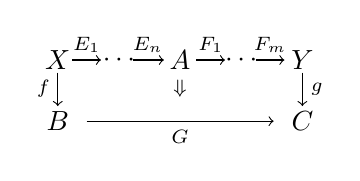
\begin{tikzpicture}[x=1.3em,y=1.3em]
  \node at (0,1.7) {$X$};
  \node at (1.7,1.7) {$\cdots$};
  \node at (3.4,1.7) {$A$};
  \node at (5.1,1.7) {$\cdots$};
  \node at (6.8,1.7) {$Y$};
  \draw[->] (0.4,1.7) -- (1.2,1.7);
  \node at (0.8,2.12) {$\scriptstyle E_{1}$};
  \draw[->] (2.1,1.7) -- (2.95,1.7);
  \node at (2.5,2.12) {$\scriptstyle E_{n}$};
  \draw[->] (3.85,1.7) -- (4.65,1.7);
  \node at (4.25,2.12) {$\scriptstyle F_{1}$};
  \draw[->] (5.5,1.7) -- (6.3,1.7);
  \node at (5.9,2.12) {$\scriptstyle F_{m}$};
  \draw[->] (0,1.35) -- (0,0.42);
  \node at (-0.4,0.9) {$\scriptstyle f$};
  \draw[->] (6.8,1.35) -- (6.8,0.42);
  \node at (7.2,0.9) {$\scriptstyle g$};
  \node at (3.4,0.9) {$\scriptstyle\Downarrow$};
  \node at (0,0) {$B$};
  \node at (6.8,0) {$C$};
  \draw[->] (0.8,0) -- (6.0,0);
  \node at (3.4,-0.45) {$\scriptstyle G$};
\end{tikzpicture}
\qquad $:=$
\end{center}
\begin{center}
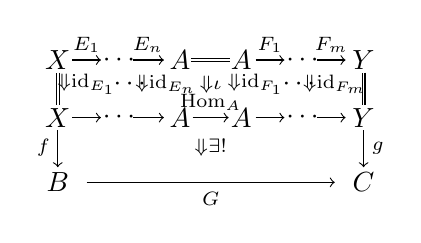
\begin{tikzpicture}[x=1.3em,y=1.3em]
  \node at (0,3.4) {$X$};
  \node at (1.7,3.4) {$\cdots$};
  \node at (3.4,3.4) {$A$};
  \node at (5.1,3.4) {$A$};
  \node at (6.8,3.4) {$\cdots$};
  \node at (8.5,3.4) {$Y$};
  \draw[->] (0.4,3.4) -- (1.2,3.4);
  \node at (0.8,3.82) {$\scriptstyle E_{1}$};
  \draw[->] (2.1,3.4) -- (2.95,3.4);
  \node at (2.5,3.82) {$\scriptstyle E_{n}$};
  \draw[double,double distance=0.6pt] (3.7,3.4) -- (4.8,3.4);
  \draw[->] (5.5,3.4) -- (6.3,3.4);
  \node at (5.9,3.82) {$\scriptstyle F_{1}$};
  \draw[->] (7.2,3.4) -- (8.0,3.4);
  \node at (7.6,3.82) {$\scriptstyle F_{m}$};
  \draw[double,double distance=0.6pt] (0,3.05) -- (0,2.15);
  \draw[double,double distance=0.6pt] (8.5,3.05) -- (8.5,2.15);
  \node at (0.8,2.72) {$\scriptstyle\Downarrow\mathrm{id}_{E_{1}}$};
  \node at (2.0,2.72) {$\cdots$};
  \node at (3.0,2.72) {$\scriptstyle\Downarrow\mathrm{id}_{E_{n}}$};
  \node at (4.25,2.72) {$\scriptstyle\Downarrow\iota$};
  \node at (5.5,2.72) {$\scriptstyle\Downarrow\mathrm{id}_{F_{1}}$};
  \node at (6.7,2.72) {$\cdots$};
  \node at (7.7,2.72) {$\scriptstyle\Downarrow\mathrm{id}_{F_{m}}$};
  \node at (0,1.8) {$X$};
  \node at (1.7,1.8) {$\cdots$};
  \node at (3.4,1.8) {$A$};
  \node at (5.1,1.8) {$A$};
  \node at (6.8,1.8) {$\cdots$};
  \node at (8.5,1.8) {$Y$};
  \draw[->] (0.4,1.8) -- (1.2,1.8);
  \draw[->] (2.1,1.8) -- (2.95,1.8);
  \draw[->] (3.75,1.8) -- (4.75,1.8);
  \node at (4.25,2.22) {$\scriptstyle\HomA$};
  \draw[->] (5.5,1.8) -- (6.3,1.8);
  \draw[->] (7.2,1.8) -- (8.0,1.8);
  \draw[->] (0,1.45) -- (0,0.42);
  \node at (-0.4,0.95) {$\scriptstyle f$};
  \draw[->] (8.5,1.45) -- (8.5,0.42);
  \node at (8.9,0.95) {$\scriptstyle g$};
  \node at (4.25,0.95) {$\scriptstyle\Downarrow\exists!$};
  \node at (0,0) {$B$};
  \node at (8.5,0) {$C$};
  \draw[->] (0.8,0) -- (7.7,0);
  \node at (4.25,-0.45) {$\scriptstyle G$};
\end{tikzpicture}
\end{center}
\end{proposition}

\begin{proof}
该零元胞腔由 $A$ 处的恒同 $1$-胞腔上的恒同 $2$-胞腔所诱导的\trSpan{}映射表示：
\begin{center}
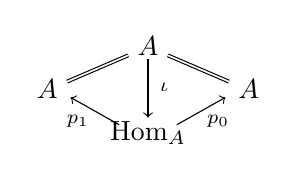
\begin{tikzpicture}[x=1.3em,y=1.3em]
  \node at (0,2.4) {$A$};
  \node at (-2.8,1.2) {$A$};
  \node at (2.8,1.2) {$A$};
  \node at (0,0) {$\HomA$};
  \draw[double,double distance=0.6pt] (-0.55,2.15) -- (-2.25,1.42);
  \draw[double,double distance=0.6pt] (0.55,2.15) -- (2.25,1.42);
  \draw[->] (0,2.05) -- (0,0.42);
  \node at (0.45,1.25) {$\scriptstyle\iota$};
  \draw[->] (-0.8,0.22) -- (-2.15,0.98);
  \node at (-1.95,0.32) {$\scriptstyle p_{1}$};
  \draw[->] (0.8,0.22) -- (2.15,0.98);
  \node at (1.95,0.32) {$\scriptstyle p_{0}$};
\end{tikzpicture}
\qquad $\mathrel{\leftrightsquigarrow}$ \qquad
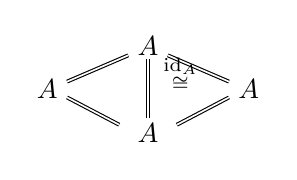
\begin{tikzpicture}[x=1.3em,y=1.3em]
  \node at (0,2.4) {$A$};
  \node at (-2.8,1.2) {$A$};
  \node at (2.8,1.2) {$A$};
  \node at (0,0) {$A$};
  \draw[double,double distance=0.6pt] (-0.55,2.15) -- (-2.25,1.42);
  \draw[double,double distance=0.6pt] (0.55,2.15) -- (2.25,1.42);
  \draw[double,double distance=0.6pt] (-2.25,0.98) -- (-0.8,0.22);
  \draw[double,double distance=0.6pt] (2.25,0.98) -- (0.8,0.22);
  \draw[double,double distance=0.6pt] (0,2.05) -- (0,0.42);
  \node at (0.9,1.85) {$\scriptstyle\mathrm{id}_{A}$};
  \node at (0.9,1.35) {$\scriptstyle\cong$};
\end{tikzpicture}
\end{center}
在别处，这个\trFunctor{}记作
$\ulcorner\mathrm{id}_{A}\urcorner\colon A\to A^{2}$；回忆%
\cref{exa:hom-restriction}：我们把箭头 $\oo$-范畴构造所编码的模写作
$A\xrightarrow{\HomA}A$，正是为了帮助我们识别它的诸限制。

在序列 $E_{i}$ 与 $F_{j}$ 皆为空的情形，由定理 7.4.8 给出的模的\trYonedaLemma{}%
的单侧版本告诉我们：沿这一映射的限制诱导\trFunctorSpace{}的一个\trEquivalence
\begin{equation*}
\Fun_{A\times A}(\HomA,G(g,f))
\Rightarrow
\Fun_{A\times A}(A,G(g,f)).
\end{equation*}
取对象的\trIsomorphism{}类即得该陈述中的双射。

在序列之一或两者皆非空的情形，我们可以作出把它们水平复合而成的%
\trTwoSidedFibration{} $X\xleftarrow{q}E\xrightarrow{p}A$ 与
$A\xleftarrow{s}F\xrightarrow{r}Y$，然后对如下可复合三元组作出水平复合
$E\times_{A}\HomA$ 或水平复合 $\HomA\times_{A}F$：
\begin{center}
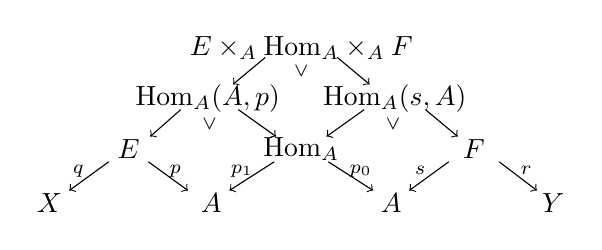
\begin{tikzpicture}[x=1.3em,y=1.3em]
  \node at (2.6,4.3) {$E\times_{A}\HomA\times_{A}F$};
  \node at (0,2.9) {$\HomA(A,p)$};
  \node at (5.2,2.9) {$\HomA(s,A)$};
  \node at (-2.2,1.5) {$E$};
  \node at (2.6,1.5) {$\HomA$};
  \node at (7.4,1.5) {$F$};
  \node at (-4.4,0) {$X$};
  \node at (0.1,0) {$A$};
  \node at (5.1,0) {$A$};
  \node at (9.6,0) {$Y$};
  \draw[->] (1.6,4.05) -- (0.7,3.3);
  \draw[->] (3.6,4.05) -- (4.5,3.3);
  \node at (2.6,3.68) {$\scriptstyle\vee$};
  \draw[->] (-0.75,2.6) -- (-1.6,1.85);
  \draw[->] (0.85,2.6) -- (1.9,1.85);
  \node at (0.05,2.2) {$\scriptstyle\vee$};
  \draw[->] (4.35,2.6) -- (3.3,1.85);
  \draw[->] (6.05,2.6) -- (6.95,1.85);
  \node at (5.15,2.2) {$\scriptstyle\vee$};
  \draw[->] (-2.75,1.15) -- (-3.85,0.35);
  \node at (-3.6,0.9) {$\scriptstyle q$};
  \draw[->] (-1.65,1.15) -- (-0.55,0.35);
  \node at (-0.9,0.9) {$\scriptstyle p$};
  \draw[->] (1.85,1.15) -- (0.6,0.35);
  \node at (0.95,0.9) {$\scriptstyle p_{1}$};
  \draw[->] (3.35,1.15) -- (4.6,0.35);
  \node at (4.25,0.9) {$\scriptstyle p_{0}$};
  \draw[->] (6.7,1.15) -- (5.6,0.35);
  \node at (5.9,0.9) {$\scriptstyle s$};
  \draw[->] (8.1,1.15) -- (9.15,0.35);
  \node at (8.85,0.9) {$\scriptstyle r$};
\end{tikzpicture}
\end{center}
左边那一对\trModule{}的水平复合是\trTwoSidedFibration{}
$(qp_{1},p_{0})\colon\HomA(A,p)\twoheadrightarrow X\times A$，而右边那一对的%
复合是\trTwoSidedFibration{}
$(p_{1},rp_{0})\colon\HomA(s,A)\twoheadrightarrow A\times Y$。由定理 7.1.4，%
这些\trTwoSidedFibration{}给出如下\trFiberedAdjunction：
\begin{center}
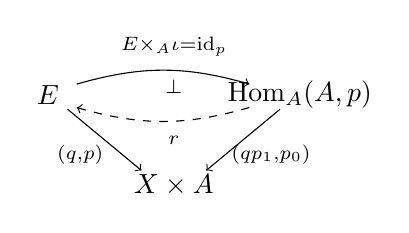
\begin{tikzpicture}[x=1.3em,y=1.3em]
  \node at (0,1.4) {$E$};
  \node at (7.0,1.4) {$\HomA(A,p)$};
  \node at (3.5,-1.1) {$X\times A$};
  \draw[->] (0.8,1.7) to[bend left=16] (5.6,1.7);
  \node at (3.5,2.75) {$\scriptstyle E\times_{A}\iota=\ulcorner\mathrm{id}_{p}\urcorner$};
  \node at (3.5,1.62) {$\scriptstyle\perp$};
  \draw[->,dashed] (5.6,1.05) to[bend left=16] (0.8,1.05);
  \node at (3.5,0.15) {$\scriptstyle r$};
  \draw[->] (0.55,1.0) -- (2.6,-0.7);
  \node at (0.9,-0.25) {$\scriptstyle(q,p)$};
  \draw[->] (6.45,1.0) -- (4.4,-0.7);
  \node at (6.2,-0.25) {$\scriptstyle(qp_{1},p_{0})$};
\end{tikzpicture}
\qquad
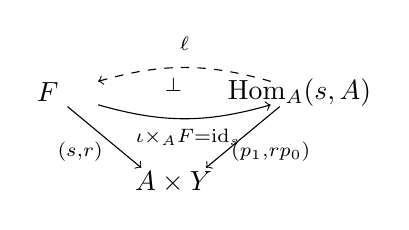
\begin{tikzpicture}[x=1.3em,y=1.3em]
  \node at (0,1.4) {$F$};
  \node at (7.0,1.4) {$\HomA(s,A)$};
  \node at (3.5,-1.1) {$A\times Y$};
  \draw[->,dashed] (6.2,1.7) to[bend right=16] (1.4,1.7);
  \node at (3.8,2.75) {$\scriptstyle\ell$};
  \node at (3.5,1.62) {$\scriptstyle\perp$};
  \draw[->] (1.4,1.05) to[bend right=16] (6.2,1.05);
  \node at (3.9,0.15) {$\scriptstyle\iota\times_{A}F=\ulcorner\mathrm{id}_{s}\urcorner$};
  \draw[->] (0.55,1.0) -- (2.6,-0.7);
  \node at (0.9,-0.25) {$\scriptstyle(s,r)$};
  \draw[->] (6.45,1.0) -- (4.4,-0.7);
  \node at (6.2,-0.25) {$\scriptstyle(p_{1},rp_{0})$};
\end{tikzpicture}
\end{center}

经直接观察，实线箭头的两根伴随 $\ulcorner\mathrm{id}_{p}\urcorner$ 与
$\ulcorner\mathrm{id}_{s}\urcorner$ 可以通过拉回映射 $\iota\colon A\to\HomA$ 而%
构造。

我们只需要其中一个伴随，故不失一般性地取前者。这一\trFiberedAdjunction{}沿 $s$ 拉回、沿 $r$
前推，定义出\trTwoSidedFibration{}之间的如下\trFiberedAdjunction
\begin{center}
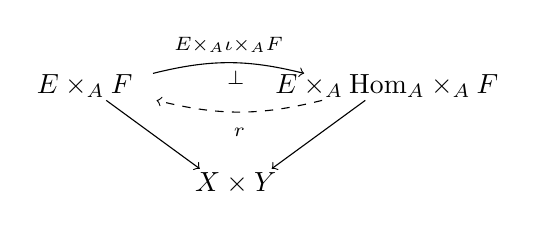
\begin{tikzpicture}[x=1.3em,y=1.3em]
  \node at (0,1.5) {$E\times_{A}F$};
  \node at (8.4,1.5) {$E\times_{A}\HomA\times_{A}F$};
  \node at (4.2,-1.2) {$X\times Y$};
  \draw[->] (1.9,1.85) to[bend left=14] node[above,pos=0.5]{$\scriptstyle E\times_{A}\iota\times_{A}F$} (6.1,1.85);
  \node at (4.2,1.72) {$\scriptstyle\perp$};
  \draw[->,dashed] (6.6,1.1) to[bend left=14] (2.0,1.1);
  \node at (4.3,0.2) {$\scriptstyle r$};
  \draw[->] (0.6,1.1) -- (3.2,-0.8);
  \draw[->] (7.8,1.1) -- (5.2,-0.8);
\end{tikzpicture}
\end{center}
当映入 $\mathcal{K}_{/X\times Y}$ 中的\trDiscrete{}对象 $G(g,f)$ 时，这一伴随%
成为一个\trAdjointEquivalence{}。特别地，沿 $\iota$ 的限制诱导\trKanComplex{}之间%
的一个\trEquivalence
\begin{equation*}
\Fun_{X\times Y}(E\times_{A}\HomA\times_{A}F,\,G(g,f))
\xrightarrow[\ \simeq\ ]{\ -\circ(E\times_{A}\iota\times_{A}F)\ }
\Fun_{X\times Y}(E\times_{A}F,\,G(g,f)),
\end{equation*}
而再一次取对象的\trIsomorphism{}类即给出该陈述中的双射。
\end{proof}

\cref{prop:restriction}与\cref{prop:units}蕴含：模的\trVirtualDoubleCategory{}是 Cruttwell 与
Shulman（\cite{bib32}，第 7 节）所引入意义下的一个\emph{\trVirtualEquipment}。

\begin{definition}\label{def:virtual-equipment}
一个\textbf{\trVirtualEquipment}是一个满足如下条件的\trVirtualDoubleCategory{}：
\begin{enumerate}[label=(\roman*)]
\item 对任何水平箭头 $A\xrightarrow{E}B$ 与任何一对竖直箭头
$a\colon A'\to A$ 和 $b\colon B'\to B$，都存在一个水平箭头
$A'\xrightarrow{E(b,a)}B'$\footnote{原书印作「$B'\xrightarrow{E(b,a)}A'$」。
按\cref{prop:restriction}，限制 $E(b,a)$ 是从 $A'$ 到 $B'$ 的\trModule{}（该
命题图示顶行即 $A'\xrightarrow{E(b,a)}B'$），疑原书方向笔误，此处径改。
——译者注}与一个满足\cref{prop:restriction}之%
\trUniversalProperty{}的一元\trCartesian\trCell{} $\rho$。
\item 每个对象 $A$ 都具备一个\textbf{单位}（unit）水平箭头
$A\xrightarrow{\HomA}A$，并配备有一个满足\cref{prop:units}之%
\trUniversalProperty{}的零元\trCocartesian\trCell{} $\iota$。
\end{enumerate}
\end{definition}

这样，\cref{prop:restriction}与\cref{prop:units}结合起来便证明：

\begin{theorem}\label{thm:modules-virtual-equipment}
\trInfinityCosmos{} $\mathcal{K}$ 中的模的\trVirtualDoubleCategory $\Mod(\mathcal{K})$ 是一个%
\trVirtualEquipment{}。
\end{theorem}

凭抽象废话，\cref{thm:modules-virtual-equipment} 所确立的%
\cref{def:virtual-equipment}(i) 与 (ii) 这两条相对简单的公理，就建立起一套%
稳健的「模的演算」。为了让读者熟悉这一鲜为人知的范畴结构，并为第 9 章中
$\oo$-范畴之形式范畴论的证明提速，我们将本章的剩余部分用于证明一大批实际上%
可以从这一公理化形式地推出的结果：即引理 8.3.10 与引理 8.3.15、命题 8.4.1、%
定理 8.4.4、推论 8.4.6、命题 8.4.7、推论 8.4.8、推论 8.4.9，以及命题 8.4.11
关于模的虚拟装备中一元胞腔的双射\footnote{一个细微的差别在于：我们在此观察到，%
这些陈述中许多所引用的复合都是「强」的——这一概念在一般的虚拟装备中并无%
意义。}。另有一个形式结果留给读者，见练习 8.4.v。

\begin{notation}\label{not:virtual-equipment-notation}
下面的记号约定使某些虚拟装备图式变得精简。
\begin{itemize}
\item 我们采用如下约定：竖直边界皆为恒同、且水平源与水平目标相一致的未标注%
一元胞腔是恒同胞腔。
\begin{center}
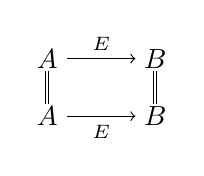
\begin{tikzpicture}[x=1.3em,y=1.3em]
  \node at (0,1.6) {$A$};
  \node at (3.0,1.6) {$B$};
  \node at (0,0) {$A$};
  \node at (3.0,0) {$B$};
  \draw[->] (0.55,1.6) -- (2.45,1.6);
  \node at (1.5,2.02) {$\scriptstyle E$};
  \draw[double,double distance=0.6pt] (0,1.25) -- (0,0.35);
  \draw[double,double distance=0.6pt] (3.0,1.25) -- (3.0,0.35);
  \draw[->] (0.55,0) -- (2.45,0);
  \node at (1.5,-0.45) {$\scriptstyle E$};
\end{tikzpicture}
\qquad $:=$ \qquad
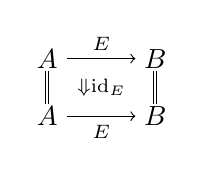
\begin{tikzpicture}[x=1.3em,y=1.3em]
  \node at (0,1.6) {$A$};
  \node at (3.0,1.6) {$B$};
  \node at (0,0) {$A$};
  \node at (3.0,0) {$B$};
  \draw[->] (0.55,1.6) -- (2.45,1.6);
  \node at (1.5,2.02) {$\scriptstyle E$};
  \draw[double,double distance=0.6pt] (0,1.25) -- (0,0.35);
  \draw[double,double distance=0.6pt] (3.0,1.25) -- (3.0,0.35);
  \node at (1.5,0.8) {$\scriptstyle\Downarrow\mathrm{id}_{E}$};
  \draw[->] (0.55,0) -- (2.45,0);
  \node at (1.5,-0.45) {$\scriptstyle E$};
\end{tikzpicture}
\end{center}
\item 竖直边界函子为恒同、从而其源\trSpan{}与目标\trSpan{}都居于同一对
$\oo$-范畴之间的胞腔
\begin{center}
$\mu\colon E_{1}\divideontimes\cdots\divideontimes E_{n}\Rightarrow E$
\qquad $:=$ \qquad
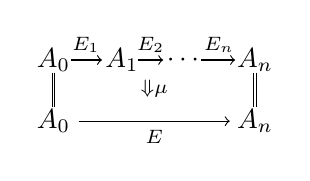
\begin{tikzpicture}[x=1.3em,y=1.3em]
  \node at (0,1.7) {$A_{0}$};
  \node at (1.9,1.7) {$A_{1}$};
  \node at (3.6,1.7) {$\cdots$};
  \node at (5.6,1.7) {$A_{n}$};
  \draw[->] (0.5,1.7) -- (1.35,1.7);
  \node at (0.9,2.12) {$\scriptstyle E_{1}$};
  \draw[->] (2.35,1.7) -- (3.05,1.7);
  \node at (2.7,2.12) {$\scriptstyle E_{2}$};
  \draw[->] (4.1,1.7) -- (5.05,1.7);
  \node at (4.6,2.12) {$\scriptstyle E_{n}$};
  \draw[double,double distance=0.6pt] (0,1.35) -- (0,0.4);
  \draw[double,double distance=0.6pt] (5.6,1.35) -- (5.6,0.4);
  \node at (2.8,0.9) {$\scriptstyle\Downarrow\mu$};
  \node at (0,0) {$A_{0}$};
  \node at (5.6,0) {$A_{n}$};
  \draw[->] (0.7,0) -- (4.9,0);
  \node at (2.8,-0.45) {$\scriptstyle E$};
\end{tikzpicture}
\end{center}
可以用记号 $\mu\colon E_{1}\divideontimes\cdots\divideontimes E_{n}\Rightarrow E$ 排入行内；%
这一表述隐含地断言，定义域中出现的诸\trModule{}定义一个相容序列，其中符号%
「$\divideontimes$」意在暗示 (8.1.9) 中作为水平定义域出现的那个\trPullback{}，而非%
一个\trProduct{}。在模的虚拟装备中，形如
$\mu\colon E_{1}\divideontimes\cdots\divideontimes E_{n}\Rightarrow E$ 的胞腔对应于定义
8.1.1 所引入意义下的\emph{纤维化映射}（fibered maps）。
\item 给定从 $A_{0}$ 到 $A_{n}$ 的一个相容\trModule{}序列
$E_{1}\divideontimes\cdots\divideontimes E_{n}$，我们记
$A_{0}\mathrel{\overset{\vec{E}}{\leftrightsquigarrow}}A_{n}$ 表示复合而成的%
\trTwoSidedFibration{}，并类似地把以该序列为源的一个 $n$ 元\trModule{}映射
(8.1.9) 缩写为如下左图：
\begin{center}
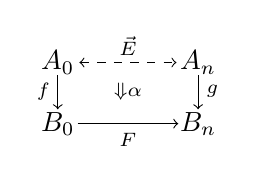
\begin{tikzpicture}[x=1.3em,y=1.3em]
  \node at (0,1.7) {$A_{0}$};
  \node at (3.9,1.7) {$A_{n}$};
  \draw[<->,dashed] (0.6,1.7) -- (3.3,1.7);
  \node at (1.95,2.15) {$\scriptstyle\vec{E}$};
  \draw[->] (0,1.35) -- (0,0.4);
  \node at (-0.4,0.9) {$\scriptstyle f$};
  \draw[->] (3.9,1.35) -- (3.9,0.4);
  \node at (4.3,0.9) {$\scriptstyle g$};
  \node at (1.95,0.9) {$\scriptstyle\Downarrow\alpha$};
  \node at (0,0) {$B_{0}$};
  \node at (3.9,0) {$B_{n}$};
  \draw[->] (0.55,0) -- (3.35,0);
  \node at (1.95,-0.45) {$\scriptstyle F$};
\end{tikzpicture}
\qquad $:=$ \qquad
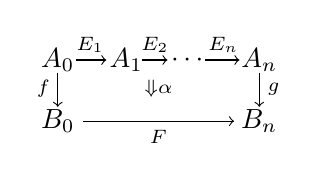
\begin{tikzpicture}[x=1.3em,y=1.3em]
  \node at (0,1.7) {$A_{0}$};
  \node at (1.9,1.7) {$A_{1}$};
  \node at (3.6,1.7) {$\cdots$};
  \node at (5.6,1.7) {$A_{n}$};
  \draw[->] (0.5,1.7) -- (1.35,1.7);
  \node at (0.9,2.12) {$\scriptstyle E_{1}$};
  \draw[->] (2.35,1.7) -- (3.05,1.7);
  \node at (2.7,2.12) {$\scriptstyle E_{2}$};
  \draw[->] (4.1,1.7) -- (5.05,1.7);
  \node at (4.6,2.12) {$\scriptstyle E_{n}$};
  \draw[->] (0,1.35) -- (0,0.4);
  \node at (-0.4,0.9) {$\scriptstyle f$};
  \draw[->] (5.6,1.35) -- (5.6,0.4);
  \node at (6.0,0.9) {$\scriptstyle g$};
  \node at (2.8,0.9) {$\scriptstyle\Downarrow\alpha$};
  \node at (0,0) {$B_{0}$};
  \node at (5.6,0) {$B_{n}$};
  \draw[->] (0.7,0) -- (4.9,0);
  \node at (2.8,-0.45) {$\scriptstyle F$};
\end{tikzpicture}
\end{center}
\end{itemize}
\end{notation}
   %
\providecommand{\Mod}{\mathbb{M}od}
\providecommand{\Fun}{\operatorname{Fun}}
\providecommand{\HomA}{\mathrm{Hom}_{A}}
\providecommand{\HomB}{\mathrm{Hom}_{B}}
\providecommand{\HomC}{\mathrm{Hom}_{C}}
\providecommand{\Homf}{\mathrm{Hom}_{f}}
\providecommand{\Homg}{\mathrm{Hom}_{g}}

\subsection*{练习}

\begin{exercise}\label{ex:restriction-hom-along-functors}
设有\trFunctor{}图表
$E\xrightarrow{k}C\xrightarrow{g}A\xleftarrow{f}B\xleftarrow{h}D$，试计算模
$C\xrightarrow{\HomA(f,g)}B$ 沿\trFunctor{} $k$ 与 $h$ 作限制的结果。
\end{exercise}

\begin{exercise}\label{ex:unital-rings-bimodules-equipment}
证明：幺环、环同态、双模与双模映射也定义一个\trVirtualEquipment。
\end{exercise}

\begin{exercise}\label{ex:two-sided-isofibrations-virtual-equipment}
证明：双侧等价纤维化的\trVirtualDoubleCategory{}连同注 8.1.13 的单位%
\trCell{}一起构成一个\trVirtualEquipment。
\end{exercise}

\section{模的复合}\label{sec:composition-of-modules}

在一个\trVirtualEquipment{}中，并不假定任意一对水平箭头
$A\xrightarrow{E}B$ 与 $B\xrightarrow{F}C$ 都容许一个复合，但存在一套机制，
当某个特定的水平复合 $A\xrightarrow{G}C$ 恰好存在时能将其识别出来。当 $G$ 是
$E$ 与 $F$ 的水平复合时，我们记 $E\otimes F\simeq G$ 或
$\mu\colon E\otimes F\simeq G$，以强化双模类比所提供的直觉。

在模的\trVirtualEquipment{}中，对于模的「水平复合」我们可以赋予两种可能的含
义。第一种含义下，一个复合关系 $\mu\colon E\otimes F\simeq G$ 由一支纤维化
模映射 $\mu\colon E\times_{B}F\xrightarrow{}G$ 见证，后者以与命题 8.2.4 所述%
\trUniversalProperty{}相类比的方式定义一个\trCocartesian\trCell{}（见%
\cref{def:composite}）。这一复合定义可以在任何\trVirtualDoubleCategory{}中给
出，并且在任何\trVirtualEquipment{}——例如模的\trVirtualEquipment——中都表
现良好。可复合模的 $n$ 元序列的复合可以类似地定义。

在模的\trVirtualEquipment{}中，我们形式地定义的所有复合都满足一个更强的、在%
\trInfinityCosmos{}层面表述的\trUniversalProperty。回忆：模
$A\xrightarrow{E}B$、$B\xrightarrow{F}C$ 与 $A\xrightarrow{G}C$ 之间的一支纤
维化映射 $\mu\colon E\times_{B}F\xrightarrow{}G$ 对应于 $A\times C$ 之上的一个%
\trSpan{}映射 $\ulcorner\mu\urcorner\colon E\times_{B}F\to G$ 的纤维化同构
类。说 $\mu$ 在\cref{def:strong-composite}中见证一个\emph{强复合}（strong
composite），其部分含义是要求：它的表示函子对每个模 $A\xrightarrow{H}C$ 都诱
导 Kan 复形的如下\trEquivalence
$-\circ\ulcorner\mu\urcorner\colon\Fun_{A\times C}(G,H)\sim\Fun_{A\times C}(E\times_{B}F,H)$。一旦如此，模 $G$

便可理解为双侧等价纤维化 $E\times_{B}F$ 向诸模之子范畴中的「反射」；然而请注
意，$G$ 与 $E\times_{B}F$ 在 $A\times C$ 之上未必\trEquivalence。定理 7.3.2
的一个特例——它将以\cref{prop:composite-of-legs}的面貌再次出现——就是强复合
的一个实例。

正如这一术语所暗示的，强复合必为复合。既然「作为复合」这一较弱的%
\trUniversalProperty{}在纤维化\trEquivalence{}的意义下刻画了复合模，那么当我
们身处一个保证强复合存在的\trInfinityCosmos{}中时，我们现在引入的 2-范畴式%
\trUniversalProperty{}便足以把它们检测出来。\footnote{这类似于命题 5.2.11 中
所考虑的「定义弱 $p$-笛卡尔变换的\trUniversalProperty{}」与「定义 $p$-笛卡尔
变换的\trUniversalProperty{}」二者之间的关系。}

\begin{definition}\label{def:composite}
模的一个相容序列
\begin{equation*}
A\xrightarrow{E_{1}}A_{1},\ A_{1}\xrightarrow{E_{2}}A_{2},\ \ldots,\
A_{n-1}\xrightarrow{E_{n}}B
\end{equation*}
容许一个\textbf{复合}（composite），如果存在一个模 $A\xrightarrow{E}B$ 与一
个\trCocartesian\trCell
\begin{equation*}
\mu\colon E_{1}\divideontimes\cdots\divideontimes E_{n}\Rightarrow E
\end{equation*}
它由如下\trUniversalProperty{}刻画：任何形如下图的胞腔
\begin{center}
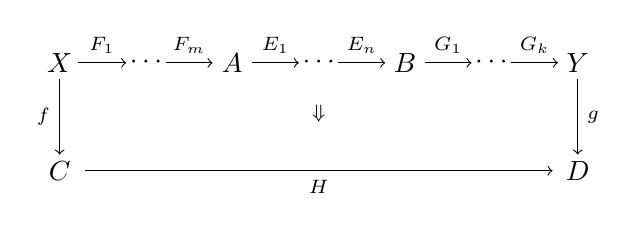
\begin{tikzpicture}[x=1.3em,y=1.3em]
  \node at (0,1.5) {$X$};
  \node at (2.4,1.5) {$\cdots$};
  \node at (4.8,1.5) {$A$};
  \node at (7.2,1.5) {$\cdots$};
  \node at (9.6,1.5) {$B$};
  \node at (12.0,1.5){$\cdots$};
  \node at (14.4,1.5){$Y$};
  \draw[->] (0.5,1.5) -- node[above]{$\scriptstyle F_{1}$} (1.85,1.5);
  \draw[->] (2.95,1.5) -- node[above]{$\scriptstyle F_{m}$} (4.25,1.5);
  \draw[->] (5.35,1.5) -- node[above]{$\scriptstyle E_{1}$} (6.65,1.5);
  \draw[->] (7.75,1.5) -- node[above]{$\scriptstyle E_{n}$} (9.05,1.5);
  \draw[->] (10.15,1.5) -- node[above]{$\scriptstyle G_{1}$} (11.45,1.5);
  \draw[->] (12.55,1.5) -- node[above]{$\scriptstyle G_{k}$} (13.85,1.5);
  \node at (7.2,0.1) {$\scriptstyle\Downarrow$};
  \node at (0,-1.5) {$C$};
  \node at (14.4,-1.5){$D$};
  \draw[->] (0,1.05) -- node[left]{$\scriptstyle f$} (0,-1.05);
  \draw[->] (14.4,1.05) -- node[right]{$\scriptstyle g$} (14.4,-1.05);
  \draw[->] (0.7,-1.5) -- node[below]{$\scriptstyle H$} (13.7,-1.5);
\end{tikzpicture}
\end{center}
都唯一地穿过 $\mu$ 分解，如下所示：
\begin{center}
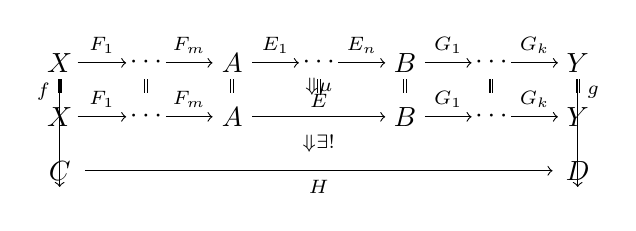
\begin{tikzpicture}[x=1.3em,y=1.3em]
  \node at (0,3.0) {$X$};
  \node at (2.4,3.0) {$\cdots$};
  \node at (4.8,3.0) {$A$};
  \node at (7.2,3.0) {$\cdots$};
  \node at (9.6,3.0) {$B$};
  \node at (12.0,3.0){$\cdots$};
  \node at (14.4,3.0){$Y$};
  \draw[->] (0.5,3.0) -- node[above]{$\scriptstyle F_{1}$} (1.85,3.0);
  \draw[->] (2.95,3.0) -- node[above]{$\scriptstyle F_{m}$} (4.25,3.0);
  \draw[->] (5.35,3.0) -- node[above]{$\scriptstyle E_{1}$} (6.65,3.0);
  \draw[->] (7.75,3.0) -- node[above]{$\scriptstyle E_{n}$} (9.05,3.0);
  \draw[->] (10.15,3.0) -- node[above]{$\scriptstyle G_{1}$} (11.45,3.0);
  \draw[->] (12.55,3.0) -- node[above]{$\scriptstyle G_{k}$} (13.85,3.0);
  \draw[double] (0,2.55) -- (0,2.15);
  \draw[double] (2.4,2.55) -- (2.4,2.15);
  \draw[double] (4.8,2.55) -- (4.8,2.15);
  \draw[double] (7.2,2.55) -- (7.2,2.15);
  \draw[double] (9.6,2.55) -- (9.6,2.15);
  \draw[double] (12.0,2.55) -- (12.0,2.15);
  \draw[double] (14.4,2.55) -- (14.4,2.15);
  \node at (7.2,2.35) {$\scriptstyle\Downarrow\mu$};
  \node at (0,1.5) {$X$};
  \node at (2.4,1.5) {$\cdots$};
  \node at (4.8,1.5) {$A$};
  \node at (9.6,1.5) {$B$};
  \node at (12.0,1.5){$\cdots$};
  \node at (14.4,1.5){$Y$};
  \draw[->] (0.5,1.5) -- node[above]{$\scriptstyle F_{1}$} (1.85,1.5);
  \draw[->] (2.95,1.5) -- node[above]{$\scriptstyle F_{m}$} (4.25,1.5);
  \draw[->] (5.35,1.5) -- node[above]{$\scriptstyle E$} (9.05,1.5);
  \draw[->] (10.15,1.5) -- node[above]{$\scriptstyle G_{1}$} (11.45,1.5);
  \draw[->] (12.55,1.5) -- node[above]{$\scriptstyle G_{k}$} (13.85,1.5);
  \node at (7.2,0.75) {$\scriptstyle\Downarrow\exists!$};
  \node at (0,0) {$C$};
  \node at (14.4,0){$D$};
  \draw[->] (0.7,0) -- node[below]{$\scriptstyle H$} (13.7,0);
  \draw[->] (0,2.55) -- node[left,pos=0.12]{$\scriptstyle f$} (0,-0.45);
  \draw[->] (14.4,2.55) -- node[right,pos=0.12]{$\scriptstyle g$} (14.4,-0.45);
\end{tikzpicture}
\end{center}
\end{definition}

我们已经见过这一定义的一个实例。命题 8.2.4 证明：在模的\trVirtualEquipment{}%
中，诸单位定义零元复合 $\iota\colon\varnothing\Rightarrow \HomA$。

\begin{observation}[复合的唯一性]\label{obs:uniqueness-of-composites}
直接由这一\trUniversalProperty{}可知：在模的\trVirtualEquipment{}中，复合在
竖直\trIsomorphism{}的意义下唯一。回忆引理 8.1.17：平行的诸模在%
\trVirtualEquipment{}中竖直同构，当且仅当它们在通常的纤维化意义下%
\trEquivalence。
\end{observation}

一个复合 $\mu\colon E_{1}\divideontimes\cdots\divideontimes E_{n}\Rightarrow E$ 可以用来缩
减胞腔的定义域：凡出现从 $A$ 到 $B$ 的相容序列
$E_{1}\divideontimes\cdots\divideontimes E_{n}$ 之处，都代之以单个模 $E$。特别是在二元复合
的情形，我们记 $E_{1}\otimes E_{2}$ 表示模 $E_{1}$ 与 $E_{2}$ 的复合——它作
为\trCocartesian\trCell{} $E_{1}\divideontimes E_{2}\Rightarrow E_{1}\otimes E_{2}$
的余定义域出现。请注意，\cref{def:composite}的\trUniversalProperty{}所要求的
多于单纯要求 $\mu\colon E_{1}\divideontimes E_{2}\Rightarrow E_{1}\otimes E_{2}$ 在
源为 $E_{1}\divideontimes E_{2}$ 的诸二元胞腔之中具有普遍性之条件。正如 Hermida 所观察
到的，那较弱的\trUniversalProperty{}不足以证明模的张量积是结合的（见%
\cite{bib53} 的 §8.1 以及\cref{ex:virtual-double-composites}）。相比之下，%
\cref{def:composite}的\trUniversalProperty{}允许我们对三元及更高的复合使用诸
如 $E_{1}\otimes E_{2}\otimes E_{3}$ 的、不带括号的表达式，因为复合在如下意
义上是「结合的」：

\begin{lemma}\label{lem:composite-associativity}
设诸\trCell{} $\mu_{i}\colon E_{i1}\divideontimes\cdots\divideontimes E_{ik_{i}}\Rightarrow E_{i}$（$i=1,\ldots,n$）展示复合。

\begin{enumerate}[label=(\roman*)]
\item 若 $\mu\colon E_{1}\divideontimes\cdots\divideontimes E_{n}\Rightarrow E$ 展示一个复
合，则复合\trCell
\begin{equation*}
E_{11}\divideontimes\cdots\divideontimes E_{nk_{n}}
\xrightarrow{\ \mu_{1}\times\cdots\times\mu_{n}\ }
E_{1}\divideontimes\cdots\divideontimes E_{n}
\xrightarrow{\ \mu\ }
E
\end{equation*}
将 $E$ 展示为序列 $E_{11}\divideontimes\cdots\divideontimes E_{nk_{n}}$ 的一个复合。
\item 若该复合\trCell
\begin{equation*}
E_{11}\divideontimes\cdots\divideontimes E_{nk_{n}}
\xrightarrow{\ \mu_{1}\times\cdots\times\mu_{n}\ }
E_{1}\divideontimes\cdots\divideontimes E_{n}
\xrightarrow{\ \mu\ }
E
\end{equation*}
将 $E$ 展示为序列 $E_{11}\divideontimes\cdots\divideontimes E_{nk_{n}}$ 的一个复合，则
$\mu\colon E_{1}\divideontimes\cdots\divideontimes E_{n}\Rightarrow E$ 将 $E$ 展示为序列
$E_{1}\divideontimes\cdots\divideontimes E_{n}$ 的一个复合。
\end{enumerate}
\end{lemma}

\begin{proof}
对 (i)：所需的双射分解为由映射 $\mu_{1},\ldots,\mu_{n}$ 与 $\mu$ 诱导的
$n+1$ 个双射的复合。对 (ii)：由 $\mu$ 诱导的所需双射与由映射
$\mu_{1},\ldots,\mu_{n}$ 所提供的诸双射复合成一个双射，从而其本身也是一个双
射。
\end{proof}

\begin{remark}\label{rem:fibered-cells-suffice}
由于命题 8.2.1 所确立的限制之\trUniversalProperty，要证明一个\trCell{}
$\mu\colon E_{1}\divideontimes\cdots\divideontimes E_{n}\Rightarrow E$ 在某个%
\trVirtualEquipment{}中展示复合，只需在诸竖直\trFunctor{}皆为恒同的情形——
即所有\trCell{}皆为「\trFibered」之时——证明\cref{def:composite}的分解性质。
\end{remark}

\begin{definition}\label{def:strong-composite}
模的一个相容序列
\begin{equation*}
A\xrightarrow{E_{1}}A_{1},\ A_{1}\xrightarrow{E_{2}}A_{2},\ \ldots,\
A_{n-1}\xrightarrow{E_{n}}B
\end{equation*}
容许一个\textbf{强复合}，如果存在一个模 $A\xrightarrow{E}B$ 与一个%
\trFibered\trCell{} $\mu\colon E_{1}\divideontimes\cdots\divideontimes E_{n}\Rightarrow E$，
它由 $A\times B$ 之上的一个\trFunctor{}
$\ulcorner\mu\urcorner\colon E_{1}\divideontimes\cdots\divideontimes E_{n}\to E$ 表示，使
得对从 $X$ 到 $A$ 的所有相容模序列 $F_{1},\ldots,F_{m}$、从 $B$ 到 $Y$ 的所
有相容模序列 $G_{1},\ldots,G_{k}$ 以及所有模 $X\xrightarrow{H}Y$，这一%
\trFunctor{}都诱导 Kan 复形的如下\trEquivalence
\begin{equation*}
\Fun_{X\times Y}(\vec{F}\times_{A}E\times_{B}\vec{G},\,H)
\xrightarrow[\ \simeq\ ]{\,-\circ(\vec{F}\times_{A}\mu\times_{B}\vec{G})\,}
\Fun_{X\times Y}(\vec{F}\times_{A}E_{1}\times_{A_{1}}\cdots\times_{A_{n-1}}E_{n}\times_{B}\vec{G},\,H)
\end{equation*}
\end{definition}

\begin{lemma}[强复合皆为复合]\label{lem:strong-composites-are-composites}
若 $\mu\colon E_{1}\divideontimes\cdots\divideontimes E_{n}\Rightarrow E$ 是一个强复合，则
$\mu$ 将 $E$ 展示为复合 $E_{1}\otimes\cdots\otimes E_{n}$。
\end{lemma}

\begin{proof}
给定从 $X$ 到 $A$ 的一个相容模序列 $F_{1},\ldots,F_{m}$ 与从 $B$ 到 $Y$ 的
一个相容模序列 $G_{1},\ldots,G_{k}$，作出复合而成的双侧纤维化
$X\overset{q}{\twoheadleftarrow}\vec{F}\overset{p}{\twoheadrightarrow}A$ 与
$B\overset{s}{\twoheadleftarrow}\vec{G}\overset{r}{\twoheadrightarrow}Y$。由%
\cref{rem:fibered-cells-suffice}，只需对余定义域为模 $X\xrightarrow{H}Y$ 的那
些\trFibered{}映射检验复合\trCell{}的\trUniversalProperty。「$\mu$ 是强复合」
这一假设提供了 Kan 复形的\trEquivalence\footnote{原书此显示式右端
$\Fun$ 之下标印作 $A\times B$。按\cref{def:strong-composite}（其中两处下标
均为 $X\times Y$）及此处变元的边界（$H$ 为从 $X$ 到 $Y$ 的模），该下标应为
$X\times Y$，疑原书笔误，此处径改。——译者注}
\begin{equation*}
\Fun_{X\times Y}(\vec{F}\times_{A}E\times_{B}\vec{G},\,H)
\xrightarrow[\ \simeq\ ]{\,-\circ(\vec{F}\times_{A}\mu\times_{B}\vec{G})\,}
\Fun_{X\times Y}(\vec{F}\times_{A}E_{1}\times_{A_{1}}\cdots\times_{A_{n-1}}E_{n}\times_{B}\vec{G},\,H)
\end{equation*}
Kan 复形之间的一个\trEquivalence{}在道路连通分支上定义一个双射，而由观察
8.1.2，每个道路连通分支恰对应于诸\trFunctor{}的一个\trIsomorphism{}类。
\end{proof}

乍看之下，「强复合」的定义显得强得不合理。诸例将产生于命题 8.2.4 之证明所用
的同一结构，该证明展示了在模的\trVirtualEquipment{}中诸单位定义零元复合。

\begin{lemma}\label{lem:fibered-adjoint-strong-composite}
考虑模的\trVirtualEquipment{}中一个 $n$ 元模映射
$\mu\colon E_{1}\divideontimes\cdots\divideontimes E_{n}\Rightarrow E$，其余定义域为从 $A$
到 $B$ 的一个模。若任意一个表示它的\trSpan{}映射
\begin{center}
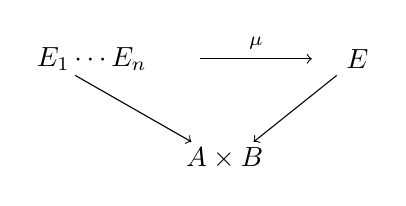
\begin{tikzpicture}[x=1.5em,y=1.5em]
  \node at (0,1.3) {$E_{1}\divideontimes\cdots\divideontimes E_{n}$};
  \node at (6.4,1.3) {$E$};
  \node at (3.2,-1.1) {$A\times B$};
  \draw[->] (2.6,1.3) -- node[above]{$\scriptstyle\ulcorner\mu\urcorner$} (5.3,1.3);
  \draw[->] (-0.4,0.9) -- (2.4,-0.7);
  \draw[->] (5.9,0.9) -- (3.9,-0.7);
\end{tikzpicture}
\end{center}
在 $A\times B$ 之上容许一个\trFiberedAdjunction，则 $\mu$ 将 $E$ 展示为强复合
$E_{1}\otimes\cdots\otimes E_{n}$。
\end{lemma}

\begin{proof}
为检验\cref{def:strong-composite}的\trUniversalProperty，考虑从 $X$ 到 $A$
的一个相容模序列 $F_{1},\ldots,F_{m}$ 与从 $B$ 到 $Y$ 的一个相容模序列
$G_{1},\ldots,G_{k}$，并作出水平复合而成的双侧纤维化
$X\overset{q}{\twoheadleftarrow}\vec{F}\overset{p}{\twoheadrightarrow}A$ 与
$B\overset{s}{\twoheadleftarrow}\vec{G}\overset{r}{\twoheadrightarrow}Y$。所
述的\trFiberedAdjunction{}沿 $p\times s\colon F\times G\to A\times B$ 拉回、沿
$q\times r\colon F\times G\to X\times Y$ 前推，得出一个\trFiberedAdjunction
\begin{center}
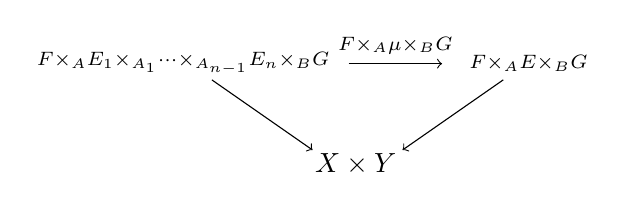
\begin{tikzpicture}[x=1.3em,y=1.3em]
  \node at (0,1.6)
    {$\scriptstyle F\times_{A}E_{1}\times_{A_{1}}\cdots\times_{A_{n-1}}E_{n}\times_{B}G$};
  \node at (9.6,1.6) {$\scriptstyle F\times_{A}E\times_{B}G$};
  \node at (4.8,-1.2) {$X\times Y$};
  \draw[->] (4.6,1.6) -- node[above]{$\scriptstyle F\times_{A}\ulcorner\mu\urcorner\times_{B}G$} (7.2,1.6);
  \draw[->] (0.8,1.15) -- (3.6,-0.8);
  \draw[->] (8.9,1.15) -- (6.1,-0.8);
\end{tikzpicture}
\end{center}
经由\cref{rem:fibered-cells-suffice}，只需对模 $X\xrightarrow{H}Y$ 检验复合
的\trUniversalProperty。由于模是\trDiscrete，施用 $\Fun_{X\times Y}(-,H)$
便将这一\trFiberedAdjunction{}变换为一个\trAdjointEquivalence
\begin{equation*}
\Fun_{X\times Y}(\vec{F}\times_{A}E\times_{B}\vec{G},\,H)
\xrightarrow[\ \simeq\ ]{\,-\circ(\vec{F}\times_{A}\ulcorner\mu\urcorner\times_{B}\vec{G})\,}
\Fun_{X\times Y}(\vec{F}\times_{A}E_{1}\times_{A_{1}}\cdots\times_{A_{n-1}}E_{n}\times_{B}\vec{G},\,H),
\end{equation*}
这就确立了刻画强复合的\trUniversalProperty。
\end{proof}

强复合满足一条与\cref{lem:composite-associativity}相类似的结合性质，其证明亦
类似：

\begin{lemma}\label{lem:strong-composite-associativity}
设诸\trCell{} $\mu_{i}\colon E_{i1}\divideontimes\cdots\divideontimes E_{ik_{i}}\Rightarrow E_{i}$（$i=1,\ldots,n$）展示强复合。

\begin{enumerate}[label=(\roman*)]
\item 若 $\mu\colon E_{1}\divideontimes\cdots\divideontimes E_{n}\Rightarrow E$ 展示一个强
复合，则复合\trCell
\begin{equation*}
E_{11}\divideontimes\cdots\divideontimes E_{nk_{n}}
\xrightarrow{\ \mu_{1}\times\cdots\times\mu_{n}\ }
E_{1}\divideontimes\cdots\divideontimes E_{n}
\xrightarrow{\ \mu\ }
E
\end{equation*}
将 $E$ 展示为序列 $E_{11}\divideontimes\cdots\divideontimes E_{nk_{n}}$ 的一个强复合。
\item 若该复合\trCell
\begin{equation*}
E_{11}\divideontimes\cdots\divideontimes E_{nk_{n}}
\xrightarrow{\ \mu_{1}\times\cdots\times\mu_{n}\ }
E_{1}\divideontimes\cdots\divideontimes E_{n}
\xrightarrow{\ \mu\ }
E
\end{equation*}
将 $E$ 展示为序列 $E_{11}\divideontimes\cdots\divideontimes E_{nk_{n}}$ 的一个强复合，则
$\mu\colon E_{1}\divideontimes\cdots\divideontimes E_{n}\Rightarrow E$ 将 $E$ 展示为序列
$E_{1}\divideontimes\cdots\divideontimes E_{n}$ 的一个强复合。
\end{enumerate}
\end{lemma}

\begin{proof}
\cref{ex:strong-composite-associativity}。
\end{proof}

现在我们转向诸例。复合的诸平凡实例易于验证：

\begin{lemma}\label{lem:trivial-composites}
在模的\trVirtualEquipment{}中：
\begin{enumerate}[label=(\roman*)]
\item 命题 8.2.4 的诸单位 $\iota\colon\varnothing\Rightarrow \HomA$ 定义零元
强复合；
\item 一个一元\trCell{} $\mu\colon E\Rightarrow F$ 是一个复合，当且仅当它在
由从 $A$ 到 $B$ 的诸模与纤维化模映射构成的竖直范畴中是一个\trIsomorphism。
此时，$\mu\colon E\Rightarrow F$ 是一个强复合。
\end{enumerate}
\end{lemma}

\begin{proof}
\cref{ex:trivial-composites-proof}。
\end{proof}

一如所愿，诸单位模 $A\xrightarrow{\HomA}A$ 是\cref{def:composite}所引入的复
合概念的单位，意义如下：对任意模 $A\xrightarrow{E}B$，都存在一个强复合关系
$\HomA\otimes E\otimes \HomB\simeq E$。

\begin{lemma}[与单位的复合]\label{lem:composites-with-units}
对任意模 $A\xrightarrow{E}B$，利用单位\trCell{}的\trUniversalProperty{}定义
的唯一\trCell{} $\circ\colon \HomA\divideontimes E\divideontimes \HomB\Rightarrow E$
\begin{center}
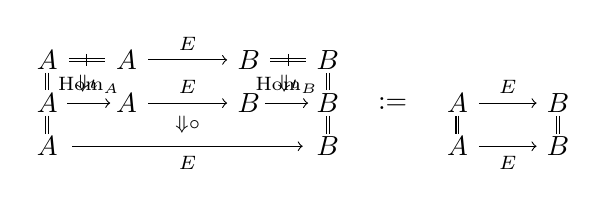
\begin{tikzpicture}[x=1.3em,y=1.3em]
  \node at (0,2.4) {$A$};
  \node at (2.2,2.4) {$A$};
  \node at (5.6,2.4) {$B$};
  \node at (7.8,2.4) {$B$};
  \draw[double] (0.6,2.4) -- (1.6,2.4);\draw (1.1,2.57) -- (1.1,2.23);
  \draw[double] (6.2,2.4) -- (7.2,2.4);\draw (6.7,2.57) -- (6.7,2.23);
  \draw[->] (2.8,2.4) -- node[above]{$\scriptstyle E$} (5.0,2.4);
  \node at (1.1,1.75) {$\scriptstyle\Downarrow\iota$};
  \node at (6.7,1.75) {$\scriptstyle\Downarrow\iota$};
  \node at (0,1.2) {$A$};
  \node at (2.2,1.2) {$A$};
  \node at (5.6,1.2) {$B$};
  \node at (7.8,1.2) {$B$};
  \draw[->] (0.55,1.2) -- node[above]{$\scriptstyle \HomA$} (1.75,1.2);
  \draw[->] (2.8,1.2) -- node[above]{$\scriptstyle E$} (5.0,1.2);
  \draw[->] (6.05,1.2) -- node[above]{$\scriptstyle \HomB$} (7.25,1.2);
  \node at (3.9,0.6) {$\scriptstyle\Downarrow\circ$};
  \node at (0,0) {$A$};
  \node at (7.8,0) {$B$};
  \draw[->] (0.7,0) -- node[below]{$\scriptstyle E$} (7.1,0);
  \draw[double] (0,2.05) -- (0,1.55);
  \draw[double] (0,0.85) -- (0,0.35);
  \draw[double] (7.8,2.05) -- (7.8,1.55);
  \draw[double] (7.8,0.85) -- (7.8,0.35);
  \node at (9.6,1.2) {$:=$};
  \node at (11.4,1.2) {$A$};
  \node at (14.2,1.2) {$B$};
  \draw[->] (12.0,1.2) -- node[above]{$\scriptstyle E$} (13.6,1.2);
  \draw[double] (11.4,0.85) -- (11.4,0.35);
  \draw[double] (14.2,0.85) -- (14.2,0.35);
  \node at (11.4,0) {$A$};
  \node at (14.2,0) {$B$};
  \draw[->] (12.0,0) -- node[below]{$\scriptstyle E$} (13.6,0);
\end{tikzpicture}
\end{center}
将 $E$ 展示为强复合 $\HomA\otimes E\otimes \HomB$。
\end{lemma}

\begin{proof}
本结果由\cref{lem:strong-composite-associativity}(ii) 与%
\cref{lem:trivial-composites}立得。
\end{proof}

\begin{proposition}\label{prop:composite-of-legs}
设 $A\xrightarrow{E}B$ 是由\trSpan{}
$A\overset{q}{\twoheadleftarrow}E\overset{p}{\twoheadrightarrow}B$ 编码的一个
模。那么，由定理 7.1.4(iii) 的\trLeftAdjoint{}与\trRightAdjoint{}之复合所表
示的二元模映射
\begin{center}
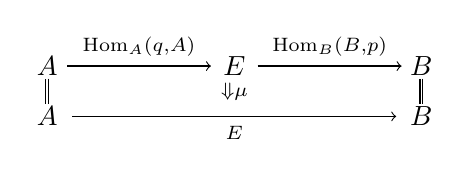
\begin{tikzpicture}[x=1.3em,y=1.3em]
  \node at (0,1.4) {$A$};
  \node at (5.2,1.4) {$E$};
  \node at (10.4,1.4){$B$};
  \draw[->] (0.55,1.4) -- node[above]{$\scriptstyle \HomA(q,A)$} (4.55,1.4);
  \draw[->] (5.85,1.4) -- node[above]{$\scriptstyle \HomB(B,p)$} (9.85,1.4);
  \draw[double] (0,1.05) -- (0,0.35);
  \draw[double] (10.4,1.05) -- (10.4,0.35);
  \node at (5.2,0.7) {$\scriptstyle\Downarrow\mu$};
  \node at (0,0) {$A$};
  \node at (10.4,0){$B$};
  \draw[->] (0.7,0) -- node[below]{$\scriptstyle E$} (9.7,0);
\end{tikzpicture}
\end{center}
展示一个强复合 $\HomA(q,A)\otimes \HomB(B,p)\simeq E$，它把该模表达为代表其
两腿的那些模的复合。
\end{proposition}

\begin{proof}
本结果由定理 7.1.4(iii) 与\cref{lem:fibered-adjoint-strong-composite}（用两
次）立得。\footnote{当然，一个\trLeftAdjoint{}与一个\trRightAdjoint{}的复合
并不是伴随，但这里我们实质上复合的是伴随等价，此时方向无关紧要。}
\end{proof}

\begin{remark}\label{rem:two-sided-fibration-version}
\cref{prop:composite-of-legs}的证明中没有任何一处要求\trSpan{}
$A\overset{q}{\twoheadleftarrow}E\overset{p}{\twoheadrightarrow}B$ 真的是一个
模，而不只是一个单纯的双侧纤维化——唯一的例外是把 $\mu$ 解读为模的%
\trVirtualEquipment{}中的一个二元\trCell。对任意双侧纤维化
$A\overset{q}{\twoheadleftarrow}E\overset{p}{\twoheadrightarrow}B$，沿\trSpan{}%
映射 $\ulcorner\mu\urcorner$ 作限制仍然定义一个双射，其一边是源包含\trSpan{}%
$E$ 且余定义域为模的那些双侧等价纤维化映射，另一边是源转而包含
$\HomA(q,A)\divideontimes \HomB(B,p)$ 的那些映射。特别地，对从 $A$ 到 $B$ 的任意相
容模序列 $E_{1}\divideontimes\cdots\divideontimes E_{n}$，只要其跨度复合定义了双侧纤维化
$A\overset{q}{\twoheadleftarrow}\vec{E}\overset{p}{\twoheadrightarrow}B$，在
模的\trVirtualEquipment{}中的诸模映射之间就存在一个双射\footnote{下右图
中央顶点原书印作 $\vec{E}$。按记号 8.2.7，$\vec{E}$ 表相容序列的复合双侧%
纤维化，而此处顶点应是两支 hom 模 $\HomA(q,A)$ 与 $\HomB(B,p)$ 相会之
对象 $E$，疑原书衍一笔画，此处径改。——译者注}：
\begin{center}
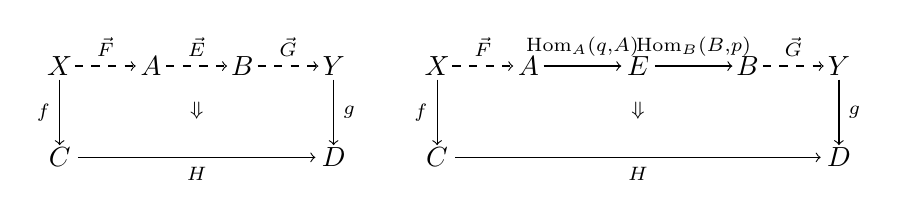
\begin{tikzpicture}[x=1.1em,y=1.1em]
  \node at (0,1.6) {$X$};
  \node at (3.0,1.6) {$A$};
  \node at (6.0,1.6) {$B$};
  \node at (9.0,1.6) {$Y$};
  \draw[->,dashed] (0.5,1.6) -- node[above]{$\scriptstyle\vec{F}$} (2.5,1.6);
  \draw[->,dashed] (3.5,1.6) -- node[above]{$\scriptstyle\vec{E}$} (5.5,1.6);
  \draw[->,dashed] (6.5,1.6) -- node[above]{$\scriptstyle\vec{G}$} (8.5,1.6);
  \node at (4.5,0.15) {$\scriptstyle\Downarrow$};
  \node at (0,-1.4) {$C$};
  \node at (9.0,-1.4){$D$};
  \draw[->] (0,1.15) -- node[left]{$\scriptstyle f$} (0,-1.0);
  \draw[->] (9.0,1.15) -- node[right]{$\scriptstyle g$} (9.0,-1.0);
  \draw[->] (0.6,-1.4) -- node[below]{$\scriptstyle H$} (8.4,-1.4);
  \node at (10.7,0.1) {$\leftrightsquigarrow$};
  \begin{scope}[shift={(12.4,0)}]
  \node at (0,1.6) {$X$};
  \node at (3.0,1.6) {$A$};
  \node at (6.6,1.6) {$E$};
  \node at (10.2,1.6){$B$};
  \node at (13.2,1.6){$Y$};
  \draw[->,dashed] (0.5,1.6) -- node[above]{$\scriptstyle\vec{F}$} (2.5,1.6);
  \draw[->] (3.5,1.6) -- node[above]{$\scriptstyle \HomA(q,A)$} (6.05,1.6);
  \draw[->] (7.15,1.6) -- node[above]{$\scriptstyle \HomB(B,p)$} (9.7,1.6);
  \draw[->,dashed] (10.7,1.6) -- node[above]{$\scriptstyle\vec{G}$} (12.7,1.6);
  \node at (6.6,0.15) {$\scriptstyle\Downarrow$};
  \node at (0,-1.4) {$C$};
  \node at (13.2,-1.4){$D$};
  \draw[->] (0,1.15) -- node[left]{$\scriptstyle f$} (0,-1.0);
  \draw[->] (13.2,1.15) -- node[right]{$\scriptstyle g$} (13.2,-1.0);
  \draw[->] (0.6,-1.4) -- node[below]{$\scriptstyle H$} (12.6,-1.4);
  \end{scope}
\end{tikzpicture}
\end{center}
\end{remark}

\begin{remark}\label{rem:comma-cone-description}
\cref{prop:composite-of-legs}与\cref{rem:two-sided-fibration-version}中的复
合映射 $\mu\colon \HomA(q,A)\divideontimes \HomB(B,p)\Rightarrow E$ 可以用另一种方
式来描述。$\HomA(q,A)$ 与 $\HomB(B,p)$ 的诸\trCommaCone{}定义了一对自然变
换，定理 7.1.4(iv) 的前提适用于它们。
\begin{center}
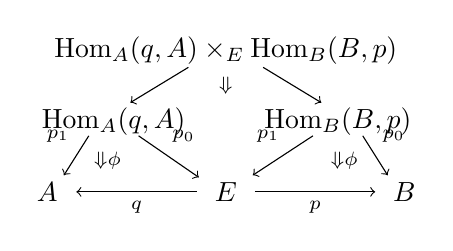
\begin{tikzpicture}[x=1.5em,y=1.5em]
  \node at (0,3.4) {$\HomA(q,A)\times_{E} \HomB(B,p)$};
  \node at (-2.7,1.7) {$\HomA(q,A)$};
  \node at (2.7,1.7) {$\HomB(B,p)$};
  \draw[->] (-0.9,3.0) -- (-2.3,2.15);
  \draw[->] (0.9,3.0) -- (2.3,2.15);
  \node at (0,2.55) {$\scriptstyle\Downarrow$};
  \node at (-4.3,0) {$A$};
  \node at (0,0) {$E$};
  \node at (4.3,0) {$B$};
  \draw[->] (-3.3,1.35) -- node[above left,pos=0.4]{$\scriptstyle p_{1}$} (-3.9,0.4);
  \draw[->] (-2.1,1.35) -- node[above right,pos=0.4]{$\scriptstyle p_{0}$} (-0.65,0.35);
  \node at (-2.85,0.75) {$\scriptstyle\Downarrow\phi$};
  \draw[->] (2.1,1.35) -- node[above left,pos=0.4]{$\scriptstyle p_{1}$} (0.65,0.4);
  \draw[->] (3.3,1.35) -- node[above right,pos=0.4]{$\scriptstyle p_{0}$} (3.9,0.4);
  \node at (2.85,0.75) {$\scriptstyle\Downarrow\phi$};
  \draw[->] (-0.7,0) -- node[below]{$\scriptstyle q$} (-3.6,0);
  \draw[->] (0.7,0) -- node[below]{$\scriptstyle p$} (3.6,0);
\end{tikzpicture}
\end{center}
该结果的结论断言：存在一个良定义的、诸\trFunctor{}的纤维化同构类
$\ulcorner\mu\urcorner\colon \HomA(q,A)\times_{E}\HomB(B,p)\to E$，其定义
是：取左\trCommaCone{}的 $q$-余笛卡尔提升，与右\trCommaCone{}复合，然后取这
一复合\trCell{}的某个 $p$-笛卡尔提升的余定义域——或者先取 $p$-笛卡尔提升，
复合，然后取这一复合的某个 $q$-笛卡尔提升的定义域——此即定理 7.1.4(iii) 记
法下的\trFunctor{} $\ell r\simeq r\ell$。在 $A\xrightarrow{E}B$ 本身是一个逗
号模的情形，所得的诸\trFunctor{}的纤维化同构类 $\ulcorner\mu\urcorner$ 恰是
对如下 2-胞腔进行分类的那一个：该 2-胞腔由所示复合与位于 $E$ 之下的%
\trCommaCone{}粘贴而成。
\end{remark}

任何\trVirtualDoubleCategory{}对每支水平箭头 $A\xrightarrow{E}B$ 都有一个竖直
恒同\trCell，其竖直边界箭头为恒同。在一个\trVirtualEquipment{}中，我们对每支
竖直箭头 $f\colon A\to B$ 还有一个水平一元\textbf{单位\trCell}（unit cell），
其水平边界由命题 8.2.4 的诸单位模 $A\xrightarrow{\HomA}A$ 与
$B\xrightarrow{\HomB}B$ 给出。

\begin{definition}\label{def:unary-unit-cell}
利用 $\Mod(\mathcal{K})$ 中的诸单位模，对任意\trFunctor{} $f\colon A\to B$，
我们可以借助 $A$ 处的零元单位\trCell{}
$\iota\colon\varnothing\Rightarrow \HomA$ 的\trUniversalProperty，通过下右图
的等式来定义如下左图所示的一元单位\trCell：
\begin{center}
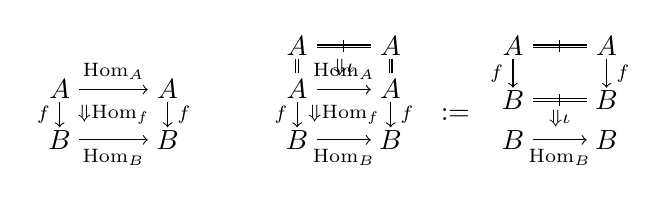
\begin{tikzpicture}[x=1.3em,y=1.3em]
  \node at (0,1.4) {$A$};
  \node at (3.0,1.4) {$A$};
  \draw[->] (0.55,1.4) -- node[above]{$\scriptstyle \HomA$} (2.45,1.4);
  \draw[->] (0,1.05) -- node[left]{$\scriptstyle f$} (0,0.35);
  \draw[->] (3.0,1.05) -- node[right]{$\scriptstyle f$} (3.0,0.35);
  \node at (1.5,0.7) {$\scriptstyle\Downarrow \Homf$};
  \node at (0,0) {$B$};
  \node at (3.0,0) {$B$};
  \draw[->] (0.55,0) -- node[below]{$\scriptstyle \HomB$} (2.45,0);
  \node at (4.7,0.7) {$\leftrightsquigarrow$};
  \begin{scope}[shift={(6.6,0)}]
  \node at (0,2.6) {$A$};
  \node at (2.6,2.6) {$A$};
  \draw[double] (0.55,2.6) -- (2.05,2.6);\draw (1.3,2.77) -- (1.3,2.43);
  \draw[double] (0,2.25) -- (0,1.85);
  \draw[double] (2.6,2.25) -- (2.6,1.85);
  \node at (1.3,2.02) {$\scriptstyle\Downarrow\iota$};
  \node at (0,1.4) {$A$};
  \node at (2.6,1.4) {$A$};
  \draw[->] (0.55,1.4) -- node[above]{$\scriptstyle \HomA$} (2.05,1.4);
  \draw[->] (0,1.05) -- node[left]{$\scriptstyle f$} (0,0.35);
  \draw[->] (2.6,1.05) -- node[right]{$\scriptstyle f$} (2.6,0.35);
  \node at (1.3,0.7) {$\scriptstyle\Downarrow \Homf$};
  \node at (0,0) {$B$};
  \node at (2.6,0) {$B$};
  \draw[->] (0.55,0) -- node[below]{$\scriptstyle \HomB$} (2.05,0);
  \end{scope}
  \node at (11.0,0.7) {$:=$};
  \begin{scope}[shift={(12.6,0)}]
  \node at (0,2.6) {$A$};
  \node at (2.6,2.6) {$A$};
  \draw[double] (0.55,2.6) -- (2.05,2.6);\draw (1.3,2.77) -- (1.3,2.43);
  \draw[->] (0,2.25) -- node[left]{$\scriptstyle f$} (0,1.45);
  \draw[->] (2.6,2.25) -- node[right]{$\scriptstyle f$} (2.6,1.45);
  \node at (0,1.1) {$B$};
  \node at (2.6,1.1) {$B$};
  \draw[double] (0.55,1.1) -- (2.05,1.1);\draw (1.3,1.27) -- (1.3,0.93);
  \node at (1.3,0.58) {$\scriptstyle\Downarrow\iota$};
  \node at (0,0) {$B$};
  \node at (2.6,0) {$B$};
  \draw[->] (0.55,0) -- node[below]{$\scriptstyle \HomB$} (2.05,0);
  \end{scope}
\end{tikzpicture}
\end{center}
\end{definition}

在引理 8.1.16 的刻画中，定义一元单位\trCell{}的粘贴等式的两边都对应于如下所
示的恒同 2-胞腔：
\begin{center}
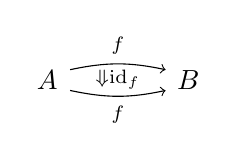
\begin{tikzpicture}[x=1.5em,y=1.5em]
  \node at (0,0.9) {$A$};
  \node at (3.4,0.9) {$B$};
  \draw[->] (0.55,1.15) to[bend left=12] node[above]{$\scriptstyle f$} (2.85,1.15);
  \draw[->] (0.55,0.65) to[bend right=12] node[below]{$\scriptstyle f$} (2.85,0.65);
  \node at (1.7,0.9) {$\scriptstyle\Downarrow\mathrm{id}_{f}$};
\end{tikzpicture}
\end{center}

一如所愿，在模的\trVirtualEquipment{}中，诸单位\trCell{}是诸\trCell{}的竖直
复合的单位。

\begin{lemma}[与单位\trCell{}的复合]\label{lem:composition-with-unit-cells}
任何如下右图所示的\trCell{} $\alpha$ 都等于如下左图所示的粘贴复合\footnote{%
原书引理 8.3.15 的两对粘贴图（本图与证明图，p.328--329）的四条 $B\to C$ 底边均
印作 $\vec{E}$。按记号 8.2.7，$\vec{E}$ 专指序列
$E_{1}\divideontimes\cdots\divideontimes E_{n}$（$A_{0}\to A_{n}$ 方向）的复合
双侧纤维化，标于 $B\to C$ 之边无义；且外侧胞腔之靶即 $\circ$ 之靶（由引理
8.3.10，$\circ$ 之靶为模 $E\colon B\to C$），恒同胞腔之分解亦要求上下边相%
一致。四处径改。——译者注}：
\begin{center}
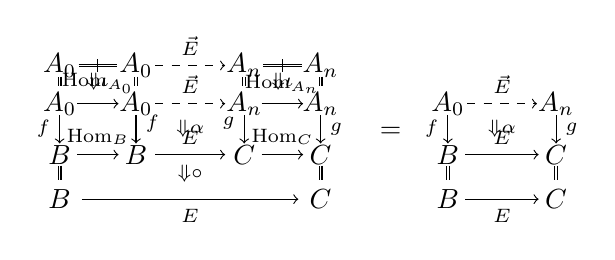
\begin{tikzpicture}[x=1.15em,y=1.15em]
  \node at (0,3.6) {$A_{0}$};
  \node at (2.4,3.6) {$A_{0}$};
  \node at (5.8,3.6) {$A_{n}$};
  \node at (8.2,3.6) {$A_{n}$};
  \draw[double] (0.6,3.6) -- (1.8,3.6);\draw (1.2,3.79) -- (1.2,3.41);
  \draw[double] (6.4,3.6) -- (7.6,3.6);\draw (7.0,3.79) -- (7.0,3.41);
  \draw[->,dashed] (3.0,3.6) -- node[above]{$\scriptstyle\vec{E}$} (5.2,3.6);
  \draw[double] (0,3.25) -- (0,2.95);
  \draw[double] (2.4,3.25) -- (2.4,2.95);
  \draw[double] (5.8,3.25) -- (5.8,2.95);
  \draw[double] (8.2,3.25) -- (8.2,2.95);
  \node at (1.2,3.1) {$\scriptstyle\Downarrow\iota$};
  \node at (7.0,3.1) {$\scriptstyle\Downarrow\iota$};
  \node at (0,2.4) {$A_{0}$};
  \node at (2.4,2.4) {$A_{0}$};
  \node at (5.8,2.4) {$A_{n}$};
  \node at (8.2,2.4) {$A_{n}$};
  \draw[->] (0.55,2.4) -- node[above]{$\scriptstyle \mathrm{Hom}_{A_{0}}$} (1.85,2.4);
  \draw[->,dashed] (3.0,2.4) -- node[above]{$\scriptstyle\vec{E}$} (5.2,2.4);
  \draw[->] (6.35,2.4) -- node[above]{$\scriptstyle \mathrm{Hom}_{A_{n}}$} (7.65,2.4);
  \draw[->] (0,2.05) -- node[left]{$\scriptstyle f$} (0,1.15);
  \draw[->] (2.4,2.05) -- node[right,pos=0.3]{$\scriptstyle f$} (2.4,1.15);
  \node at (4.1,1.6) {$\scriptstyle\Downarrow\alpha$};
  \draw[->] (5.8,2.05) -- node[left,pos=0.3]{$\scriptstyle g$} (5.8,1.15);
  \draw[->] (8.2,2.05) -- node[right]{$\scriptstyle g$} (8.2,1.15);
  \node at (0,0.8) {$B$};
  \node at (2.4,0.8) {$B$};
  \node at (5.8,0.8) {$C$};
  \node at (8.2,0.8) {$C$};
  \draw[->] (0.55,0.8) -- node[above]{$\scriptstyle \HomB$} (1.85,0.8);
  \draw[->] (3.0,0.8) -- node[above]{$\scriptstyle E$} (5.2,0.8);
  \draw[->] (6.35,0.8) -- node[above]{$\scriptstyle \HomC$} (7.65,0.8);
  \node at (4.1,0.2) {$\scriptstyle\Downarrow\circ$};
  \draw[double] (0,0.45) -- (0,0.0);
  \draw[double] (8.2,0.45) -- (8.2,0.0);
  \node at (0,-0.6) {$B$};
  \node at (8.2,-0.6){$C$};
  \draw[->] (0.7,-0.6) -- node[below]{$\scriptstyle E$} (7.5,-0.6);
  \node at (10.4,1.5) {$=$};
  \begin{scope}[shift={(12.2,0)}]
  \node at (0,2.4) {$A_{0}$};
  \node at (3.4,2.4) {$A_{n}$};
  \draw[->,dashed] (0.6,2.4) -- node[above]{$\scriptstyle\vec{E}$} (2.8,2.4);
  \draw[->] (0,2.05) -- node[left]{$\scriptstyle f$} (0,1.15);
  \draw[->] (3.4,2.05) -- node[right]{$\scriptstyle g$} (3.4,1.15);
  \node at (1.7,1.6) {$\scriptstyle\Downarrow\alpha$};
  \node at (0,0.8) {$B$};
  \node at (3.4,0.8) {$C$};
  \draw[->] (0.55,0.8) -- node[above]{$\scriptstyle E$} (2.85,0.8);
  \draw[double] (0,0.45) -- (0,0.0);
  \draw[double] (3.4,0.45) -- (3.4,0.0);
  \node at (0,-0.6) {$B$};
  \node at (3.4,-0.6){$C$};
  \draw[->] (0.55,-0.6) -- node[below]{$\scriptstyle E$} (2.85,-0.6);
  \end{scope}
\end{tikzpicture}
\end{center}
\end{lemma}

\begin{proof}
由\cref{def:unary-unit-cell}与定义 8.1.8 所陈述的、\trVirtualDoubleCategory{}%
中与恒同\trCell{}复合的诸定律，所述等式的左边复合等于下面展示的左边复合%
\trCell，而所述等式的右边等于下面展示的右边复合\trCell：
\begin{center}
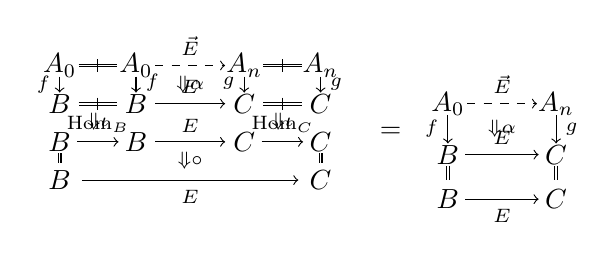
\begin{tikzpicture}[x=1.15em,y=1.15em]
  \node at (0,3.6) {$A_{0}$};
  \node at (2.4,3.6) {$A_{0}$};
  \node at (5.8,3.6) {$A_{n}$};
  \node at (8.2,3.6) {$A_{n}$};
  \draw[double] (0.6,3.6) -- (1.8,3.6);\draw (1.2,3.79) -- (1.2,3.41);
  \draw[double] (6.4,3.6) -- (7.6,3.6);\draw (7.0,3.79) -- (7.0,3.41);
  \draw[->,dashed] (3.0,3.6) -- node[above]{$\scriptstyle\vec{E}$} (5.2,3.6);
  \draw[->] (0,3.25) -- node[left]{$\scriptstyle f$} (0,2.75);
  \draw[->] (2.4,3.25) -- node[right,pos=0.4]{$\scriptstyle f$} (2.4,2.75);
  \node at (4.1,3.0) {$\scriptstyle\Downarrow\alpha$};
  \draw[->] (5.8,3.25) -- node[left,pos=0.4]{$\scriptstyle g$} (5.8,2.75);
  \draw[->] (8.2,3.25) -- node[right]{$\scriptstyle g$} (8.2,2.75);
  \node at (0,2.4) {$B$};
  \node at (2.4,2.4) {$B$};
  \node at (5.8,2.4) {$C$};
  \node at (8.2,2.4) {$C$};
  \draw[double] (0.6,2.4) -- (1.8,2.4);\draw (1.2,2.59) -- (1.2,2.21);
  \draw[->] (3.0,2.4) -- node[above]{$\scriptstyle E$} (5.2,2.4);
  \draw[double] (6.4,2.4) -- (7.6,2.4);\draw (7.0,2.59) -- (7.0,2.21);
  \node at (1.2,1.85) {$\scriptstyle\Downarrow\iota$};
  \node at (7.0,1.85) {$\scriptstyle\Downarrow\iota$};
  \node at (0,1.2) {$B$};
  \node at (2.4,1.2) {$B$};
  \node at (5.8,1.2) {$C$};
  \node at (8.2,1.2) {$C$};
  \draw[->] (0.55,1.2) -- node[above]{$\scriptstyle \HomB$} (1.85,1.2);
  \draw[->] (3.0,1.2) -- node[above]{$\scriptstyle E$} (5.2,1.2);
  \draw[->] (6.35,1.2) -- node[above]{$\scriptstyle \HomC$} (7.65,1.2);
  \node at (4.1,0.6) {$\scriptstyle\Downarrow\circ$};
  \draw[double] (0,0.85) -- (0,0.55);
  \draw[double] (8.2,0.85) -- (8.2,0.55);
  \node at (0,0) {$B$};
  \node at (8.2,0) {$C$};
  \draw[->] (0.7,0) -- node[below]{$\scriptstyle E$} (7.5,0);
  \node at (10.4,1.5) {$=$};
  \begin{scope}[shift={(12.2,0)}]
  \node at (0,2.4) {$A_{0}$};
  \node at (3.4,2.4) {$A_{n}$};
  \draw[->,dashed] (0.6,2.4) -- node[above]{$\scriptstyle\vec{E}$} (2.8,2.4);
  \draw[->] (0,2.05) -- node[left]{$\scriptstyle f$} (0,1.15);
  \draw[->] (3.4,2.05) -- node[right]{$\scriptstyle g$} (3.4,1.15);
  \node at (1.7,1.6) {$\scriptstyle\Downarrow\alpha$};
  \node at (0,0.8) {$B$};
  \node at (3.4,0.8) {$C$};
  \draw[->] (0.55,0.8) -- node[above]{$\scriptstyle E$} (2.85,0.8);
  \draw[double] (0,0.45) -- (0,0.0);
  \draw[double] (3.4,0.45) -- (3.4,0.0);
  \node at (0,-0.6) {$B$};
  \node at (3.4,-0.6){$C$};
  \draw[->] (0.55,-0.6) -- node[below]{$\scriptstyle E$} (2.85,-0.6);
  \end{scope}
\end{tikzpicture}
\end{center}
由\cref{lem:composites-with-units}，左边等于右边。
\end{proof}

\begin{definition}[胞腔的水平复合]\label{def:horizontal-composite-cells}
若给定一个水平相容的一元\trCell{}序列
\begin{center}
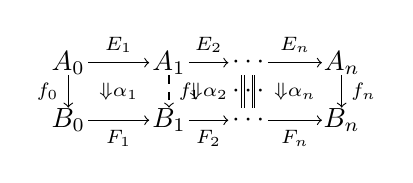
\begin{tikzpicture}[x=1.3em,y=1.3em]
  \node at (0,1.6) {$A_{0}$};
  \node at (2.8,1.6) {$A_{1}$};
  \node at (5.0,1.6) {$\cdots$};
  \node at (7.6,1.6) {$A_{n}$};
  \draw[->] (0.55,1.6) -- node[above]{$\scriptstyle E_{1}$} (2.25,1.6);
  \draw[->] (3.35,1.6) -- node[above]{$\scriptstyle E_{2}$} (4.45,1.6);
  \draw[->] (5.55,1.6) -- node[above]{$\scriptstyle E_{n}$} (7.05,1.6);
  \draw[->] (0,1.25) -- node[left]{$\scriptstyle f_{0}$} (0,0.35);
  \node at (1.4,0.8) {$\scriptstyle\Downarrow\alpha_{1}$};
  \draw[->,dashed] (2.8,1.25) -- node[right]{$\scriptstyle f_{1}$} (2.8,0.35);
  \node at (3.9,0.8) {$\scriptstyle\Downarrow\alpha_{2}$};
  \draw[double] (4.85,1.25) -- (4.85,0.35);
  \draw[double] (5.15,1.25) -- (5.15,0.35);
  \node at (5.0,0.8) {$\cdots$};
  \node at (6.3,0.8) {$\scriptstyle\Downarrow\alpha_{n}$};
  \draw[->] (7.6,1.25) -- node[right]{$\scriptstyle f_{n}$} (7.6,0.35);
  \node at (0,0) {$B_{0}$};
  \node at (2.8,0) {$B_{1}$};
  \node at (5.0,0) {$\cdots$};
  \node at (7.6,0) {$B_{n}$};
  \draw[->] (0.55,0) -- node[below]{$\scriptstyle F_{1}$} (2.25,0);
  \draw[->] (3.35,0) -- node[below]{$\scriptstyle F_{2}$} (4.45,0);
  \draw[->] (5.55,0) -- node[below]{$\scriptstyle F_{n}$} (7.05,0);
\end{tikzpicture}
\end{center}
使得相容序列 $E_{1}\divideontimes\cdots\divideontimes E_{n}$ 与
$F_{1}\divideontimes\cdots\divideontimes F_{n}$ 都容许复合，那么就存在一个\textbf{水平复合
一元\trCell}（horizontal composite unary cell）
$\alpha_{1}*\cdots *\alpha_{n}$，它在给定复合
$\circ\colon E_{1}\divideontimes\cdots\divideontimes E_{n}\Rightarrow E$ 与
$F_{1}\divideontimes\cdots\divideontimes F_{n}\Rightarrow F$ 的取法之下，由如下粘贴等式唯
一确定：
\begin{rveq}\label{eq:horizontal-composite-pasting}
\begin{tikzpicture}[x=1.3em,y=1.3em]
  \node at (0,2.6) {$A_{0}$};
  \node at (2.8,2.6) {$A_{1}$};
  \node at (5.0,2.6) {$\cdots$};
  \node at (7.6,2.6) {$A_{n}$};
  \draw[->] (0.55,2.6) -- node[above]{$\scriptstyle E_{1}$} (2.25,2.6);
  \draw[->] (3.35,2.6) -- node[above]{$\scriptstyle E_{2}$} (4.45,2.6);
  \draw[->] (5.55,2.6) -- node[above]{$\scriptstyle E_{n}$} (7.05,2.6);
  \draw[double] (0,2.25) -- (0,1.75);
  \draw[double] (7.6,2.25) -- (7.6,1.75);
  \node at (3.8,1.95) {$\scriptstyle\Downarrow\circ$};
  \node at (0,1.4) {$A_{0}$};
  \node at (7.6,1.4) {$A_{n}$};
  \draw[->] (0.55,1.4) -- node[above]{$\scriptstyle E$} (7.05,1.4);
  \draw[->] (0,1.05) -- node[left]{$\scriptstyle f_{0}$} (0,0.35);
  \node at (3.8,0.7) {$\scriptstyle\Downarrow\alpha_{1}*\cdots *\alpha_{n}$};
  \draw[->] (7.6,1.05) -- node[right]{$\scriptstyle f_{n}$} (7.6,0.35);
  \node at (0,0) {$B_{0}$};
  \node at (7.6,0) {$B_{n}$};
  \draw[->] (0.55,0) -- node[below]{$\scriptstyle F$} (7.05,0);
  \node at (9.4,1.2) {$:=$};
  \begin{scope}[shift={(11.2,0)}]
  \node at (0,2.6) {$A_{0}$};
  \node at (2.8,2.6) {$A_{1}$};
  \node at (5.0,2.6) {$\cdots$};
  \node at (7.6,2.6) {$A_{n}$};
  \draw[->] (0.55,2.6) -- node[above]{$\scriptstyle E_{1}$} (2.25,2.6);
  \draw[->] (3.35,2.6) -- node[above]{$\scriptstyle E_{2}$} (4.45,2.6);
  \draw[->] (5.55,2.6) -- node[above]{$\scriptstyle E_{n}$} (7.05,2.6);
  \draw[->] (0,2.25) -- node[left]{$\scriptstyle f_{0}$} (0,1.75);
  \node at (1.4,1.95) {$\scriptstyle\Downarrow\alpha_{1}$};
  \draw[->,dashed] (2.8,2.25) -- node[right]{$\scriptstyle f_{1}$} (2.8,1.75);
  \node at (3.9,1.95) {$\scriptstyle\Downarrow\alpha_{2}$};
  \draw[double] (4.85,2.25) -- (4.85,1.75);
  \draw[double] (5.15,2.25) -- (5.15,1.75);
  \node at (5.0,1.95) {$\cdots$};
  \node at (6.3,1.95) {$\scriptstyle\Downarrow\alpha_{n}$};
  \draw[->] (7.6,2.25) -- node[right]{$\scriptstyle f_{n}$} (7.6,1.75);
  \node at (0,1.4) {$B_{0}$};
  \node at (2.8,1.4) {$B_{1}$};
  \node at (5.0,1.4) {$\cdots$};
  \node at (7.6,1.4) {$B_{n}$};
  \draw[->] (0.55,1.4) -- node[above]{$\scriptstyle F_{1}$} (2.25,1.4);
  \draw[->] (3.35,1.4) -- node[above]{$\scriptstyle F_{2}$} (4.45,1.4);
  \draw[->] (5.55,1.4) -- node[above]{$\scriptstyle F_{n}$} (7.05,1.4);
  \draw[double] (0,1.05) -- (0,0.55);
  \draw[double] (7.6,1.05) -- (7.6,0.55);
  \node at (3.8,0.8) {$\scriptstyle\Downarrow\circ$};
  \node at (0,0) {$B_{0}$};
  \node at (7.6,0) {$B_{n}$};
  \draw[->] (0.55,0) -- node[below]{$\scriptstyle F$} (7.05,0);
  \end{scope}
\end{tikzpicture}
\end{rveq}
\end{definition}

通过一个与\cref{lem:composition-with-unit-cells}之证明十分类似的论证（其中
用到\cref{lem:composites-with-units}的诸复合），一元\trCell{} $\alpha$ 与位
于其竖直边界\trFunctor{}处的单位\trCell{} $\Homf$ 与 $\Homg$ 的水平复合
$\Homf*\alpha*\Homg$ 复原了 $\alpha$（见\cref{ex:unit-cells-recover-alpha}）。
利用\cref{def:horizontal-composite-cells}的一元\trCell{}水平复合，我们可以
把 $\Mod(\mathcal{K})$ 理解为包含各种「竖直的」与「水平的」\trBicategory。

\begin{proposition}[虚拟装备中的竖直 2-范畴]\label{prop:vertical-two-category}
任何\trVirtualEquipment{}都包含一个\textbf{竖直 2-范畴}（vertical
2-category）：其对象是该\trVirtualEquipment{}的对象，其箭头是竖直箭头，其
2-胞腔是如下所示的那些一元\trCell——即水平边界箭头由诸单位模给出的那些：
\begin{center}
\begin{tikzpicture}[x=1.5em,y=1.5em]
  \node at (0,1.4) {$A$};
  \node at (3.0,1.4) {$A$};
  \draw[->] (0.55,1.4) -- node[above]{$\scriptstyle \HomA$} (2.45,1.4);
  \draw[->] (0,1.05) -- node[left]{$\scriptstyle g$} (0,0.35);
  \draw[->] (3.0,1.05) -- node[right]{$\scriptstyle f$} (3.0,0.35);
  \node at (1.5,0.7) {$\scriptstyle\Downarrow\alpha$};
  \node at (0,0) {$B$};
  \node at (3.0,0) {$B$};
  \draw[->] (0.55,0) -- node[below]{$\scriptstyle \HomB$} (2.45,0);
\end{tikzpicture}
\end{center}
\end{proposition}

\begin{proof}
为证明这些结构定义一个 2-范畴，我们必须——采用定义 B.1.1 的标准术语——定
义 2-胞腔的「水平」复合（沿一个边界 0-\trCell{}复合）与「竖直」复合（沿一个
边界 1-\trCell{}复合）。2-范畴中的「水平」复合经由\trVirtualDoubleCategory{}%
中的竖直复合来定义，后者见定义 8.1.8；2-范畴中的「竖直」复合则由%
\cref{def:horizontal-composite-cells}定义。为看出所得者是 2-范畴而非\trBicategory，请注意：任何 1-胞腔的复合严格结合且严格幺的\trBicategory{}都是 2-范畴；而在此
处，1-胞腔是该\trVirtualDoubleCategory{}的竖直箭头，它们确实严格复合。
\end{proof}

在命题 8.4.11 中我们将证明：\trVirtualEquipment{} $\Mod(\mathcal{K})$ 中的竖
直 2-范畴同构于\trHomotopyTwoCategory{} $\mathfrak{h}\mathcal{K}$。

\begin{remark}[虚拟装备中的水平\trBicategory]\label{rem:horizontal-bicategories}
经由\cref{def:horizontal-composite-cells}，一个\trVirtualEquipment{}也可以被
理解为包含各种「水平的」\trBicategory：取 1-胞腔为诸可复合模，取 2-胞腔为竖直边
界\trFunctor{}为恒同的一元模映射。若干令人感兴趣的水平\trBicategory{}将在定义
8.4.12 中描述。
\end{remark}

\subsection*{练习}

\begin{exercise}\label{ex:virtual-double-composites}
推广练习 8.1.ii：证明在一个由真实\trDoubleCategory{}产生的%
\trVirtualDoubleCategory{}中，每个水平箭头的相容序列都容许\cref{def:composite}%
意义下的一个复合。
\end{exercise}

\begin{exercise}[\cite{bib53}，8.5；\cite{bib76}，3.3.4]\label{ex:all-composites}
\begin{enumerate}[label=(\roman*)]
\item 设在一个\trVirtualEquipment{}中，对每个相容序列
$E_{1}\divideontimes\cdots\divideontimes E_{n}$ 都存在一个\trCell{}
$\mu\colon E_{1}\divideontimes\cdots\divideontimes E_{n}\Rightarrow E$，它是\emph{弱余笛卡
尔的}（weakly cocartesian），意即每个 $n$ 元\trCell{}
$E_{1}\divideontimes\cdots\divideontimes E_{n}\Rightarrow H$ 都经由一个一元\trCell{}
$E\Rightarrow H$ 唯一地穿过 $\mu$ 而分解。若再者诸弱余笛卡尔的\trCell{}在该%
\trVirtualDoubleCategory{}中对复合封闭，请证明每个弱余笛卡尔的\trCell{}实际
上是余笛卡尔的，即满足\cref{def:composite}的\trUniversalProperty，并据此断
言：此时该\trVirtualEquipment{}容许所有复合。
\item 设 $\mathcal{K}$ 是一个\trInfinityCosmos，其中每个双侧纤维化
$A\overset{q}{\twoheadleftarrow}E\overset{p}{\twoheadrightarrow}B$ 都能被反射
为一个模，意即存在一个\trSpan{}映射使 $\tilde{E}$ 为一个模，使得对每个模
$A\xrightarrow{H}B$，$\mu$ 都诱导 Kan 复形的\trEquivalence
\begin{center}
\begin{tikzpicture}[x=1.5em,y=1.5em]
  \node at (0,2.0) {$E$};
  \node at (-2.8,0.4) {$A$};
  \node at (2.8,0.4) {$B$};
  \node at (0,-0.9) {$\tilde{E}$};
  \draw[->] (-0.65,1.75) -- node[above left,pos=0.4]{$\scriptstyle q$} (-2.25,0.75);
  \draw[->] (0.65,1.75) -- node[above right,pos=0.4]{$\scriptstyle p$} (2.25,0.75);
  \draw[->] (0,1.6) -- node[right,pos=0.5]{$\scriptstyle\mu$} (0,-0.45);
  \draw[->] (-0.65,-1.15) -- node[below left,pos=0.4]{$\scriptstyle\tilde{q}$} (-2.25,-0.05);
  \draw[->] (0.65,-1.15) -- node[below right,pos=0.4]{$\scriptstyle\tilde{p}$} (2.25,-0.05);
  \node at (5.2,0.4) {$\rightsquigarrow$};
  \node at (10.2,0.4)
    {$\Fun_{A\times B}(\tilde{E},H)\xrightarrow[\ \simeq\ ]{\,-\circ\mu\,}\Fun_{A\times B}(E,H)$.};
\end{tikzpicture}
\end{center}
请断言：\trVirtualEquipment{} $\Mod(\mathcal{K})$ 拥有所有复合。
\end{enumerate}
\end{exercise}

\begin{exercise}\label{ex:strong-composite-associativity}
证明\cref{lem:strong-composite-associativity}。
\end{exercise}

\begin{exercise}\label{ex:trivial-composites-proof}
证明\cref{lem:trivial-composites}。
\end{exercise}

\begin{exercise}\label{ex:unit-cells-recover-alpha}
对任意如下所示的一元\trCell，证明水平复合 $\Homf*\alpha*\Homg$ 等于 $\alpha$。
\begin{center}
\begin{tikzpicture}[x=1.5em,y=1.5em]
  \node at (0,1.4) {$A$};
  \node at (3.0,1.4) {$B$};
  \draw[->] (0.55,1.4) -- node[above]{$\scriptstyle E$} (2.45,1.4);
  \draw[->] (0,1.05) -- node[left]{$\scriptstyle f$} (0,0.35);
  \draw[->] (3.0,1.05) -- node[right]{$\scriptstyle g$} (3.0,0.35);
  \node at (1.5,0.7) {$\scriptstyle\Downarrow\alpha$};
  \node at (0,0) {$C$};
  \node at (3.0,0) {$D$};
  \draw[->] (0.55,0) -- node[below]{$\scriptstyle F$} (2.45,0);
\end{tikzpicture}
\end{center}
\end{exercise}


   %
\providecommand{\Mod}{\mathbb{M}od}
\providecommand{\HomA}{\mathrm{Hom}_{A}}
\providecommand{\HomB}{\mathrm{Hom}_{B}}
\providecommand{\HomC}{\mathrm{Hom}_{C}}
\providecommand{\HomD}{\mathrm{Hom}_{D}}
\providecommand{\HomE}{\mathrm{Hom}_{E}}
\providecommand{\rvbendL}{\tikz[baseline=-0.5ex,x=0.9em,y=0.9em]%
\draw[->] (0.8,0.7) .. controls (-0.6,0.7) and (-0.6,-0.7) .. (0.8,-0.7);}
\providecommand{\rvbendR}{\tikz[baseline=-0.5ex,x=0.9em,y=0.9em]%
\draw[->] (-0.8,-0.7) .. controls (0.6,-0.7) and (0.6,0.7) .. (-0.8,0.7);}

\section{可表示模}\label{sec:representable-modules}

虚拟装备中的任何竖直箭头 $f\colon A\to B$ 都带有一对与之相关联的水平箭头
$B\xrightarrow{\HomB(f,B)}A$ 与 $A\xrightarrow{\HomB(B,f)}B$，它们定义为诸水平
单位箭头的限制，并拥有与通常\trDoubleCategory{}中的\emph{\trCompanion}（companion）与%
\emph{\trConjoint}（conjoint）相类似的\trUniversalProperty{} $[47]$。
在模的\trVirtualEquipment{}中，把它们合情理地称作一个\trFunctor{}作为模的%
\emph{左表示与右表示}（left and right representations of a functor as a module），
并沿用这套熟悉的术语与记号，因为它们恰好与定义 3.5.1 和 7.4.7 中引入的左、右
可表示元完全重合。

\begin{proposition}[可表示元的\trCompanion{}与\trConjoint{}关系]%
\label{prop:representable-restriction-application}
对于模的\trVirtualEquipment{}中的任何\trFunctor{} $f\colon A\to B$，存在%
\trCanonical{}限制胞腔（下左两图所示）与应用胞腔（下右两图所示）
\begin{center}
\begin{tikzpicture}[x=1.3em,y=1.3em]
  \node (a1) at (0,1.5)   {$B$};
  \node (a2) at (3.4,1.5) {$A$};
  \node (a3) at (0,0)     {$B$};
  \node (a4) at (3.4,0)   {$B$};
  \draw[->] (0.7,1.5) -- node[above]{$\scriptstyle\HomB(f,B)$} (2.7,1.5);
  \draw[double,double distance=0.6pt] (0,1.15) -- (0,0.35);
  \draw[->] (3.4,1.15) -- (3.4,0.35);
  \node at (3.9,0.75) {$\scriptstyle f$};
  \node at (1.7,0.75) {$\scriptstyle\Downarrow\rho$};
  \draw[->] (0.7,0) -- node[below]{$\scriptstyle\HomB$} (2.7,0);
\end{tikzpicture}
\qquad
\begin{tikzpicture}[x=1.3em,y=1.3em]
  \node (b1) at (0,1.5)   {$A$};
  \node (b2) at (3.4,1.5) {$B$};
  \node (b3) at (0,0)     {$B$};
  \node (b4) at (3.4,0)   {$B$};
  \draw[->] (0.7,1.5) -- node[above]{$\scriptstyle\HomB(B,f)$} (2.7,1.5);
  \draw[->] (0,1.15) -- (0,0.35);
  \node at (-0.5,0.75) {$\scriptstyle f$};
  \draw[double,double distance=0.6pt] (3.4,1.15) -- (3.4,0.35);
  \node at (1.7,0.75) {$\scriptstyle\Downarrow\rho$};
  \draw[->] (0.7,0) -- node[below]{$\scriptstyle\HomB$} (2.7,0);
\end{tikzpicture}
\qquad
\begin{tikzpicture}[x=1.3em,y=1.3em]
  \node (c1) at (0,1.5)   {$A$};
  \node (c2) at (3.4,1.5) {$A$};
  \node (c3) at (0,0)     {$B$};
  \node (c4) at (3.4,0)   {$A$};
  \draw[->] (0.7,1.5) -- node[above]{$\scriptstyle\HomA$} (2.7,1.5);
  \draw[->] (0,1.15) -- (0,0.35);
  \node at (-0.5,0.75) {$\scriptstyle f$};
  \draw[double,double distance=0.6pt] (3.4,1.15) -- (3.4,0.35);
  \node at (1.7,0.75) {$\scriptstyle\Downarrow\kappa$};
  \draw[->] (0.7,0) -- node[below]{$\scriptstyle\HomB(f,B)$} (2.7,0);
\end{tikzpicture}
\qquad
\begin{tikzpicture}[x=1.3em,y=1.3em]
  \node (d1) at (0,1.5)   {$A$};
  \node (d2) at (3.4,1.5) {$A$};
  \node (d3) at (0,0)     {$A$};
  \node (d4) at (3.4,0)   {$B$};
  \draw[->] (0.7,1.5) -- node[above]{$\scriptstyle\HomA$} (2.7,1.5);
  \draw[double,double distance=0.6pt] (0,1.15) -- (0,0.35);
  \draw[->] (3.4,1.15) -- (3.4,0.35);
  \node at (3.9,0.75) {$\scriptstyle f$};
  \node at (1.7,0.75) {$\scriptstyle\Downarrow\kappa$};
  \draw[->] (0.7,0) -- node[below]{$\scriptstyle\HomB(B,f)$} (2.7,0);
\end{tikzpicture}
\end{center}
它们在单位模 $A\xrightarrow{\HomA}A$、$B\xrightarrow{\HomB}B$ 与左、右可表示模
$B\xrightarrow{\HomB(f,B)}A$、$A\xrightarrow{\HomB(B,f)}B$ 之间定义一元映射。
这些胞腔满足如下恒等式\footnote{(8.4.3) 第二行右图之中间行末节点，原书印作
$A$；按其上一行 $\HomB$（$B$ 处之单位模，$B\to B$）之靶当为 $B$，此处径改。
——译者注}：
\begin{rveq}\label{eq:unary-map-identities}
\begin{tikzpicture}[x=1.3em,y=1.3em]
  \node (e1) at (0,3.0)   {$A$};
  \node (e2) at (3.4,3.0) {$A$};
  \node (e3) at (0,1.2)   {$B$};
  \node (e4) at (3.4,1.2) {$A$};
  \node (e5) at (0,-0.6)  {$B$};
  \node (e6) at (3.4,-0.6){$B$};
  \draw[->] (0.7,3.0) -- node[above]{$\scriptstyle\HomA$} (2.7,3.0);
  \draw[->] (0.7,1.2) -- node[above]{$\scriptstyle\HomB(f,B)$} (2.7,1.2);
  \draw[->] (0.7,-0.6) -- node[below]{$\scriptstyle\HomB$} (2.7,-0.6);
  \draw[->] (0,2.65) -- (0,1.55);
  \node at (-0.5,2.1) {$\scriptstyle f$};
  \draw[double,double distance=0.6pt] (3.4,2.65) -- (3.4,1.55);
  \draw[double,double distance=0.6pt] (0,0.85) -- (0,-0.25);
  \draw[->] (3.4,0.85) -- (3.4,-0.25);
  \node at (3.9,0.3) {$\scriptstyle f$};
  \node at (1.7,2.1)  {$\scriptstyle\Downarrow\kappa$};
  \node at (1.7,0.3)  {$\scriptstyle\Downarrow\rho$};
  \node at (5.4,1.2) {$=$};
  \begin{scope}[shift={(7.4,0)}]
  \node (f1) at (0,3.0)   {$A$};
  \node (f2) at (3.4,3.0) {$A$};
  \node (f3) at (0,-0.6)  {$B$};
  \node (f4) at (3.4,-0.6){$B$};
  \draw[->] (0.7,3.0) -- node[above]{$\scriptstyle\HomA$} (2.7,3.0);
  \draw[->] (0.7,-0.6) -- node[below]{$\scriptstyle\HomB$} (2.7,-0.6);
  \draw[->] (0,2.65) -- (0,-0.25);
  \node at (-0.5,1.2) {$\scriptstyle f$};
  \draw[->] (3.4,2.65) -- (3.4,-0.25);
  \node at (3.9,1.2) {$\scriptstyle f$};
  \node at (1.7,1.2) {$\scriptstyle\Downarrow\mathrm{Hom}_{f}$};
  \end{scope}
  \node at (12.8,1.2) {$=$};
  \begin{scope}[shift={(14.8,0)}]
  \node (g1) at (0,3.0)   {$A$};
  \node (g2) at (3.4,3.0) {$A$};
  \node (g3) at (0,1.2)   {$A$};
  \node (g4) at (3.4,1.2) {$B$};
  \node (g5) at (0,-0.6)  {$B$};
  \node (g6) at (3.4,-0.6){$B$};
  \draw[->] (0.7,3.0) -- node[above]{$\scriptstyle\HomA$} (2.7,3.0);
  \draw[->] (0.7,1.2) -- node[above]{$\scriptstyle\HomB(B,f)$} (2.7,1.2);
  \draw[->] (0.7,-0.6) -- node[below]{$\scriptstyle\HomB$} (2.7,-0.6);
  \draw[double,double distance=0.6pt] (0,2.65) -- (0,1.55);
  \draw[->] (3.4,2.65) -- (3.4,1.55);
  \node at (3.9,2.1) {$\scriptstyle f$};
  \draw[->] (0,0.85) -- (0,-0.25);
  \node at (-0.5,0.3) {$\scriptstyle f$};
  \draw[double,double distance=0.6pt] (3.4,0.85) -- (3.4,-0.25);
  \node at (1.7,2.1) {$\scriptstyle\Downarrow\kappa$};
  \node at (1.7,0.3) {$\scriptstyle\Downarrow\rho$};
  \end{scope}
\end{tikzpicture}
\end{rveq}
以及
\begin{rveq}\label{eq:companion-conjoint-relations}
\begin{tikzpicture}[x=1.3em,y=1.3em]
  \node (h1) at (0,2.6)   {$B$};
  \node (h2) at (3.4,2.6) {$A$};
  \node (h3) at (6.8,2.6) {$A$};
  \node (h4) at (0,0.8)   {$B$};
  \node (h5) at (3.4,0.8) {$B$};
  \node (h6) at (6.8,0.8) {$A$};
  \node (h7) at (0,-1.0)  {$B$};
  \node (h8) at (6.8,-1.0){$A$};
  \draw[->] (0.7,2.6) -- node[above]{$\scriptstyle\HomB(f,B)$} (2.7,2.6);
  \draw[->] (4.1,2.6) -- node[above]{$\scriptstyle\HomA$} (6.1,2.6);
  \draw[->] (0.7,0.8) -- node[above]{$\scriptstyle\HomB$} (2.7,0.8);
  \draw[->] (4.1,0.8) -- node[above]{$\scriptstyle\HomB(f,B)$} (6.1,0.8);
  \draw[->] (0.7,-1.0) -- node[below]{$\scriptstyle\HomB(f,B)$} (6.1,-1.0);
  \draw[double,double distance=0.6pt] (0,2.25) -- (0,1.15);
  \draw[->] (3.4,2.25) -- (3.4,1.15);
  \node at (3.05,1.7) {$\scriptstyle f$};
  \draw[double,double distance=0.6pt] (6.8,2.25) -- (6.8,1.15);
  \draw[double,double distance=0.6pt] (0,0.45) -- (0,-0.65);
  \draw[double,double distance=0.6pt] (6.8,0.45) -- (6.8,-0.65);
  \node at (1.7,1.7)  {$\scriptstyle\Downarrow\rho$};
  \node at (5.1,1.7)  {$\scriptstyle\Downarrow\kappa$};
  \node at (3.4,-0.1) {$\scriptstyle\Downarrow o$};
  \node at (9.0,0.8) {$=$};
  \begin{scope}[shift={(10.6,0)}]
  \node (i1) at (0,2.6)   {$B$};
  \node (i2) at (3.4,2.6) {$A$};
  \node (i3) at (6.8,2.6) {$A$};
  \node (i4) at (0,-1.0)  {$B$};
  \node (i5) at (6.8,-1.0){$A$};
  \draw[->] (0.7,2.6) -- node[above]{$\scriptstyle\HomB(f,B)$} (2.7,2.6);
  \draw[->] (4.1,2.6) -- node[above]{$\scriptstyle\HomA$} (6.1,2.6);
  \draw[->] (0.7,-1.0) -- node[below]{$\scriptstyle\HomB(f,B)$} (6.1,-1.0);
  \draw[double,double distance=0.6pt] (0,2.25) -- (0,-0.65);
  \draw[double,double distance=0.6pt] (6.8,2.25) -- (6.8,-0.65);
  \node at (3.4,0.8) {$\scriptstyle\Downarrow o$};
  \end{scope}
  \begin{scope}[shift={(0,-5.2)}]
  \node (j1) at (0,2.6)   {$A$};
  \node (j2) at (3.4,2.6) {$A$};
  \node (j3) at (6.8,2.6) {$B$};
  \node (j4) at (0,-1.0)  {$A$};
  \node (j5) at (6.8,-1.0){$B$};
  \draw[->] (0.7,2.6) -- node[above]{$\scriptstyle\HomA$} (2.7,2.6);
  \draw[->] (4.1,2.6) -- node[above]{$\scriptstyle\HomB(B,f)$} (6.1,2.6);
  \draw[->] (0.7,-1.0) -- node[below]{$\scriptstyle\HomB(B,f)$} (6.1,-1.0);
  \draw[double,double distance=0.6pt] (0,2.25) -- (0,-0.65);
  \draw[double,double distance=0.6pt] (6.8,2.25) -- (6.8,-0.65);
  \node at (3.4,0.8) {$\scriptstyle\Downarrow o$};
  \end{scope}
  \node at (9.0,-4.4) {$=$};
  \begin{scope}[shift={(10.6,-5.2)}]
  \node (k1) at (0,2.6)   {$A$};
  \node (k2) at (3.4,2.6) {$A$};
  \node (k3) at (6.8,2.6) {$B$};
  \node (k4) at (0,0.8)   {$A$};
  \node (k5) at (3.4,0.8) {$B$};
  \node (k6) at (6.8,0.8) {$B$};
  \node (k7) at (0,-1.0)  {$A$};
  \node (k8) at (6.8,-1.0){$B$};
  \draw[->] (0.7,2.6) -- node[above]{$\scriptstyle\HomA$} (2.7,2.6);
  \draw[->] (4.1,2.6) -- node[above]{$\scriptstyle\HomB(B,f)$} (6.1,2.6);
  \draw[->] (0.7,0.8) -- node[above]{$\scriptstyle\HomB(B,f)$} (2.7,0.8);
  \draw[->] (4.1,0.8) -- node[above]{$\scriptstyle\HomB$} (6.1,0.8);
  \draw[->] (0.7,-1.0) -- node[below]{$\scriptstyle\HomB(B,f)$} (6.1,-1.0);
  \draw[double,double distance=0.6pt] (0,2.25) -- (0,1.15);
  \draw[->] (3.4,2.25) -- (3.4,1.15);
  \node at (3.05,1.7) {$\scriptstyle f$};
  \draw[double,double distance=0.6pt] (6.8,2.25) -- (6.8,1.15);
  \draw[double,double distance=0.6pt] (0,0.45) -- (0,-0.65);
  \draw[double,double distance=0.6pt] (6.8,0.45) -- (6.8,-0.65);
  \node at (1.7,1.7)  {$\scriptstyle\Downarrow\kappa$};
  \node at (5.1,1.7)  {$\scriptstyle\Downarrow\rho$};
  \node at (3.4,-0.1) {$\scriptstyle\Downarrow o$};
  \end{scope}
\end{tikzpicture}
\end{rveq}
\end{proposition}

\begin{proof}
诸一元模映射 $\kappa$ 由 \eqref{eq:unary-map-identities} 中的诸等式、通过诉诸
命题 8.2.1 中限制胞腔的\trUniversalProperty{}而定义。
诸关系 \eqref{eq:companion-conjoint-relations} 本也可以经由命题 8.2.4 与引理
8.3.10、8.3.15 从定理 8.2.6 的诸公理直接验证。
为求变化，我们诉诸引理 8.1.16，把\trVirtualEquipment{}中的每个胞腔刻画为%
\trHomotopyTwoCategory{}中的\trNaturalTransformation。

我们对右可表示元证明此事。由注 8.3.13，\eqref{eq:companion-conjoint-relations}
中最右边那个等式之左侧的二元模映射表示为下左图的\trNaturalTransformation，而
右侧的复合则表示为下右图：
\begin{center}
\begin{tikzpicture}[x=1.2em,y=1.2em]
  \node (P) at (3.4,4.6) {$\scriptstyle A^{2}\times_{A}\HomB(B,f)$};
  \node (A2) at (1.2,3.1) {$A^{2}$};
  \node (H)  at (5.8,3.1) {$\scriptstyle\HomB(B,f)$};
  \draw[->] (2.4,4.35) -- (1.5,3.45);
  \draw[->] (4.5,4.35) -- (5.4,3.45);
  \node at (3.4,3.8) {$\scriptstyle\vee$};
  \draw[->] (0.7,2.7) -- node[left,pos=0.5]{$\scriptstyle p_{1}$} (0,1.3);
  \draw[->] (1.7,2.7) -- node[right,pos=0.5]{$\scriptstyle p_{0}$} (2.8,1.3);
  \node at (1.5,1.85) {$\scriptstyle\Downarrow\kappa$};
  \node at (1.5,1.4)  {$\scriptstyle\Leftrightarrow$};
  \draw[->] (5.2,2.7) -- node[left,pos=0.5]{$\scriptstyle p_{1}$} (3.6,1.3);
  \draw[->] (6.3,2.7) -- node[right,pos=0.5]{$\scriptstyle p_{0}$} (7.2,1.3);
  \node at (4.7,1.85) {$\scriptstyle\Downarrow\phi$};
  \node at (4.7,1.4)  {$\scriptstyle\Leftrightarrow$};
  \node (a1) at (0,1.0)   {$A$};
  \node (a2) at (2.8,1.0) {$A$};
  \draw[double,double distance=0.6pt] (0.45,1.0) -- (2.35,1.0);
  \node (b1) at (7.2,1.0) {$B$};
  \draw[->] (3.3,1.0) -- node[below]{$\scriptstyle f$} (6.7,1.0);
\end{tikzpicture}
\qquad $=$ \qquad
\begin{tikzpicture}[x=1.2em,y=1.2em]
  \node (P) at (4.0,5.2) {$\scriptstyle A^{2}\times_{A}\HomB(B,f)$};
  \node (A2) at (1.8,3.7) {$A^{2}$};
  \node (H)  at (6.4,3.7) {$\scriptstyle\HomB(B,f)$};
  \draw[->] (3.0,4.95) -- (2.1,4.05);
  \draw[->] (5.1,4.95) -- (6.0,4.05);
  \node at (4.0,4.4) {$\scriptstyle\vee$};
  \draw[->] (1.3,3.3) -- node[left,pos=0.5]{$\scriptstyle\ulcorner f\kappa\urcorner$} (0.6,2.2);
  \draw[->] (2.3,3.3) -- node[right,pos=0.5]{$\scriptstyle p_{0}$} (3.4,2.2);
  \draw[->] (5.8,3.3) -- node[left,pos=0.5]{$\scriptstyle p_{1}$} (4.2,2.2);
  \draw[->] (6.4,3.35) -- (6.4,2.35);
  \node at (6.9,2.85) {$\scriptstyle\ulcorner\phi\urcorner$};
  \draw[->] (7.0,3.3) -- node[right,pos=0.5]{$\scriptstyle p_{0}$} (8.2,2.2);
  \node (Hm) at (0.6,1.9)  {$\scriptstyle\HomB(B,f)$};
  \node (Am) at (4.2,1.9)  {$A$};
  \node (B2) at (8.2,1.9)  {$B^{2}$};
  \draw[->] (0.2,1.5) -- node[left,pos=0.5]{$\scriptstyle p_{1}$} (-0.4,0.3);
  \draw[->] (1.2,1.5) -- node[right,pos=0.5]{$\scriptstyle p_{0}$} (2.4,0.3);
  \node at (1.0,0.85) {$\scriptstyle\Downarrow\phi$};
  \node at (1.0,0.4)  {$\scriptstyle\Leftrightarrow$};
  \draw[->] (4.6,1.5) -- node[right,pos=0.5]{$\scriptstyle p_{0}$} (5.6,0.3);
  \draw[->] (7.8,1.5) -- node[right,pos=0.5]{$\scriptstyle p_{0}$} (8.8,0.3);
  \node at (8.3,0.85) {$\scriptstyle\Downarrow\kappa$};
  \node at (8.3,0.4)  {$\scriptstyle\Leftrightarrow$};
  \node (a1) at (-0.4,0.0) {$A$};
  \node (b1) at (2.4,0.0)  {$B$};
  \draw[->] (0.1,0.0) -- node[below]{$\scriptstyle f$} (1.9,0.0);
  \node (b2) at (5.6,0.0)  {$B$};
  \node (b3) at (8.8,0.0)  {$B$};
  \draw[double,double distance=0.6pt] (6.05,0.0) -- (8.35,0.0);
\end{tikzpicture}
\end{center}
由诸诱导函子的定义，$\phi\ulcorner f\kappa\urcorner=f\kappa$ 且
$\phi=\kappa\ulcorner\phi\urcorner$。于是，左侧即等于右侧。
\end{proof}

\cref{prop:representable-restriction-application}的诸\trCompanion{}与诸\trConjoint{}可以用来把
竖直\trFunctor{}「弯折」为水平\trModule，从而在边界涉及这些箭头的胞腔之间产生
双射。
下面这个结果常被称作「蜘蛛引理」，得名于一种可用于图示\trVirtualEquipment{}胞腔
及其复合的图形演算 $[87]$。

\begin{theorem}[蜘蛛引理]\label{thm:spider-lemma}
模的\trVirtualEquipment{}中，下述四种形状的胞腔之间存在自然双射，这些双射由与%
\cref{prop:representable-restriction-application}的\trCanonical{}胞腔 $\kappa$
与 $\rho$
复合、以及与伴随诸单位的复合胞腔和零元胞腔复合而实现。
\begin{center}
\begin{tikzpicture}[x=1.3em,y=1.3em]
  \node at (-2.6,0) {$\rvbendL$};
  \node at (6.2,0)  {$\rvbendR$};
  \node (s1a) at (0,1.4)   {$A$};
  \node (s1b) at (3.6,1.4) {$B$};
  \node (s1c) at (0,-1.4)  {$C$};
  \node (s1d) at (3.6,-1.4){$D$};
  \draw[->,dotted] (0.7,1.4) -- node[above]{$\scriptstyle\vec{E}$} (2.9,1.4);
  \draw[->] (0,1.05) -- (0,-1.05);
  \node at (-0.5,0) {$\scriptstyle f$};
  \draw[->] (3.6,1.05) -- (3.6,-1.05);
  \node at (4.1,0) {$\scriptstyle g$};
  \node at (1.8,0) {$\scriptstyle\Downarrow$};
  \draw[->] (0.7,-1.4) -- node[below]{$\scriptstyle F$} (2.9,-1.4);
\end{tikzpicture}
\\[1.2em]
\begin{tikzpicture}[x=1.3em,y=1.3em]
  \node (s2a) at (0,1.4)   {$C$};
  \node (s2b) at (3.6,1.4) {$A$};
  \node (s2c) at (7.2,1.4) {$B$};
  \node (s2d) at (0,-1.4)  {$C$};
  \node (s2e) at (7.2,-1.4){$D$};
  \draw[->] (0.7,1.4) -- node[above]{$\scriptstyle\HomC(f,C)$} (2.9,1.4);
  \draw[->,dotted] (4.3,1.4) -- node[above]{$\scriptstyle\vec{E}$} (6.5,1.4);
  \draw[double,double distance=0.6pt] (0,1.05) -- (0,-1.05);
  \draw[->] (7.2,1.05) -- (7.2,-1.05);
  \node at (7.7,0) {$\scriptstyle g$};
  \node at (3.6,0) {$\scriptstyle\Downarrow$};
  \node at (9.4,0) {$\rvbendR$};
  \draw[->] (0.7,-1.4) -- node[below]{$\scriptstyle F$} (6.5,-1.4);
\end{tikzpicture}
\qquad
\begin{tikzpicture}[x=1.3em,y=1.3em]
  \node at (-2.2,0) {$\rvbendL$};
  \node (s3a) at (0,1.4)   {$A$};
  \node (s3b) at (3.6,1.4) {$B$};
  \node (s3c) at (7.2,1.4) {$D$};
  \node (s3d) at (0,-1.4)  {$C$};
  \node (s3e) at (7.2,-1.4){$D$};
  \draw[->,dotted] (0.7,1.4) -- node[above]{$\scriptstyle\vec{E}$} (2.9,1.4);
  \draw[->] (4.3,1.4) -- node[above]{$\scriptstyle\HomD(D,g)$} (6.5,1.4);
  \draw[->] (0,1.05) -- (0,-1.05);
  \node at (-0.5,0) {$\scriptstyle f$};
  \draw[double,double distance=0.6pt] (7.2,1.05) -- (7.2,-1.05);
  \node at (3.6,0) {$\scriptstyle\Downarrow$};
  \draw[->] (0.7,-1.4) -- node[below]{$\scriptstyle F$} (6.5,-1.4);
\end{tikzpicture}
\\[1.2em]
\begin{tikzpicture}[x=1.3em,y=1.3em]
  \node at (-2.6,0) {$\rvbendL$};
  \node at (9.8,0)  {$\rvbendR$};
  \node (s4a) at (0,1.4)    {$C$};
  \node (s4b) at (3.6,1.4)  {$A$};
  \node (s4c) at (7.2,1.4)  {$B$};
  \node (s4d) at (10.8,1.4) {$D$};
  \node (s4e) at (0,-1.4)   {$C$};
  \node (s4f) at (10.8,-1.4){$D$};
  \draw[->] (0.7,1.4) -- node[above]{$\scriptstyle\HomC(f,C)$} (2.9,1.4);
  \draw[->,dotted] (4.3,1.4) -- node[above]{$\scriptstyle\vec{E}$} (6.5,1.4);
  \draw[->] (7.9,1.4) -- node[above]{$\scriptstyle\HomD(D,g)$} (10.1,1.4);
  \draw[double,double distance=0.6pt] (0,1.05) -- (0,-1.05);
  \draw[double,double distance=0.6pt] (10.8,1.05) -- (10.8,-1.05);
  \node at (5.4,0) {$\scriptstyle\Downarrow$};
  \draw[->] (0.7,-1.4) -- node[below]{$\scriptstyle F$} (10.1,-1.4);
\end{tikzpicture}
\end{center}
\end{theorem}

\begin{proof}
陈述中纵向排出的那个复合双射，把胞腔 $\alpha$ 与 $\beta$ 分别送到下左图与下右图
所示的胞腔：
\begin{center}
\begin{tikzpicture}[x=1.3em,y=1.3em]
  \node at (-2.6,0.6) {$\hat{\alpha}:=$};
  \node (aa1) at (0,2.6)    {$C$};
  \node (aa2) at (3.4,2.6)  {$A$};
  \node (aa3) at (6.8,2.6)  {$B$};
  \node (aa4) at (10.2,2.6) {$D$};
  \node (aa5) at (0,0.6)    {$C$};
  \node (aa6) at (3.4,0.6)  {$C$};
  \node (aa7) at (6.8,0.6)  {$D$};
  \node (aa8) at (10.2,0.6) {$D$};
  \node (aa9) at (0,-1.4)   {$C$};
  \node (aa10) at (10.2,-1.4){$D$};
  \draw[->] (0.7,2.6) -- node[above]{$\scriptstyle\HomC(f,C)$} (2.7,2.6);
  \draw[->,dotted] (4.1,2.6) -- node[above]{$\scriptstyle\vec{E}$} (6.1,2.6);
  \draw[->] (7.5,2.6) -- node[above]{$\scriptstyle\HomD(D,g)$} (9.5,2.6);
  \draw[->] (0.7,0.6) -- node[above]{$\scriptstyle\HomC$} (2.7,0.6);
  \draw[->] (4.1,0.6) -- node[above]{$\scriptstyle F$} (6.1,0.6);
  \draw[->] (7.5,0.6) -- node[above]{$\scriptstyle\HomD$} (9.5,0.6);
  \draw[->] (0.7,-1.4) -- node[below]{$\scriptstyle F$} (9.5,-1.4);
  \draw[double,double distance=0.6pt] (0,2.25) -- (0,0.95);
  \draw[->] (3.4,2.25) -- (3.4,0.95);
  \node at (3.0,1.6) {$\scriptstyle f$};
  \draw[->] (6.8,2.25) -- (6.8,0.95);
  \node at (7.25,1.6) {$\scriptstyle g$};
  \draw[double,double distance=0.6pt] (10.2,2.25) -- (10.2,0.95);
  \node at (1.7,1.6) {$\scriptstyle\Downarrow\rho$};
  \node at (5.1,1.6) {$\scriptstyle\Downarrow\alpha$};
  \node at (8.5,1.6) {$\scriptstyle\Downarrow\rho$};
  \draw[double,double distance=0.6pt] (0,0.25) -- (0,-1.05);
  \draw[double,double distance=0.6pt] (10.2,0.25) -- (10.2,-1.05);
  \node at (5.1,-0.4) {$\scriptstyle\Downarrow o$};
\end{tikzpicture}
\qquad
\begin{tikzpicture}[x=1.3em,y=1.3em]
  \node at (-2.6,0.85) {$\hat{\beta}:=$};
  \begin{scope}[shift={(13.0,0)}]
  \node (ba1) at (0,3.4)    {$A$};
  \node (ba2) at (3.4,3.4)  {$A$};
  \node (ba3) at (6.8,3.4)  {$B$};
  \node (ba4) at (10.2,3.4) {$B$};
  \node (ba5) at (0,1.7)    {$A$};
  \node (ba6) at (3.4,1.7)  {$A$};
  \node (ba7) at (6.8,1.7)  {$B$};
  \node (ba8) at (10.2,1.7) {$B$};
  \node (ba9) at (0,0)      {$C$};
  \node (ba10) at (3.4,0)   {$A$};
  \node (ba11) at (6.8,0)   {$B$};
  \node (ba12) at (10.2,0)  {$D$};
  \node (ba13) at (0,-1.7)  {$C$};
  \node (ba14) at (10.2,-1.7){$D$};
  \draw[double,double distance=0.6pt] (0.55,3.4) -- (2.85,3.4);
  \draw[->,dotted] (4.1,3.4) -- node[above]{$\scriptstyle\vec{E}$} (6.1,3.4);
  \draw[double,double distance=0.6pt] (7.35,3.4) -- (9.65,3.4);
  \draw[->] (0.7,1.7) -- node[above]{$\scriptstyle\HomA$} (2.7,1.7);
  \draw[->,dotted] (4.1,1.7) -- node[above]{$\scriptstyle\vec{E}$} (6.1,1.7);
  \draw[->] (7.5,1.7) -- node[above]{$\scriptstyle\HomB$} (9.5,1.7);
  \draw[->] (0.7,0) -- node[above]{$\scriptstyle\HomC(f,C)$} (2.7,0);
  \draw[->,dotted] (4.1,0) -- node[above]{$\scriptstyle\vec{E}$} (6.1,0);
  \draw[->] (7.5,0) -- node[above]{$\scriptstyle\HomD(D,g)$} (9.5,0);
  \draw[->] (0.7,-1.7) -- node[below]{$\scriptstyle F$} (9.5,-1.7);
  \draw[double,double distance=0.6pt] (0,3.05) -- (0,2.05);
  \node at (1.7,2.55) {$\scriptstyle\Downarrow\iota$};
  \node at (8.5,2.55) {$\scriptstyle\Downarrow\iota$};
  \draw[double,double distance=0.6pt] (10.2,3.05) -- (10.2,2.05);
  \draw[->] (0,1.35) -- (0,0.35);
  \node at (-0.45,0.85) {$\scriptstyle f$};
  \draw[double,double distance=0.6pt] (3.4,1.35) -- (3.4,0.35);
  \node at (1.7,0.85) {$\scriptstyle\Downarrow\kappa$};
  \draw[double,double distance=0.6pt] (6.8,1.35) -- (6.8,0.35);
  \node at (8.5,0.85) {$\scriptstyle\Downarrow\kappa$};
  \draw[->] (10.2,1.35) -- (10.2,0.35);
  \node at (10.65,0.85) {$\scriptstyle g$};
  \draw[double,double distance=0.6pt] (0,-0.35) -- (0,-1.35);
  \node at (5.1,-0.85) {$\scriptstyle\Downarrow\beta$};
  \draw[double,double distance=0.6pt] (10.2,-0.35) -- (10.2,-1.35);
  \end{scope}
\end{tikzpicture}
\end{center}
由\cref{prop:representable-restriction-application}与引理 8.3.15
\begin{center}
\begin{tikzpicture}[x=1.3em,y=1.3em]
  \node at (-2.6,2.6) {$\check{\alpha}:=$};
  \node (ca1) at (0,6.0)    {$A$};
  \node (ca2) at (3.4,6.0)  {$A$};
  \node (ca3) at (6.8,6.0)  {$B$};
  \node (ca4) at (10.2,6.0) {$B$};
  \node (ca5) at (0,4.3)    {$A$};
  \node (ca6) at (3.4,4.3)  {$A$};
  \node (ca7) at (6.8,4.3)  {$B$};
  \node (ca8) at (10.2,4.3) {$B$};
  \node (ca9) at (0,2.6)    {$C$};
  \node (ca10) at (3.4,2.6) {$A$};
  \node (ca11) at (6.8,2.6) {$B$};
  \node (ca12) at (10.2,2.6){$D$};
  \node (ca13) at (0,0.9)   {$C$};
  \node (ca14) at (3.4,0.9) {$C$};
  \node (ca15) at (6.8,0.9) {$D$};
  \node (ca16) at (10.2,0.9){$D$};
  \node (ca17) at (0,-0.8)  {$C$};
  \node (ca18) at (10.2,-0.8){$D$};
  \draw[double,double distance=0.6pt] (0.55,6.0) -- (2.85,6.0);
  \draw[->,dotted] (4.1,6.0) -- node[above]{$\scriptstyle\vec{E}$} (6.1,6.0);
  \draw[double,double distance=0.6pt] (7.35,6.0) -- (9.65,6.0);
  \draw[->] (0.7,4.3) -- node[above]{$\scriptstyle\HomA$} (2.7,4.3);
  \draw[->,dotted] (4.1,4.3) -- node[above]{$\scriptstyle\vec{E}$} (6.1,4.3);
  \draw[->] (7.5,4.3) -- node[above]{$\scriptstyle\HomB$} (9.5,4.3);
  \draw[->] (0.7,2.6) -- node[above]{$\scriptstyle\HomC(f,C)$} (2.7,2.6);
  \draw[->,dotted] (4.1,2.6) -- node[above]{$\scriptstyle\vec{E}$} (6.1,2.6);
  \draw[->] (7.5,2.6) -- node[above]{$\scriptstyle\HomD(D,g)$} (9.5,2.6);
  \draw[->] (0.7,0.9) -- node[above]{$\scriptstyle\HomC$} (2.7,0.9);
  \draw[->] (4.1,0.9) -- node[above]{$\scriptstyle F$} (6.1,0.9);
  \draw[->] (7.5,0.9) -- node[above]{$\scriptstyle\HomD$} (9.5,0.9);
  \draw[->] (0.7,-0.8) -- node[below]{$\scriptstyle F$} (9.5,-0.8);
  \draw[double,double distance=0.6pt] (0,5.65) -- (0,4.65);
  \node at (1.7,5.15) {$\scriptstyle\Downarrow\iota$};
  \node at (8.5,5.15) {$\scriptstyle\Downarrow\iota$};
  \draw[double,double distance=0.6pt] (10.2,5.65) -- (10.2,4.65);
  \draw[->] (0,3.95) -- (0,2.95);
  \node at (-0.45,3.45) {$\scriptstyle f$};
  \node at (1.7,3.45) {$\scriptstyle\Downarrow\kappa$};
  \draw[double,double distance=0.6pt] (3.4,3.95) -- (3.4,2.95);
  \draw[double,double distance=0.6pt] (6.8,3.95) -- (6.8,2.95);
  \node at (8.5,3.45) {$\scriptstyle\Downarrow\kappa$};
  \draw[->] (10.2,3.95) -- (10.2,2.95);
  \node at (10.65,3.45) {$\scriptstyle g$};
  \draw[double,double distance=0.6pt] (0,2.25) -- (0,1.25);
  \draw[->] (3.4,2.25) -- (3.4,1.25);
  \node at (3.0,1.75) {$\scriptstyle f$};
  \draw[->] (6.8,2.25) -- (6.8,1.25);
  \node at (7.25,1.75) {$\scriptstyle g$};
  \draw[double,double distance=0.6pt] (10.2,2.25) -- (10.2,1.25);
  \node at (1.7,1.75) {$\scriptstyle\Downarrow\rho$};
  \node at (5.1,1.75) {$\scriptstyle\Downarrow\alpha$};
  \node at (8.5,1.75) {$\scriptstyle\Downarrow\rho$};
  \draw[double,double distance=0.6pt] (0,0.55) -- (0,-0.45);
  \draw[double,double distance=0.6pt] (10.2,0.55) -- (10.2,-0.45);
  \node at (5.1,0.05) {$\scriptstyle\Downarrow o$};
\end{tikzpicture}
\qquad $=$ \qquad
\begin{tikzpicture}[x=1.3em,y=1.3em]
  \begin{scope}[shift={(15.0,0)}]
  \node (da1) at (0,6.0)    {$A$};
  \node (da2) at (3.4,6.0)  {$A$};
  \node (da3) at (6.8,6.0)  {$B$};
  \node (da4) at (10.2,6.0) {$B$};
  \node (da5) at (0,4.3)    {$A$};
  \node (da6) at (3.4,4.3)  {$A$};
  \node (da7) at (6.8,4.3)  {$B$};
  \node (da8) at (10.2,4.3) {$B$};
  \node (da9) at (0,2.6)    {$C$};
  \node (da10) at (3.4,2.6) {$C$};
  \node (da11) at (6.8,2.6) {$D$};
  \node (da12) at (10.2,2.6){$D$};
  \node (da13) at (0,0.9)   {$C$};
  \node (da14) at (10.2,0.9){$D$};
  \draw[double,double distance=0.6pt] (0.55,6.0) -- (2.85,6.0);
  \draw[->,dotted] (4.1,6.0) -- node[above]{$\scriptstyle\vec{E}$} (6.1,6.0);
  \draw[double,double distance=0.6pt] (7.35,6.0) -- (9.65,6.0);
  \draw[->] (0.7,4.3) -- node[above]{$\scriptstyle\HomA$} (2.7,4.3);
  \draw[->,dotted] (4.1,4.3) -- node[above]{$\scriptstyle\vec{E}$} (6.1,4.3);
  \draw[->] (7.5,4.3) -- node[above]{$\scriptstyle\HomB$} (9.5,4.3);
  \draw[->] (0.7,2.6) -- node[above]{$\scriptstyle\HomC$} (2.7,2.6);
  \draw[->] (4.1,2.6) -- node[above]{$\scriptstyle F$} (6.1,2.6);
  \draw[->] (7.5,2.6) -- node[above]{$\scriptstyle\HomD$} (9.5,2.6);
  \draw[->] (0.7,0.9) -- node[below]{$\scriptstyle F$} (9.5,0.9);
  \draw[double,double distance=0.6pt] (0,5.65) -- (0,4.65);
  \node at (1.7,5.15) {$\scriptstyle\Downarrow\iota$};
  \node at (8.5,5.15) {$\scriptstyle\Downarrow\iota$};
  \draw[double,double distance=0.6pt] (10.2,5.65) -- (10.2,4.65);
  \draw[->] (0,3.95) -- (0,2.95);
  \node at (-0.45,3.45) {$\scriptstyle f$};
  \node at (1.7,3.45) {$\scriptstyle\Downarrow\mathrm{Hom}_{f}$};
  \draw[->] (3.4,3.95) -- (3.4,2.95);
  \node at (3.85,3.45) {$\scriptstyle f$};
  \node at (5.1,3.45) {$\scriptstyle\Downarrow\alpha$};
  \draw[->] (6.8,3.95) -- (6.8,2.95);
  \node at (6.35,3.45) {$\scriptstyle g$};
  \node at (8.5,3.45) {$\scriptstyle\Downarrow\mathrm{Hom}_{g}$};
  \draw[->] (10.2,3.95) -- (10.2,2.95);
  \node at (10.65,3.45) {$\scriptstyle g$};
  \draw[double,double distance=0.6pt] (0,2.25) -- (0,1.25);
  \draw[double,double distance=0.6pt] (10.2,2.25) -- (10.2,1.25);
  \node at (5.1,1.75) {$\scriptstyle\Downarrow o$};
  \node at (5.1,0.1) {$\Vert$};
  \node (ea1) at (1.7,-1.6)  {$A$};
  \node (ea2) at (5.1,-1.6)  {$B$};
  \node (ea3) at (1.7,-3.3)  {$C$};
  \node (ea4) at (5.1,-3.3)  {$D$};
  \draw[->,dotted] (2.4,-1.6) -- node[above]{$\scriptstyle\vec{E}$} (4.4,-1.6);
  \draw[->] (1.7,-1.95) -- (1.7,-2.95);
  \node at (1.25,-2.45) {$\scriptstyle f$};
  \draw[->] (5.1,-1.95) -- (5.1,-2.95);
  \node at (5.55,-2.45) {$\scriptstyle g$};
  \node at (3.4,-2.45) {$\scriptstyle\Downarrow\alpha$};
  \draw[->] (2.4,-3.3) -- node[below]{$\scriptstyle F$} (4.4,-3.3);
  \end{scope}
\end{tikzpicture}
\end{center}

另一个复合是：
\begin{rveq}\label{eq:beta-image}
\begin{tikzpicture}[x=1.3em,y=1.3em]
  \node at (-2.6,2.55) {$\hat{\beta}:=$};
  \node (fa1) at (0,6.8)    {$C$};
  \node (fa2) at (3.4,6.8)  {$A$};
  \node (fa3) at (6.8,6.8)  {$A$};
  \node (fa4) at (10.2,6.8) {$B$};
  \node (fa5) at (13.6,6.8) {$B$};
  \node (fa6) at (17.0,6.8) {$D$};
  \node (fa7) at (0,5.1)    {$C$};
  \node (fa8) at (3.4,5.1)  {$A$};
  \node (fa9) at (6.8,5.1)  {$A$};
  \node (fa10) at (10.2,5.1){$B$};
  \node (fa11) at (13.6,5.1){$B$};
  \node (fa12) at (17.0,5.1){$D$};
  \node (fa13) at (0,3.4)   {$C$};
  \node (fa14) at (3.4,3.4) {$C$};
  \node (fa15) at (6.8,3.4) {$A$};
  \node (fa16) at (10.2,3.4){$B$};
  \node (fa17) at (13.6,3.4){$D$};
  \node (fa18) at (17.0,3.4){$D$};
  \node (fa19) at (0,1.7)   {$C$};
  \node (fa20) at (3.4,1.7) {$C$};
  \node (fa21) at (10.2,1.7){$D$};
  \node (fa22) at (17.0,1.7){$D$};
  \node (fa23) at (0,0)     {$C$};
  \node (fa24) at (17.0,0)  {$D$};
  \draw[->] (0.7,6.8) -- node[above]{$\scriptstyle\HomC(f,C)$} (2.7,6.8);
  \draw[double,double distance=0.6pt] (4.1,6.8) -- (6.1,6.8);
  \draw[->,dotted] (7.5,6.8) -- node[above]{$\scriptstyle\vec{E}$} (9.5,6.8);
  \draw[double,double distance=0.6pt] (10.9,6.8) -- (12.9,6.8);
  \draw[->] (14.3,6.8) -- node[above]{$\scriptstyle\HomD(D,g)$} (16.3,6.8);
  \draw[->] (0.7,5.1) -- node[above]{$\scriptstyle\HomC(f,C)$} (2.7,5.1);
  \draw[->] (4.1,5.1) -- node[above]{$\scriptstyle\HomA$} (6.1,5.1);
  \draw[->,dotted] (7.5,5.1) -- node[above]{$\scriptstyle\vec{E}$} (9.5,5.1);
  \draw[->] (10.9,5.1) -- node[above]{$\scriptstyle\HomB$} (12.9,5.1);
  \draw[->] (14.3,5.1) -- node[above]{$\scriptstyle\HomD(D,g)$} (16.3,5.1);
  \draw[->] (0.7,3.4) -- node[above]{$\scriptstyle\HomC$} (2.7,3.4);
  \draw[->] (4.1,3.4) -- node[above]{$\scriptstyle\HomC(f,C)$} (6.1,3.4);
  \draw[->,dotted] (7.5,3.4) -- node[above]{$\scriptstyle\vec{E}$} (9.5,3.4);
  \draw[->] (10.9,3.4) -- node[above]{$\scriptstyle\HomD(D,g)$} (12.9,3.4);
  \draw[->] (14.3,3.4) -- node[above]{$\scriptstyle\HomD$} (16.3,3.4);
  \draw[->] (0.7,1.7) -- node[above]{$\scriptstyle\HomC$} (2.7,1.7);
  \draw[->] (4.1,1.7) -- node[above]{$\scriptstyle F$} (9.5,1.7);
  \draw[->] (10.9,1.7) -- node[above]{$\scriptstyle\HomD$} (16.3,1.7);
  \draw[->] (0.7,0) -- node[below]{$\scriptstyle F$} (16.3,0);
  \draw[double,double distance=0.6pt] (0,6.45) -- (0,5.45);
  \draw[double,double distance=0.6pt] (3.4,6.45) -- (3.4,5.45);
  \node at (5.1,5.95) {$\scriptstyle\Downarrow\iota$};
  \node at (11.9,5.95) {$\scriptstyle\Downarrow\iota$};
  \draw[double,double distance=0.6pt] (13.6,6.45) -- (13.6,5.45);
  \draw[double,double distance=0.6pt] (17.0,6.45) -- (17.0,5.45);
  \node at (1.7,4.25) {$\scriptstyle\Downarrow\rho$};
  \draw[->] (3.4,4.75) -- (3.4,3.75);
  \node at (3.0,4.25) {$\scriptstyle f$};
  \node at (5.1,4.25) {$\scriptstyle\Downarrow\kappa$};
  \draw[double,double distance=0.6pt] (6.8,4.75) -- (6.8,3.75);
  \draw[double,double distance=0.6pt] (10.2,4.75) -- (10.2,3.75);
  \node at (11.9,4.25) {$\scriptstyle\Downarrow\kappa$};
  \draw[->] (13.6,4.75) -- (13.6,3.75);
  \node at (13.2,4.25) {$\scriptstyle g$};
  \node at (15.3,4.25) {$\scriptstyle\Downarrow\rho$};
  \draw[double,double distance=0.6pt] (17.0,4.75) -- (17.0,3.75);
  \draw[double,double distance=0.6pt] (0,3.05) -- (0,2.05);
  \draw[double,double distance=0.6pt] (3.4,3.05) -- (3.4,2.05);
  \draw[->] (6.8,3.05) -- (6.8,2.05);
  \node at (7.25,2.55) {$\scriptstyle f$};
  \draw[->] (13.6,3.05) -- (13.6,2.05);
  \node at (13.2,2.55) {$\scriptstyle g$};
  \draw[double,double distance=0.6pt] (17.0,3.05) -- (17.0,2.05);
  \node at (8.5,2.55) {$\scriptstyle\Downarrow\beta$};
  \draw[double,double distance=0.6pt] (0,1.35) -- (0,0.35);
  \draw[double,double distance=0.6pt] (17.0,1.35) -- (17.0,0.35);
  \node at (8.5,0.85) {$\scriptstyle\Downarrow o$};
\end{tikzpicture}
\end{rveq}
由引理 8.3.10，我们有
\begin{center}
\begin{tikzpicture}[x=1.3em,y=1.3em]
  \node (ga1) at (0,5.4)    {$C$};
  \node (ga2) at (3.4,5.4)  {$C$};
  \node (ga3) at (6.8,5.4)  {$A$};
  \node (ga4) at (10.2,5.4) {$B$};
  \node (ga5) at (13.6,5.4) {$D$};
  \node (ga6) at (17.0,5.4) {$D$};
  \node (ga7) at (0,3.7)    {$C$};
  \node (ga8) at (3.4,3.7)  {$C$};
  \node (ga9) at (6.8,3.7)  {$A$};
  \node (ga10) at (10.2,3.7){$B$};
  \node (ga11) at (13.6,3.7){$D$};
  \node (ga12) at (17.0,3.7){$D$};
  \node (ga13) at (0,2.0)   {$C$};
  \node (ga14) at (3.4,2.0) {$C$};
  \node (ga15) at (10.2,2.0){$D$};
  \node (ga16) at (17.0,2.0){$D$};
  \node (ga17) at (0,0.3)   {$C$};
  \node (ga18) at (17.0,0.3){$D$};
  \draw[double,double distance=0.6pt] (0.55,5.4) -- (2.85,5.4);
  \draw[->] (4.1,5.4) -- node[above]{$\scriptstyle\HomC(f,C)$} (6.1,5.4);
  \draw[->,dotted] (7.5,5.4) -- node[above]{$\scriptstyle\vec{E}$} (9.5,5.4);
  \draw[->] (10.9,5.4) -- node[above]{$\scriptstyle\HomD(D,g)$} (12.9,5.4);
  \draw[double,double distance=0.6pt] (14.3,5.4) -- (16.3,5.4);
  \draw[->] (0.7,3.7) -- node[above]{$\scriptstyle\HomC$} (2.7,3.7);
  \draw[->] (4.1,3.7) -- node[above]{$\scriptstyle\HomC(f,C)$} (6.1,3.7);
  \draw[->,dotted] (7.5,3.7) -- node[above]{$\scriptstyle\vec{E}$} (9.5,3.7);
  \draw[->] (10.9,3.7) -- node[above]{$\scriptstyle\HomD(D,g)$} (12.9,3.7);
  \draw[->] (14.3,3.7) -- node[above]{$\scriptstyle\HomD$} (16.3,3.7);
  \draw[->] (0.7,2.0) -- node[above]{$\scriptstyle\HomC$} (2.7,2.0);
  \draw[->] (4.1,2.0) -- node[above]{$\scriptstyle F$} (9.5,2.0);
  \draw[->] (10.9,2.0) -- node[above]{$\scriptstyle\HomD$} (16.3,2.0);
  \draw[->] (0.7,0.3) -- node[below]{$\scriptstyle F$} (16.3,0.3);
  \node at (1.7,4.55) {$\scriptstyle\Downarrow\iota$};
  \draw[double,double distance=0.6pt] (0,5.05) -- (0,4.05);
  \draw[double,double distance=0.6pt] (3.4,5.05) -- (3.4,4.05);
  \draw[double,double distance=0.6pt] (6.8,5.05) -- (6.8,4.05);
  \draw[double,double distance=0.6pt] (10.2,5.05) -- (10.2,4.05);
  \node at (15.3,4.55) {$\scriptstyle\Downarrow\iota$};
  \draw[double,double distance=0.6pt] (13.6,5.05) -- (13.6,4.05);
  \draw[double,double distance=0.6pt] (17.0,5.05) -- (17.0,4.05);
  \node at (8.5,2.85) {$\scriptstyle\Downarrow\beta$};
  \draw[double,double distance=0.6pt] (0,3.35) -- (0,2.35);
  \draw[double,double distance=0.6pt] (3.4,3.35) -- (3.4,2.35);
  \draw[->] (6.8,3.35) -- (6.8,2.35);
  \node at (7.25,2.85) {$\scriptstyle f$};
  \draw[->] (10.2,3.35) -- (10.2,2.35);
  \node at (9.75,2.85) {$\scriptstyle g$};
  \draw[double,double distance=0.6pt] (13.6,3.35) -- (13.6,2.35);
  \draw[double,double distance=0.6pt] (17.0,3.35) -- (17.0,2.35);
  \node at (8.5,1.15) {$\scriptstyle\Downarrow o$};
  \draw[double,double distance=0.6pt] (0,1.65) -- (0,0.65);
  \draw[double,double distance=0.6pt] (17.0,1.65) -- (17.0,0.65);
\end{tikzpicture}
\\[1.0em]
$\Vert$
\\[1.0em]
\begin{tikzpicture}[x=1.3em,y=1.3em]
  \node (ha1) at (0,5.4)    {$C$};
  \node (ha2) at (3.4,5.4)  {$C$};
  \node (ha3) at (6.8,5.4)  {$A$};
  \node (ha4) at (10.2,5.4) {$B$};
  \node (ha5) at (13.6,5.4) {$D$};
  \node (ha6) at (17.0,5.4) {$D$};
  \node (ha7) at (0,3.7)    {$C$};
  \node (ha8) at (3.4,3.7)  {$C$};
  \node (ha9) at (6.8,3.7)  {$A$};
  \node (ha10) at (10.2,3.7){$B$};
  \node (ha11) at (13.6,3.7){$D$};
  \node (ha12) at (17.0,3.7){$D$};
  \node (ha13) at (0,2.0)   {$C$};
  \node (ha14) at (6.8,2.0) {$A$};
  \node (ha15) at (10.2,2.0){$B$};
  \node (ha16) at (17.0,2.0){$D$};
  \node (ha17) at (0,0.3)   {$C$};
  \node (ha18) at (17.0,0.3){$D$};
  \draw[double,double distance=0.6pt] (0.55,5.4) -- (2.85,5.4);
  \draw[->] (4.1,5.4) -- node[above]{$\scriptstyle\HomC(f,C)$} (6.1,5.4);
  \draw[->,dotted] (7.5,5.4) -- node[above]{$\scriptstyle\vec{E}$} (9.5,5.4);
  \draw[->] (10.9,5.4) -- node[above]{$\scriptstyle\HomD(D,g)$} (12.9,5.4);
  \draw[double,double distance=0.6pt] (14.3,5.4) -- (16.3,5.4);
  \draw[->] (0.7,3.7) -- node[above]{$\scriptstyle\HomC$} (2.7,3.7);
  \draw[->] (4.1,3.7) -- node[above]{$\scriptstyle\HomC(f,C)$} (6.1,3.7);
  \draw[->,dotted] (7.5,3.7) -- node[above]{$\scriptstyle\vec{E}$} (9.5,3.7);
  \draw[->] (10.9,3.7) -- node[above]{$\scriptstyle\HomD(D,g)$} (12.9,3.7);
  \draw[->] (14.3,3.7) -- node[above]{$\scriptstyle\HomD$} (16.3,3.7);
  \draw[->] (0.7,2.0) -- node[above]{$\scriptstyle\HomC(f,C)$} (6.1,2.0);
  \draw[->,dotted] (7.5,2.0) -- node[above]{$\scriptstyle\vec{E}$} (9.5,2.0);
  \draw[->] (10.9,2.0) -- node[above]{$\scriptstyle\HomD(D,g)$} (16.3,2.0);
  \draw[->] (0.7,0.3) -- node[below]{$\scriptstyle F$} (16.3,0.3);
  \node at (1.7,4.55) {$\scriptstyle\Downarrow\iota$};
  \draw[double,double distance=0.6pt] (0,5.05) -- (0,4.05);
  \draw[double,double distance=0.6pt] (3.4,5.05) -- (3.4,4.05);
  \draw[double,double distance=0.6pt] (6.8,5.05) -- (6.8,4.05);
  \draw[double,double distance=0.6pt] (10.2,5.05) -- (10.2,4.05);
  \node at (15.3,4.55) {$\scriptstyle\Downarrow\iota$};
  \draw[double,double distance=0.6pt] (13.6,5.05) -- (13.6,4.05);
  \draw[double,double distance=0.6pt] (17.0,5.05) -- (17.0,4.05);
  \node at (1.7,2.85) {$\scriptstyle\Downarrow o$};
  \node at (13.6,2.85) {$\scriptstyle\Downarrow o$};
  \draw[double,double distance=0.6pt] (0,3.35) -- (0,2.35);
  \draw[double,double distance=0.6pt] (3.4,3.35) -- (3.4,2.35);
  \draw[double,double distance=0.6pt] (6.8,3.35) -- (6.8,2.35);
  \draw[double,double distance=0.6pt] (10.2,3.35) -- (10.2,2.35);
  \draw[double,double distance=0.6pt] (13.6,3.35) -- (13.6,2.35);
  \draw[double,double distance=0.6pt] (17.0,3.35) -- (17.0,2.35);
  \node at (8.5,1.15) {$\scriptstyle\Downarrow\beta$};
  \draw[double,double distance=0.6pt] (0,1.65) -- (0,0.65);
  \draw[->] (6.8,1.65) -- (6.8,0.65);
  \node at (7.25,1.15) {$\scriptstyle f$};
  \draw[->] (10.2,1.65) -- (10.2,0.65);
  \node at (9.75,1.15) {$\scriptstyle g$};
  \draw[double,double distance=0.6pt] (17.0,1.65) -- (17.0,0.65);
\end{tikzpicture}
\end{center}
由于这两个复合都等于 $\hat{\beta}$\footnote{原书此句印作「both composites
equal $\beta$」，无尖符。按文义，这两个复合所相等者是 $\beta$ 经双射所得之
像 $\hat{\beta}$（与本证明各图标签一致），疑原书脱尖符，此处径补。——译者注}。由命题 8.2.4 中诸单位胞腔的%
\trUniversalProperty{}，这些图表的下面两行相等，于是我们可以用右图的下面两行
替换 \eqref{eq:beta-image} 的下面两行，而得到：

\begin{center}
\begin{tikzpicture}[x=1.3em,y=1.3em]
  \node at (-2.6,3.4) {$\hat{\beta}=$};
  \node (ia1) at (0,6.8)    {$C$};
  \node (ia2) at (3.4,6.8)  {$A$};
  \node (ia3) at (6.8,6.8)  {$A$};
  \node (ia4) at (10.2,6.8) {$B$};
  \node (ia5) at (13.6,6.8) {$B$};
  \node (ia6) at (17.0,6.8) {$D$};
  \node (ia7) at (0,5.1)    {$C$};
  \node (ia8) at (3.4,5.1)  {$A$};
  \node (ia9) at (6.8,5.1)  {$A$};
  \node (ia10) at (10.2,5.1){$B$};
  \node (ia11) at (13.6,5.1){$B$};
  \node (ia12) at (17.0,5.1){$D$};
  \node (ia13) at (0,3.4)   {$C$};
  \node (ia14) at (3.4,3.4) {$C$};
  \node (ia15) at (6.8,3.4) {$A$};
  \node (ia16) at (10.2,3.4){$B$};
  \node (ia17) at (13.6,3.4){$D$};
  \node (ia18) at (17.0,3.4){$D$};
  \node (ia19) at (0,1.7)   {$C$};
  \node (ia20) at (6.8,1.7) {$A$};
  \node (ia21) at (10.2,1.7){$B$};
  \node (ia22) at (17.0,1.7){$D$};
  \node (ia23) at (0,0)     {$C$};
  \node (ia24) at (17.0,0)  {$D$};
  \draw[->] (0.7,6.8) -- node[above]{$\scriptstyle\HomC(f,C)$} (2.7,6.8);
  \draw[double,double distance=0.6pt] (4.1,6.8) -- (6.1,6.8);
  \draw[->,dotted] (7.5,6.8) -- node[above]{$\scriptstyle\vec{E}$} (9.5,6.8);
  \draw[double,double distance=0.6pt] (10.9,6.8) -- (12.9,6.8);
  \draw[->] (14.3,6.8) -- node[above]{$\scriptstyle\HomD(D,g)$} (16.3,6.8);
  \draw[->] (0.7,5.1) -- node[above]{$\scriptstyle\HomC(f,C)$} (2.7,5.1);
  \draw[->] (4.1,5.1) -- node[above]{$\scriptstyle\HomA$} (6.1,5.1);
  \draw[->,dotted] (7.5,5.1) -- node[above]{$\scriptstyle\vec{E}$} (9.5,5.1);
  \draw[->] (10.9,5.1) -- node[above]{$\scriptstyle\HomB$} (12.9,5.1);
  \draw[->] (14.3,5.1) -- node[above]{$\scriptstyle\HomD(D,g)$} (16.3,5.1);
  \draw[->] (0.7,3.4) -- node[above]{$\scriptstyle\HomC$} (2.7,3.4);
  \draw[->] (4.1,3.4) -- node[above]{$\scriptstyle\HomC(f,C)$} (6.1,3.4);
  \draw[->,dotted] (7.5,3.4) -- node[above]{$\scriptstyle\vec{E}$} (9.5,3.4);
  \draw[->] (10.9,3.4) -- node[above]{$\scriptstyle\HomD(D,g)$} (12.9,3.4);
  \draw[->] (14.3,3.4) -- node[above]{$\scriptstyle\HomD$} (16.3,3.4);
  \draw[->] (0.7,1.7) -- node[above]{$\scriptstyle\HomC(f,C)$} (6.1,1.7);
  \draw[->,dotted] (7.5,1.7) -- node[above]{$\scriptstyle\vec{E}$} (9.5,1.7);
  \draw[->] (10.9,1.7) -- node[above]{$\scriptstyle\HomD(D,g)$} (16.3,1.7);
  \draw[->] (0.7,0) -- node[below]{$\scriptstyle F$} (16.3,0);
  \node at (1.7,5.95) {$\scriptstyle\Downarrow\iota$};
  \draw[double,double distance=0.6pt] (0,6.45) -- (0,5.45);
  \draw[double,double distance=0.6pt] (3.4,6.45) -- (3.4,5.45);
  \draw[double,double distance=0.6pt] (6.8,6.45) -- (6.8,5.45);
  \draw[double,double distance=0.6pt] (10.2,6.45) -- (10.2,5.45);
  \node at (11.9,5.95) {$\scriptstyle\Downarrow\iota$};
  \draw[double,double distance=0.6pt] (13.6,6.45) -- (13.6,5.45);
  \draw[double,double distance=0.6pt] (17.0,6.45) -- (17.0,5.45);
  \node at (1.7,4.25) {$\scriptstyle\Downarrow\rho$};
  \draw[->] (3.4,4.75) -- (3.4,3.75);
  \node at (3.0,4.25) {$\scriptstyle f$};
  \node at (5.1,4.25) {$\scriptstyle\Downarrow\kappa$};
  \draw[double,double distance=0.6pt] (6.8,4.75) -- (6.8,3.75);
  \draw[double,double distance=0.6pt] (10.2,4.75) -- (10.2,3.75);
  \node at (11.9,4.25) {$\scriptstyle\Downarrow\kappa$};
  \draw[->] (13.6,4.75) -- (13.6,3.75);
  \node at (13.2,4.25) {$\scriptstyle g$};
  \node at (15.3,4.25) {$\scriptstyle\Downarrow\rho$};
  \draw[double,double distance=0.6pt] (17.0,4.75) -- (17.0,3.75);
  \node at (3.4,2.55) {$\scriptstyle\Downarrow o$};
  \node at (13.6,2.55) {$\scriptstyle\Downarrow o$};
  \draw[double,double distance=0.6pt] (0,3.05) -- (0,2.05);
  \draw[double,double distance=0.6pt] (3.4,3.05) -- (3.4,2.05);
  \draw[double,double distance=0.6pt] (6.8,3.05) -- (6.8,2.05);
  \draw[double,double distance=0.6pt] (10.2,3.05) -- (10.2,2.05);
  \draw[double,double distance=0.6pt] (13.6,3.05) -- (13.6,2.05);
  \draw[double,double distance=0.6pt] (17.0,3.05) -- (17.0,2.05);
  \node at (8.5,0.85) {$\scriptstyle\Downarrow\beta$};
  \draw[double,double distance=0.6pt] (0,1.35) -- (0,0.35);
  \draw[->] (6.8,1.35) -- (6.8,0.35);
  \node at (7.25,0.85) {$\scriptstyle f$};
  \draw[->] (10.2,1.35) -- (10.2,0.35);
  \node at (9.75,0.85) {$\scriptstyle g$};
  \draw[double,double distance=0.6pt] (17.0,1.35) -- (17.0,0.35);
  \node at (19.6,3.4) {$=$};
\end{tikzpicture}
\end{center}
由\cref{prop:representable-restriction-application}与引理 8.3.10，这就化归为
$\beta$。
\begin{center}
\begin{tikzpicture}[x=1.3em,y=1.3em]
  \node (ja1) at (0,5.4)    {$C$};
  \node (ja2) at (3.4,5.4)  {$A$};
  \node (ja3) at (6.8,5.4)  {$A$};
  \node (ja4) at (10.2,5.4) {$B$};
  \node (ja5) at (13.6,5.4) {$B$};
  \node (ja6) at (17.0,5.4) {$D$};
  \node (ja7) at (0,3.7)    {$C$};
  \node (ja8) at (3.4,3.7)  {$A$};
  \node (ja9) at (6.8,3.7)  {$A$};
  \node (ja10) at (10.2,3.7){$B$};
  \node (ja11) at (13.6,3.7){$B$};
  \node (ja12) at (17.0,3.7){$D$};
  \node (ja13) at (0,2.0)   {$C$};
  \node (ja14) at (6.8,2.0) {$A$};
  \node (ja15) at (10.2,2.0){$B$};
  \node (ja16) at (17.0,2.0){$D$};
  \node (ja17) at (0,0.3)   {$C$};
  \node (ja18) at (17.0,0.3){$D$};
  \draw[->] (0.7,5.4) -- node[above]{$\scriptstyle\HomC(f,C)$} (2.7,5.4);
  \draw[double,double distance=0.6pt] (4.1,5.4) -- (6.1,5.4);
  \draw[->,dotted] (7.5,5.4) -- node[above]{$\scriptstyle\vec{E}$} (9.5,5.4);
  \draw[double,double distance=0.6pt] (10.9,5.4) -- (12.9,5.4);
  \draw[->] (14.3,5.4) -- node[above]{$\scriptstyle\HomD(D,g)$} (16.3,5.4);
  \draw[->] (0.7,3.7) -- node[above]{$\scriptstyle\HomC(f,C)$} (2.7,3.7);
  \draw[->] (4.1,3.7) -- node[above]{$\scriptstyle\HomA$} (6.1,3.7);
  \draw[->,dotted] (7.5,3.7) -- node[above]{$\scriptstyle\vec{E}$} (9.5,3.7);
  \draw[->] (10.9,3.7) -- node[above]{$\scriptstyle\HomB$} (12.9,3.7);
  \draw[->] (14.3,3.7) -- node[above]{$\scriptstyle\HomD(D,g)$} (16.3,3.7);
  \draw[->] (0.7,2.0) -- node[above]{$\scriptstyle\HomC(f,C)$} (6.1,2.0);
  \draw[->,dotted] (7.5,2.0) -- node[above]{$\scriptstyle\vec{E}$} (9.5,2.0);
  \draw[->] (10.9,2.0) -- node[above]{$\scriptstyle\HomD(D,g)$} (16.3,2.0);
  \draw[->] (0.7,0.3) -- node[below]{$\scriptstyle F$} (16.3,0.3);
  \node at (1.7,4.55) {$\scriptstyle\Downarrow\iota$};
  \draw[double,double distance=0.6pt] (0,5.05) -- (0,4.05);
  \draw[double,double distance=0.6pt] (3.4,5.05) -- (3.4,4.05);
  \draw[double,double distance=0.6pt] (6.8,5.05) -- (6.8,4.05);
  \draw[double,double distance=0.6pt] (10.2,5.05) -- (10.2,4.05);
  \node at (11.9,4.55) {$\scriptstyle\Downarrow\iota$};
  \draw[double,double distance=0.6pt] (13.6,5.05) -- (13.6,4.05);
  \draw[double,double distance=0.6pt] (17.0,5.05) -- (17.0,4.05);
  \node at (3.4,2.85) {$\scriptstyle\Downarrow o$};
  \node at (13.6,2.85) {$\scriptstyle\Downarrow o$};
  \draw[double,double distance=0.6pt] (0,3.35) -- (0,2.35);
  \draw[double,double distance=0.6pt] (3.4,3.35) -- (3.4,2.35);
  \draw[double,double distance=0.6pt] (6.8,3.35) -- (6.8,2.35);
  \draw[double,double distance=0.6pt] (10.2,3.35) -- (10.2,2.35);
  \draw[double,double distance=0.6pt] (13.6,3.35) -- (13.6,2.35);
  \draw[double,double distance=0.6pt] (17.0,3.35) -- (17.0,2.35);
  \node at (8.5,1.15) {$\scriptstyle\Downarrow\beta$};
  \draw[double,double distance=0.6pt] (0,1.65) -- (0,0.65);
  \draw[->] (6.8,1.65) -- (6.8,0.65);
  \node at (7.25,1.15) {$\scriptstyle f$};
  \draw[->] (10.2,1.65) -- (10.2,0.65);
  \node at (9.75,1.15) {$\scriptstyle g$};
  \draw[double,double distance=0.6pt] (17.0,1.65) -- (17.0,0.65);
\end{tikzpicture}
\qquad $=$ \qquad
\begin{tikzpicture}[x=1.3em,y=1.3em]
  \begin{scope}[shift={(21.0,0)}]
  \node (ka1) at (0,2.0)    {$C$};
  \node (ka2) at (3.4,2.0)  {$A$};
  \node (ka3) at (6.8,2.0)  {$B$};
  \node (ka4) at (10.2,2.0) {$D$};
  \node (ka5) at (0,0.3)    {$C$};
  \node (ka6) at (10.2,0.3) {$D$};
  \draw[->] (0.7,2.0) -- node[above]{$\scriptstyle\HomC(f,C)$} (2.7,2.0);
  \draw[->,dotted] (4.1,2.0) -- node[above]{$\scriptstyle\vec{E}$} (6.1,2.0);
  \draw[->] (7.5,2.0) -- node[above]{$\scriptstyle\HomD(D,g)$} (9.5,2.0);
  \draw[->] (0.7,0.3) -- node[below]{$\scriptstyle F$} (9.5,0.3);
  \draw[double,double distance=0.6pt] (0,1.65) -- (0,0.65);
  \node at (5.1,1.15) {$\scriptstyle\Downarrow\beta$};
  \draw[double,double distance=0.6pt] (10.2,1.65) -- (10.2,0.65);
  \end{scope}
\end{tikzpicture}
\end{center}
对这个构造作竖直对分，即得陈述中的那些单侧双射。
\end{proof}

我们经常以下列形式使用这一结果：

\begin{corollary}\label{cor:compatible-sequence-bijection}
给定从 $A$ 到 $B$ 的一个相容\trModule{}序列
$E_{1}\divideontimes\cdots\divideontimes E_{n}$、从 $C$ 到 $D$ 的一个\trModule{} $F$，以及%
\trFunctor{} $f\colon A\to C$ 与 $g\colon B\to D$，在模的纤维化映射
$\HomC(f,C)\divideontimes E_{1}\divideontimes\cdots\divideontimes E_{n}\divideontimes\HomD(D,g)\Rightarrow F$
与模的纤维化映射 $E_{1}\divideontimes\cdots\divideontimes E_{n}\Rightarrow F(g,f)$ 之间，亦即
在如下两族胞腔之间存在一个双射：
\begin{center}
\begin{tikzpicture}[x=1.3em,y=1.3em]
  \node (la1) at (0,1.5)    {$C$};
  \node (la2) at (3.6,1.5)  {$A$};
  \node (la3) at (7.2,1.5)  {$B$};
  \node (la4) at (10.8,1.5) {$D$};
  \node (la5) at (0,-1.1)   {$C$};
  \node (la6) at (10.8,-1.1){$D$};
  \draw[->] (0.7,1.5) -- node[above]{$\scriptstyle\HomC(f,C)$} (2.9,1.5);
  \draw[->,dotted] (4.3,1.5) -- node[above]{$\scriptstyle\vec{E}$} (6.5,1.5);
  \draw[->] (7.9,1.5) -- node[above]{$\scriptstyle\HomD(D,g)$} (10.1,1.5);
  \draw[double,double distance=0.6pt] (0,1.15) -- (0,-0.75);
  \draw[double,double distance=0.6pt] (10.8,1.15) -- (10.8,-0.75);
  \node at (5.4,0) {$\scriptstyle\Downarrow$};
  \draw[->] (0.7,-1.1) -- node[below]{$\scriptstyle F$} (10.1,-1.1);
\end{tikzpicture}
\qquad $\mathrel{\leftrightsquigarrow}$ \qquad
\begin{tikzpicture}[x=1.3em,y=1.3em]
  \node (ma1) at (0,1.5)  {$A$};
  \node (ma2) at (3.6,1.5){$B$};
  \node (ma3) at (0,-1.1) {$A$};
  \node (ma4) at (3.6,-1.1){$B$};
  \draw[->,dotted] (0.7,1.5) -- node[above]{$\scriptstyle\vec{E}$} (2.9,1.5);
  \draw[double,double distance=0.6pt] (0,1.15) -- (0,-0.75);
  \draw[double,double distance=0.6pt] (3.6,1.15) -- (3.6,-0.75);
  \node at (1.8,0) {$\scriptstyle\Downarrow$};
  \draw[->] (0.7,-1.1) -- node[below]{$\scriptstyle F(g,f)$} (2.9,-1.1);
\end{tikzpicture}
\end{center}
\end{corollary}

\begin{proof}
将\cref{thm:spider-lemma}与命题 8.2.1 结合起来。
\end{proof}

\begin{proposition}\label{prop:ternary-strong-composite}
对任意\trModule{} $A\xrightarrow{E}B$ 与一对\trFunctor{} $a\colon X\to A$、
$b\colon Y\to B$，强复合 $\HomA(A,a)\otimes E\otimes\HomB(b,B)$ 存在，且由限制
$E(b,a)$ 给出，其中三元强复合映射
$\mu\colon\HomA(A,a)\divideontimes E\divideontimes\HomB(b,B)\Rightarrow E(b,a)$ 由%
\trPastingDiagram{}所刻画的限制之\trUniversalProperty{}定义：
\begin{center}
\begin{tikzpicture}[x=1.3em,y=1.3em]
  \node (na1) at (0,2.6)    {$X$};
  \node (na2) at (3.4,2.6)  {$A$};
  \node (na3) at (6.8,2.6)  {$B$};
  \node (na4) at (10.2,2.6) {$Y$};
  \node (na5) at (0,0.9)    {$X$};
  \node (na6) at (10.2,0.9) {$Y$};
  \node (na7) at (0,-0.8)   {$A$};
  \node (na8) at (10.2,-0.8){$B$};
  \draw[->] (0.7,2.6) -- node[above]{$\scriptstyle\HomA(A,a)$} (2.7,2.6);
  \draw[->] (4.1,2.6) -- node[above]{$\scriptstyle E$} (6.1,2.6);
  \draw[->] (7.5,2.6) -- node[above]{$\scriptstyle\HomB(b,B)$} (9.5,2.6);
  \draw[->] (0.7,0.9) -- node[below]{$\scriptstyle E(b,a)$} (9.5,0.9);
  \draw[->] (0.7,-0.8) -- node[below]{$\scriptstyle E$} (9.5,-0.8);
  \draw[double,double distance=0.6pt] (0,2.25) -- (0,1.25);
  \draw[double,double distance=0.6pt] (10.2,2.25) -- (10.2,1.25);
  \node at (5.1,1.75) {$\scriptstyle\Downarrow\mu$};
  \draw[->] (0,0.55) -- (0,-0.45);
  \node at (-0.45,-0.05) {$\scriptstyle a$};
  \draw[->] (10.2,0.55) -- (10.2,-0.45);
  \node at (10.65,-0.05) {$\scriptstyle b$};
  \node at (5.1,-0.05) {$\scriptstyle\Downarrow\rho$};
\end{tikzpicture}
\quad $:=$ \quad
\begin{tikzpicture}[x=1.3em,y=1.3em]
  \begin{scope}[shift={(14.0,0)}]
  \node (oa1) at (0,2.6)    {$X$};
  \node (oa2) at (3.4,2.6)  {$A$};
  \node (oa3) at (6.8,2.6)  {$B$};
  \node (oa4) at (10.2,2.6) {$Y$};
  \node (oa5) at (0,0.9)    {$A$};
  \node (oa6) at (3.4,0.9)  {$A$};
  \node (oa7) at (6.8,0.9)  {$B$};
  \node (oa8) at (10.2,0.9) {$B$};
  \node (oa9) at (0,-0.8)   {$A$};
  \node (oa10) at (10.2,-0.8){$B$};
  \draw[->] (0.7,2.6) -- node[above]{$\scriptstyle\HomA(A,a)$} (2.7,2.6);
  \draw[->] (4.1,2.6) -- node[above]{$\scriptstyle E$} (6.1,2.6);
  \draw[->] (7.5,2.6) -- node[above]{$\scriptstyle\HomB(b,B)$} (9.5,2.6);
  \draw[->] (0.7,0.9) -- node[above]{$\scriptstyle\HomA$} (2.7,0.9);
  \draw[->] (4.1,0.9) -- node[above]{$\scriptstyle E$} (6.1,0.9);
  \draw[->] (7.5,0.9) -- node[above]{$\scriptstyle\HomB$} (9.5,0.9);
  \draw[->] (0.7,-0.8) -- node[below]{$\scriptstyle E$} (9.5,-0.8);
  \draw[->] (0,2.25) -- (0,1.25);
  \node at (-0.45,1.75) {$\scriptstyle a$};
  \draw[double,double distance=0.6pt] (3.4,2.25) -- (3.4,1.25);
  \draw[double,double distance=0.6pt] (6.8,2.25) -- (6.8,1.25);
  \draw[->] (10.2,2.25) -- (10.2,1.25);
  \node at (10.65,1.75) {$\scriptstyle b$};
  \node at (1.7,1.75) {$\scriptstyle\Downarrow\rho$};
  \node at (8.5,1.75) {$\scriptstyle\Downarrow\rho$};
  \draw[double,double distance=0.6pt] (0,0.55) -- (0,-0.45);
  \draw[double,double distance=0.6pt] (10.2,0.55) -- (10.2,-0.45);
  \node at (5.1,-0.05) {$\scriptstyle\Downarrow o$};
  \end{scope}
\end{tikzpicture}
\end{center}
\end{proposition}

\begin{proof}
该相容序列的水平复合\trTwoSidedFibration{}是
\begin{center}
\begin{tikzpicture}[x=1.3em,y=1.3em]
  \node (pt) at (5.0,5.5)
    {$\scriptstyle\HomA(A,a)\times_{A}E\times_{B}\HomB(b,B)$};
  \node (pl) at (2.6,3.9) {$\scriptstyle\HomA(q,a)$};
  \node (pr) at (7.6,3.9) {$\scriptstyle\HomB(b,p)$};
  \draw[->] (3.9,5.25) -- (3.0,4.3);
  \draw[->] (6.1,5.25) -- (7.0,4.3);
  \node at (5.0,4.65) {$\scriptstyle\vee$};
  \node (pl1) at (1.0,2.3)  {$\scriptstyle\HomA(A,a)$};
  \node (pm) at (4.6,2.3)   {$E$};
  \node (pr1) at (8.4,2.3)  {$\scriptstyle\HomB(b,B)$};
  \draw[->] (2.1,3.6) -- (1.4,2.7);
  \draw[->] (3.1,3.6) -- (4.2,2.7);
  \node at (3.6,3.0) {$\scriptstyle\vee$};
  \draw[->] (7.1,3.6) -- (5.0,2.7);
  \draw[->] (8.1,3.6) -- (8.8,2.7);
  \node at (6.5,3.0) {$\scriptstyle\vee$};
  \node (x1) at (-0.8,0.6) {$X$};
  \node (x2) at (3.0,0.6)  {$A$};
  \node (x3) at (6.2,0.6)  {$B$};
  \node (x4) at (10.0,0.6) {$Y$};
  \draw[->] (0.4,2.0) -- node[left,pos=0.5]{$\scriptstyle p_{1}$} (-0.5,0.95);
  \draw[->] (1.6,2.0) -- node[right,pos=0.5]{$\scriptstyle p_{0}$} (2.7,0.95);
  \draw[->] (4.3,2.0) -- node[left,pos=0.5]{$\scriptstyle q$} (3.3,0.95);
  \draw[->] (4.9,2.0) -- node[right,pos=0.5]{$\scriptstyle p$} (5.9,0.95);
  \draw[->] (7.9,2.0) -- node[left,pos=0.5]{$\scriptstyle p_{1}$} (6.5,0.95);
  \draw[->] (9.0,2.0) -- node[right,pos=0.5]{$\scriptstyle p_{0}$} (9.7,0.95);
\end{tikzpicture}
\end{center}
由此我们看到，命题 8.3.11 的那个二元复合胞腔
\begin{center}
\begin{tikzpicture}[x=1.3em,y=1.3em]
  \node (bn) at (0,1.4) {$\scriptstyle\HomA(q,A)\times_{E}\HomB(B,p)$};
  \node (be) at (7.4,1.4) {$E$};
  \node (bab) at (3.2,-0.7) {$A\times B$};
  \draw[->] (4.0,1.4) -- (6.4,1.4);
  \draw[->] (2.0,0.85) -- (2.8,0.1);
  \draw[->] (6.9,0.9) -- node[right,pos=0.6]{$\scriptstyle(q,p)$} (4.2,-0.4);
\end{tikzpicture}
\end{center}
沿 $a\times b\colon X\times Y\to A\times B$ 作\trPullback，即定义出映射
$\mu$。由引理
8.3.7，我们得出结论：$\mu\colon\HomA(A,a)\divideontimes E\divideontimes\HomB(b,B)\Rightarrow E(b,a)$ 是一个强复合。

\end{proof}

当命题 8.4.7 的三元复合之源中出现的三支\trModule{}之一是单位模时，我们可以利用
引理 8.3.8 以及与该单位相关联的零元复合胞腔，把这一三元复合化归为二元复合（见%
\cref{ex:binary-strong-composites}）。这一论证证明了下面这一对推论。

\begin{corollary}\label{cor:comma-module-factors}
对函子的任意\trCospan{} $C\xrightarrow{g}A\xleftarrow{f}B$，\trCommaModule{} $\HomA(f,g)$
分解为一个强复合
\begin{center}
$\HomA(A,g)\otimes\HomA(f,A)\cong\HomA(f,g)$.
\end{center}
\end{corollary}

一个类似的化归（见练习 8.2.i）证明：右可表示模总能彼此复合，且对偶地，左可表示模
总能彼此复合：

\begin{corollary}\label{cor:represented-composites}
任何可复合的\trFunctor{}对 $A\xrightarrow{f}B\xrightarrow{g}C$ 定义一对可强复合
的右表示模与一对可强复合的左表示模
\begin{center}
$A\xrightarrow{\HomB(B,f)}B\xrightarrow{\HomC(C,g)}C$
\qquad\qquad
$C\xrightarrow{\HomC(g,C)}B\xrightarrow{\HomB(f,B)}A$
\end{center}
并且诸强复合仍是被表示的：
\begin{center}
$\HomB(B,f)\otimes\HomC(C,g)\simeq\HomC(C,gf)$，并且\\[0.3em]
$\HomC(g,C)\otimes\HomB(f,B)\simeq\HomC(gf,C)$.
\end{center}
\end{corollary}

此结果与命题 8.3.11 相结合即可证明定理 3.5.12 的一个推广，从而使我们得以检测
可表示模。

\begin{proposition}\label{prop:detect-representable-modules}
设 $A\overset{q}{\twoheadleftarrow}E\overset{p}{\twoheadrightarrow}B$ 编码一个%
\trModule{}。
\begin{enumerate}[label=(\roman*)]
\item \trModule{} $A\xrightarrow{E}B$ 是右可表示的，当且仅当其左腿
$q\colon E\twoheadrightarrow A$ 有一个\trRightAdjoint{} $r\colon A\to E$；此时
$E\simeq\HomB(B,pr)$。
\item \trModule{} $A\xrightarrow{E}B$ 是左可表示的，当且仅当其右腿
$p\colon E\twoheadrightarrow B$ 有一个\trLeftAdjoint{} $\ell\colon B\to E$；此时
$E\simeq\HomA(q\ell,A)$。
\end{enumerate}
\end{proposition}

\begin{proof}
由引理 3.5.9 与定理 3.5.12，所论的诸伴随与诸\trFiberedEquivalence{}对可表示模
而言存在，故只需证明其逆命题。
由命题 8.3.11，任何\trModule{} $E$ 都可以表达为复合
$\HomA(q,A)\otimes\HomB(B,p)\simeq E$，即其左腿的左表示后接其右腿的右表示。
若 $q\dashv r$，则由命题 4.1.1，$\HomA(q,A)\simeq\HomE(E,r)$（作为从 $A$ 到 $E$
的\trModule）；于是由引理 8.3.3，
$\HomE(E,r)\otimes\HomB(B,p)\simeq E$。
由\cref{cor:represented-composites}，
$\HomE(E,r)\otimes\HomB(B,p)\simeq\HomB(B,pr)$，故再由引理 8.3.3 一次，即得
$\HomB(B,pr)\simeq E$。
\end{proof}

最后，我们重新审视推论 3.5.11 中给出的\trYonedaLemma{}的「廉价」版本，它把%
\trHomotopyTwoCategory{}中的\trNaturalTransformation{}编码为诸表示模的映射。

\begin{proposition}\label{prop:two-cell-bijections}
对任何平行\trFunctor{}对，\trHomotopyTwoCategory{}中的 2-胞腔
\begin{center}
\begin{tikzpicture}[x=1.3em,y=1.3em]
  \node (pa) at (0,0) {$A$};
  \node (pb) at (3.6,0) {$B$};
  \draw[->] (0.4,0.28) to[bend left=18] node[above,pos=0.5]{$\scriptstyle f$} (3.2,0.28);
  \draw[->] (0.4,-0.28) to[bend right=18] node[below,pos=0.5]{$\scriptstyle g$} (3.2,-0.28);
  \node at (1.8,0) {$\scriptstyle\Downarrow\alpha$};
\end{tikzpicture}
\end{center}
与模的\trVirtualEquipment{}中的诸胞腔之间存在自然双射：
\begin{center}
\begin{tikzpicture}[x=1.3em,y=1.3em]
  \node (qa1) at (0,1.4)  {$A$};
  \node (qa2) at (3.6,1.4){$B$};
  \node (qa3) at (0,-1.2) {$A$};
  \node (qa4) at (3.6,-1.2){$B$};
  \draw[->] (0.7,1.4) -- node[above]{$\scriptstyle\HomB(B,f)$} (2.9,1.4);
  \draw[->] (0.7,-1.2) -- node[below]{$\scriptstyle\HomB(B,g)$} (2.9,-1.2);
  \draw[double,double distance=0.6pt] (0,1.05) -- (0,-0.85);
  \draw[double,double distance=0.6pt] (3.6,1.05) -- (3.6,-0.85);
  \node at (1.8,0.1) {$\scriptstyle\Downarrow\alpha_{*}$};
\end{tikzpicture}
\qquad $\mathrel{\leftrightsquigarrow}$ \qquad
\begin{tikzpicture}[x=1.3em,y=1.3em]
  \begin{scope}[shift={(7.6,0)}]
  \node (qb1) at (0,1.4)  {$A$};
  \node (qb2) at (3.6,1.4){$A$};
  \node (qb3) at (0,-1.2) {$B$};
  \node (qb4) at (3.6,-1.2){$B$};
  \draw[->] (0.7,1.4) -- node[above]{$\scriptstyle\HomA$} (2.9,1.4);
  \draw[->] (0.7,-1.2) -- node[below]{$\scriptstyle\HomB$} (2.9,-1.2);
  \draw[->] (0,1.05) -- (0,-0.85);
  \node at (-0.5,0.1) {$\scriptstyle g$};
  \draw[->] (3.6,1.05) -- (3.6,-0.85);
  \node at (4.1,0.1) {$\scriptstyle f$};
  \node at (1.8,0.1) {$\scriptstyle\Downarrow\bar{\alpha}$};
  \end{scope}
\end{tikzpicture}
\qquad $\mathrel{\leftrightsquigarrow}$ \qquad
\begin{tikzpicture}[x=1.3em,y=1.3em]
  \begin{scope}[shift={(15.2,0)}]
  \node (qc1) at (0,1.4)  {$B$};
  \node (qc2) at (3.6,1.4){$A$};
  \node (qc3) at (0,-1.2) {$B$};
  \node (qc4) at (3.6,-1.2){$A$};
  \draw[->] (0.7,1.4) -- node[above]{$\scriptstyle\HomB(g,B)$} (2.9,1.4);
  \draw[->] (0.7,-1.2) -- node[below]{$\scriptstyle\HomB(f,B)$} (2.9,-1.2);
  \draw[double,double distance=0.6pt] (0,1.05) -- (0,-0.85);
  \draw[double,double distance=0.6pt] (3.6,1.05) -- (3.6,-0.85);
  \node at (1.8,0.1) {$\scriptstyle\Downarrow\alpha^{*}$};
  \end{scope}
\end{tikzpicture}
\end{center}
\end{proposition}

\begin{proof}
$\Mod(\mathcal{K})$ 中的诸双射随后可以由\cref{thm:spider-lemma}与%
\cref{cor:compatible-sequence-bijection} 导出。\trHomotopyTwoCategory{}中的
2-胞腔与左、右可表示元之间的一元模映射之间的那个双射，不过是推论 3.5.11 的一个
复述。
\end{proof}

\begin{definition}[协变嵌入与逆变嵌入]%
\label{def:covariant-contravariant-embeddings}
\cref{prop:two-cell-bijections} 定义了两个在对象上恒同的\trLocallyFullyFaithful{}%
\trHomomorphism{}在 2-胞腔上的作用
\begin{center}
$\mathfrak{h}\mathcal{K}\hooklongrightarrow\Mod(\mathcal{K})$
\qquad\qquad
$\mathfrak{h}\mathcal{K}^{\mathrm{coop}}\hooklongrightarrow\Mod(\mathcal{K})$
\\[0.6em]
$A\xrightarrow{f}B\longmapsto A\xrightarrow{\HomB(B,f)}B$
\qquad\qquad
$A\xrightarrow{f}B\longmapsto B\xrightarrow{\HomB(f,B)}A$
\end{center}
它们给出\trHomotopyTwoCategory{}到 $\Mod(\mathcal{K})$ 的那个只含竖直边界皆为
恒同的一元胞腔的子「\trBicategory」的\trFullyFaithful{}嵌入。
$\Mod(\mathcal{K})$ 的这一子结构尚不是一个\trBicategory，因为并非所有水平可复合的%
\trModule{}都可复合；但若只限制到诸右可表示模、或只限制到诸左可表示模，则由%
\cref{cor:represented-composites}，诸复合确实存在，且这两个嵌入定义出真正的二
范畴\trHomomorphism：给定 $A\xrightarrow{f}B\xrightarrow{g}C$，我们有
$\HomB(B,f)\otimes\HomC(C,g)\simeq\HomC(C,gf)$ 与
$\HomC(g,C)\otimes\HomB(f,B)\simeq\HomC(gf,C)$。我们分别把它们称作%
\textbf{协变嵌入}（covariant embedding）与\textbf{逆变嵌入}（contravariant
embedding）。
\end{definition}

\begin{remark}\label{rem:third-embedding}
除协变嵌入与逆变嵌入之外，还有第三种把\trHomotopyTwoCategory{}
$\mathfrak{h}\mathcal{K}$ 嵌入 $\Mod(\mathcal{K})$ 的\trLocallyFullyFaithful{}嵌入：
它在对象上
为恒同，把 $f\colon A\to B$ 送到相应的竖直 1-胞腔，并利用%
\cref{prop:two-cell-bijections}的第三个双射来定义其在 2-胞腔上的作用。由于
$\HomA\otimes\HomA\simeq\HomA$，该嵌入的像中的一元胞腔既可以水平复合又可以竖直
复合，而且这个嵌入在两个方向上都是函子性的：$\mathfrak{h}\mathcal{K}$ 中%
\trNaturalTransformation{}的竖直复合与一元胞腔的水平复合相重合，而
$\mathfrak{h}\mathcal{K}$ 中\trNaturalTransformation{}的水平复合与一元胞腔的
竖直复合相重合。这个像恰好是命题 8.3.18 的竖直 2-范畴。然而，我们对定义 8.4.12
的协变嵌入与逆变嵌入的使用要多得多。
\end{remark}

\subsection*{练习}

\begin{exercise}\label{ex:companion-conjoint-any-equipment}
在任意\trVirtualEquipment{}中证明\cref{prop:representable-restriction-application}，
而不诉诸引理 8.1.16。
\end{exercise}

\begin{exercise}\label{ex:spider-generalization}
请陈述并证明\cref{thm:spider-lemma}的一个推广，其中陈述中出现的底部那个
$n+2$ 元胞腔并非纤维化映射，其竖直边界由任意一对非恒同的\trFunctor{}给出。
\end{exercise}

\begin{exercise}\label{ex:binary-strong-composites}
请证明\cref{prop:ternary-strong-composite}的一个二元版本：对任意\trModule{}
$A\xrightarrow{E}B$ 与任意\trFunctor{} $a\colon X\to A$、$b\colon Y\to B$，强复合
$\HomA(A,a)\otimes E$ 与 $E\otimes\HomB(b,B)$ 存在，且分别由限制 $E(1,a)$ 与
$E(b,1)$ 给出。
\end{exercise}

\begin{exercise}\label{ex:nonstrong-ternary}
请在任意\trVirtualEquipment{}中证明\cref{prop:ternary-strong-composite}的非强
版本，而不诉诸引理 8.3.7。
\end{exercise}

\begin{exercise}\label{ex:adjoint-representables}
对任意\trFunctor{} $f\colon A\to B$，请定义一个\trCanonical{}一元胞腔
$\eta\colon\HomA\Rightarrow\HomB(f,f)\simeq\HomB(B,f)\otimes\HomB(f,B)$ 与一个
二元胞腔
$\epsilon\colon\HomB(f,B)\times\HomB(B,f)\Rightarrow\HomB$。请利用这些数据证明：
诸\trModule{} $A\xrightarrow{\HomB(B,f)}B$ 与
$B\xrightarrow{\HomB(f,B)}A$ 在某种适宜的意义下是「伴随的」。
\end{exercise}

   %
